% REMEMBER: You must not plagiarise anything in your report. Be extremely careful.

\documentclass{l4proj}

    
%
% put any additional packages here
%
\usepackage{float}
\usepackage{subcaption}
\usepackage{array}

\begin{document}

%==============================================================================
%% METADATA
\title{MLQDA: Developing a Machine Learning web-app for Qualitative Data Analysis}
\author{Zsolt Takacs}
\date{March 24, 2023}

\maketitle

%==============================================================================
%% ABSTRACT
\begin{abstract}
    Machine Learning and Qualitative Data Analysis might seem like two unrelated fields. However, Machine Learning techniques could solve some of the most often cited issues with Qualitative Data Analysis: subjectivity and validity. While existing products that support qualitative researchers are venturing into machine learning, there is still room for improvement. This project aimed to design, develop and evaluate a web app that allows users to analyse text-based qualitative data easily. Once the proposed product was developed, the user evaluation revealed that participants enjoyed the system but would prefer to see some minor changes. 
\end{abstract}

%==============================================================================

% EDUCATION REUSE CONSENT FORM
% If you consent to your project being shown to future students for educational purposes
% then insert your name and the date below to  sign the education use form that appears in the front of the document. 
% You must explicitly give consent if you wish to do so.
% If you sign, your project may be included in the Hall of Fame if it scores particularly highly.
%
% Please note that you are under no obligation to sign 
% this declaration, but doing so would help future students.
%
\def\consentname {Zsolt Takacs} % your full name
\def\consentdate {24 March 2023} % the date you agree
%
\educationalconsent


%==============================================================================
%%Acknowledgements
\chapter*{Acknowledgements}
I would like to extend my greatest gratitude to Dr Mireilla Bikanga Ada for her incredible guidance and supervision throughout this project. Her expertise and support made this an invaluable experience.

This entire journey would have been impossible without the support and love of my family. Thank you all for standing by my side, even if I'm far away. 

And finally, my lovely friends! Regardless of how close or far you all may be, I cannot express how lucky I am to have you in my life. Thank you for accompanying me on this wonderful journey!

%==============================================================================
\tableofcontents

%==============================================================================
%% Notes on formatting
%==============================================================================
% The first page, abstract and table of contents are numbered using Roman numerals and are not
% included in the page count. 
%
% From now on pages are numbered
% using Arabic numerals. Therefore, immediately after the first call to \chapter we need the call
% \pagenumbering{arabic} and this should be called once only in the document. 
%
% Do not alter the bibliography style.
%
% The first Chapter should then be on page 1. You are allowed 40 pages for a 40 credit project and 30 pages for a 
% 20 credit report. This includes everything numbered in Arabic numerals (excluding front matter) up
% to but excluding the appendices and bibliography.
%
% You must not alter text size (it is currently 10pt) or alter margins or spacing.
%
%
%==================================================================================================================================
%
% IMPORTANT
% The chapter headings here are **suggestions**. You don't have to follow this model if
% it doesn't fit your project. Every project should have an introduction and conclusion,
% however. 
%
%==================================================================================================================================
\chapter{Introduction}
\pagenumbering{arabic} 

Conventionally, research can be categorised into two larger categories: Quantitative and Qualitative research. However, qualitative data analysis often has a bad reputation. Part of the criticism is that some people consider these methods unreliable and too subjective \citep{janasik2009text, leopold2020opposites}. Unfortunately, there is some truth to this, as qualitative data analysis is highly time-consuming, primarily because of manual coding \citep{parks2022natural}. Manual analysis of textual data is challenging to scale up, so results often rely on small sample sizes. In turn, this decrease in sample sizes affects the validity and generalisability of the results \citep{crowston2012using}.

\section{Motivation}
In recent years, there has been a significant push towards automation in almost all fields, including research. One of the leading resources for this is machine learning. As techniques are more and more reliable and accurate, their utilisation in research is also growing exponentially. Using automation based on machine learning could help fix the issue of staggering qualitative research \citep{chen2018using}. Machine learning offers reproducible and quick ways to analyse a large set of texts. This more effortless scalability could increase the sample sizes qualitative researchers use \citep{crowston2012using}. Furthermore, as they operate on strict rules, they promote a more objective view.

Over the years, some research publications have relied on machine learning techniques. However, utilising them to their fullest potential takes significant experience and expertise \citep{chen2018using, gauthier2022computational}. Even though research methods are often trying to combine machine learning and qualitative data analysis, currently, no product would offer machine-learning-supported help in a fully documented way.

The principal aim of this project is to develop a readily available tool for qualitative researchers to offer automation during the first steps of their analysis. Moreover, secondary aims include whether this product could fully automate the initial stages of qualitative analysis as a proof-of-concept. 

\section{Aim}
This project aims to document the design and development process of the MLQDA (Machine Learning based Qualitative Data Analyser) system. This product must be widely accessible and intuitive to use. The product aims to help qualitative researchers in the initial stages of their research, namely manual coding. Finally, this project aims to report on the testing and evaluation of the finished product.

\section{Summary of chapters}
As stated before, this dissertation will include various design, development and evaluation stages. These stages will be supplemented with an overview of the theoretical underpinning of the product and an outlook for future improvements.
\begin{itemize}
    \item\textbf{Chapter 2 - Background}

    This chapter will introduce the theoretical background and reasoning behind the need for tools like the MLQDA.
    
    \item\textbf{Chapter 3 - Requirements}

    This chapter will focus on how the requirements were gathered for to proposed system.
    
    \item\textbf{Chapter 4 - Design}
    
    This chapter will describe the various design components, including the system architecture, the graphical interface and the underlying database design.
    
    \item\textbf{Chapter 5 - Implementation}
    
    This chapter will cover the entire development process while highlighting the key features of the finished product.
    \item\textbf{Chapter 6 - Testing and Evaluation}
    
    This chapter will explain how the finished product was tested and evaluated.
    \item\textbf{Chapter 7 - Conclusion}
    
    This chapter will summarise the entire body of work while offering insight into reflections and proposals for future work.
    

\end{itemize}


%==================================================================================================================================
\chapter{Background}

This chapter introduces some of the most popular qualitative data analysis techniques alongside the most popular machine learning techniques. Moreover, it also explains how these two areas can be combined to aid researchers. Finally, this chapter describes existing applications with similar aims and outlines how the proposed MLQDA system would differ. 

\section{Qualitative Data Analysis}
While quantitative research focuses on relationships among variables, qualitative methods aim to complement this by examining the context in which these relationships happen. Most notably, qualitative research focuses on the experiences of participants. These techniques illuminate questions like "Why?" or "How?" \citep{willig2017sage}. They provide a rich and detailed source of how participants perceive the researched area. Moreover, they offer greater sensitivity to detail than any quantitative design could \citep{janasik2009text, leopold2020opposites}.

However, this focus on the individual and their highly detailed experiences brings forward its own drawbacks. As the analysis of these data is traditionally analysed manually, it is inherently more subjective than quantitative techniques \citep{leopold2020opposites, crowston2012using}. Furthermore, manually coding and labelling large datasets could be tedious and exhausting. \cite{crowston2012using} suggests that this often leads to limited samples or larger research groups. Smaller sample sizes could jeopardise the generalisability of findings. On the other hand, utilising more researchers could undermine the validity of the results, as they might code their data differently \citep{crowston2012using}.

Over the years, the need for qualitative research has increased. This allowed the development and utilisation of new techniques \citep{willig2017sage}. The most prominent qualitative research methods include Thematic Analysis, Discourse Analysis and Grounded Theory. However, the field is ever-growing, and the number of proposed qualitative frameworks is indefinite.

\section{Machine Learning Techniques}
%In recent years, there has been a significant push towards automation in almost all fields, including research. One of the leading resources for this is machine learning. As techniques are more and more reliable and accurate, their utilisation in research is also growing exponentially. Using automation based on machine learning could help fix the issue of staggering qualitative research. Machine learning offers reproducible and quick ways to analyse a large set of texts. This more effortless scalability could increase the sample sizes qualitative researchers use. Furthermore, as they operate on strict rules, they promote a more objective view.

Machine Learning offers a fast and relatively reproducible way of extracting and applying logic obtained from a dataset. To put it as simply as possible, machine learning uses probability models to create a logic that an algorithm would apply to new data points. 

When talking about different machine learning techniques, there are usually two larger areas identified: supervised and unsupervised machine learning. \cite{janasik2009text} explains supervised learning as a more classic paradigm where the user provides a training set to the algorithm. This training set should include enough data correctly labelled for the algorithm to create a statistical model that could label a new and so far unknown data point. A testing and validation set are required to evaluate the accuracy of these models \citep{leopold2020opposites}. One of the closest examples to supervised learning is regression models, where a dataset is used to calculate a formula which can predict an outcome value based on an input. Another prominent example is classification, where a model has learned all possible classes and has enough data to determine which class a new instance falls into \citep{hindman2015building}.

On the other hand, unsupervised learning does not require a pre-existing set of labels for the data \citep{janasik2009text}. However, \cite{janasik2009text} highlights that these models often require more parameterization from the user to make up for the absence of training. Furthermore, they often use some level of randomness to start their process. These types of algorithms are mostly used to solve clustering and association issues. Clustering (like k-means or LDA) helps identify groupings within the data set. Associations help discover underlying trends between different dimensions of the data \citep{grimmer2021machine}.

\section{Combining Qualitative Data Analysis with Machine Learning}
Lately, qualitative researchers have been experimenting with incorporating machine learning techniques into their methodologies. This shift towards a more objective and reproducible way of qualitative analysis has existed for a while now. \cite{muller2016machine} explains just how similar machine learning techniques and qualitative data analysis can be. The two significant opportunities to utilise machine learning in qualitative data analysis are just before and right after coding. Suppose researchers start by using a machine learning technique to explore their data. These techniques could speed up the research significantly, as researchers would be faster at identifying themes and contents, for example. This additional speed could lead to increased sample sizes and, in turn, increased generalisability. This way of utilising machine learning before qualitative data analysis was showcased by \cite{gauthier2022will} and \cite{delgosha2022discovering}. In the other case, using a machine learning technique after finishing with the coding and analysis could further reinforce and validate the results as illustrated by \cite{gonzalez2022using}

In either case, there are two main goals when combining these seemingly different fields. Firstly, the aim is to reduce the time spent on analysis, allowing for larger sample sizes and more generalisable results \cite{leopold2020opposites}. Secondly, this more quantitative way of looking at textual qualitative data would offer a more objective and reproducible way of analysis \citep{chen2018using}. For either goal, machine learning seems to be a viable solution.

However, as both \cite{chen2018using} and \cite{gauthier2022computational} suggest, this combination of fields might be more challenging than it sounds. They both highlight that only a few people have professional training in machine learning and qualitative data analysis simultaneously. This lack of training would require a heavy workload for one person to master both fields. Even if multiple researchers from both fields do work, \cite{chen2018using} and \cite{lewis2013content} highlighted the differences in goals for the two techniques. According to them, machine learning primarily focuses on metrics like performance and accuracy. They argue that integrating this aim into the goal of understanding little personal details for qualitative data analysis is highly complex.

\section{Selected techniques}
Recent publications have paralleled LDA Topic Modelling with Thematic Analysis. As neither method requires in-depth knowledge about the dataset and both aim to discover underlying themes, many suggest that they would be a good match for augmenting each other \citep{delgosha2022discovering, gauthier2022will, gonzalez2022using}. As a result, this project identified topic modelling as the first machine learning technique to implement.

\textbf{Topic Modelling} is an unsupervised machine learning technique that aims to uncover underlying topics within a dataset. The most well-known statistical model used in this technique is a Latent Dirichlet Allocation (LDA) \citep{blei2003latent}. The method assumes that every dataset is a mixture of topics and every topic is a mixture of words. Even though this technique does not require preexisting knowledge about the data set, it still requires a series of hyperparameters to create the model. The most critical hyperparameter is the number of topics the model should identify. During the process, the model randomly assigns each term to one of the topics. Then it calculates the probability of each word belonging to their topic. Based on these calculations, the term is either reallocated to another topic or kept in its original place. This reassignment continues until the model can no longer make meaningful reassignments. Finally, the model returns a list of topics containing the words most likely to represent that topic \citep{asmussen2019smart, blei2003latent, vayansky2020review}.

\textbf{Thematic Analysis} as described by \cite{braun2006using} is one of the most popular ways of traditional qualitative data analysis as it expects no prior knowledge about the dataset or the theories behind the topic. This method offers a structured way of coding the raw dataset and organising these codes into meaningful themes. However, this high level of flexibility is often cited as one of the most significant drawbacks of the technique \citep{braun2006using, braun2019reflecting}.

\textbf{Sentiment Analysis} is a supervised machine learning technique. It could calculate different sentiment aspects of textual data based on a training set. In essence, it requires a correctly labelled set of examples and possibly a formula to quantify and aggregate the scores for each word in a more extended entry. Most often, the method returns a level of negativity, neutrality and positivity associated with the input. However, every model is slightly different and might include more or fewer aspects. Furthermore, models might use different ranges for their scales, so correct documentation is crucial in these models \citep{medhat2014sentiment}.

\section{Existing Applications}
As the previous section described, research methods have increasingly combined qualitative methods with machine learning. This trend also appeared in existing computer-assisted qualitative data analysis software (CAQDAS). \cite{chandra2019computer} summarises the pros and cons of using computer-assisted qualitative data analysis software. They highlight that CAQDAS help qualitative researchers ease their workload and allow for large-scale analyses. They often offer organisational help for faster, more transparent, and more efficient teamwork. However, offering static text analysis is also a widespread feature they offer \citep{chandra2019computer}. In recent years, these software have been more and more focused on integrating machine learning techniques into themselves to offer greater help and attract more users. The rest of this section will introduce three of the most popular existing solutions in the market: NVivo, Atlas.ti and LIWC.

\subsection{NVivo}
\textbf{NVivo}, recently brought under \cite{nvivo_site}, is probably the most well-known software supporting qualitative researchers. It is mainly known for its file and note organisation capabilities. Furthermore, NVivo offers many more functionalities like visualisation and querying \citep{hilal2013using}. In recent releases, NViovo also ventured into using machine learning to help users. Most notably, they implemented sentiment analysers, automated coding based on existing codes and theme extraction without any previous coding. However, because of the wide range of features, users require extensive training to fully utilise the software \citep{chandra2019computer}. Regarding accessibility, NVivo is an executable desktop application requiring a rather pricey license.

\subsection{Atlas.ti}
Similarly to NVivo, the original aim of \textbf{Atlas.ti} was to offer organisational support of data to increase the efficiency of the qualitative analysis process \citep{atlasti_site}. Apart from document and code organisation, it offers enhanced searching and visualisation solutions \citep{soratto2020thematic}. Atlas.ti also offers topic modelling and sentiment analysis solutions to aid the user during their research. Even though it is mostly intended for desktop use, Atlas.ti is one of the few widely used tools offering a web version of some of their services. To use Atlas.ti users must buy a suitable license.

\subsection{LIWC}
\textbf{Linguistic Inquiry and Word Count (LWIC)} is the last product on the list that qualitative researchers often use to support their analysis. While NVivo and Atlas.ti started as organisational tools to increase the efficiency of qualitative data analysis, LWIC was more focused on analysing textual data from the beginning \citep{liwc_site}. Most of their features use a "top-down" approach as they require some input from the user to help kickstart the analysis. LWIC focuses on text analysis on a word level, so this initial input is usually multiple sets of words the users believe to be important.
Similarly to the previous examples, LIWC recently added an automatic theme detection feature called "Meaning Extraction". With this feature, users can explore the underlying themes of their dataset without prior knowledge or coding. Furthermore, LWIC also offers sentiment analysis on the imported data. While LWIC offers an online trial run, users must pay for an academic or commercial license to use the system fully.

\subsection{Summary of existing Applications}
Multiple patterns and similarities are emerging now that some of the most popular products are covered. Firstly, all solutions require a relatively high license to install their software. Except for a limited version of Atlas.ti, all products require an installation process on the users' personal machines.

In terms of features, they all offer organisational support for codes and documents. However, NVivo and Atlas.ti was specifically developed to improve this aspect; LWIC's main aim was to support the analysis by performing statistical methods on a converted version of the textual data. Because of the large set of features available for all these software, they come under scrutiny regarding their complexity to novice users. Even though there is a significant amount of guides and other helpful materials, novice users might need more time to get used to them and use their full potential.

Related to the idea of this project of using machine learning techniques to help qualitative data analysis, all three of the products offer some level of solution. First, they all have an implemented version of Topic Modelling to explore underlying topics in a dataset without prior knowledge or coding. Secondly, they all utilise some level of Sentiment Analysis to gain insight into the underlying emotions of the dataset. Finally, all three applications offer various visualisation tools to represent their results better.

\section{Proposed Application}
The proposed MLQDA system covers some of the drawbacks of the existing applications. The most important aspect that differs from these products is accessibility. The proposed system must be free of charge and as accessible as possible. The system must be web-based to increase the security of users by eliminating the installation of third-party software. Making the system web-based also ties back to it being more accessible. The other aspect the MLQDA system tried to overcome is complexity. Multiple comments indicated that users often find these existing applications challenging to use at first. By limiting the MLQDA system to the core idea of machine-learning-aided analysis, users will likely find the system straightforward to use. Finally, the system would allow an easy and fast way to explore a dataset before analysis to help identify underlying themes. Moreover, it could also be used as a confirmation tool after analysis to increase the perceived validity of results. 

\section{Chapter Summary}
This chapter covered the theoretical underpinning of the proposed product by introducing qualitative data analysis techniques and machine learning techniques and how they can complement each other. Furthermore, this chapter also described a series of similar existing applications and introduced the general idea of the proposed system.

%==================================================================================================================================

\chapter{Requirements}
Gathering requirements is vital to any software development project. Keeping track of them solidifies the idea even before starting the development process. During this project, the \textit{MoSCoW} requirement gathering and prioritisation technique was utilised. This chapter introduces the exact process that was used and lists the obtained requirements.
\section{The MoSCow technique}
For this project, the \textbf{MoSCoW}  technique was utilised to collect and organise the requirements. \textbf{MoSCoW} is an acronym from the four main categories of requirements based on importance: \textit{Must have}, \textit{Should have,} \textit{Could have}, \textit{Won't have} or \textit{Would be nice to have}.

\textit{Must have} requirements represent the core of the project. They are essential for the project's success; without them, the product would not be usable. They often make up the Minimum Viable Product. \textit{Should have} requirements involve important features of the project. However, they are not necessarily essential for the product to be workable, but they largely contribute towards a better user experience. These features can be scheduled for development at a later stage during time-constraint issues.

\textit{Could have} features revolve around desirable and optional requirements. Failing to implement these would not affect the success of the end product. However, they would cover every edge case and nit-picky issue a user might have. Finally, \textit{Won't have}, or in some cases, \textit{Would be nice to have} requirements describe features considered unnecessary in the scope of the project. They might be helpful in future projects or as stretch goals in the current one. 
\section{Iterative refinements}
Before the start of the project, a set of requirements was collected based on the theoretical background and research on similar existing products. These requirements were later turned into the final lists of requirements. During this process, the academic supervisor acted as the \textit{customer} and gave timely feedback on improving them. After a few iterations of refinements over the original requirements, a final version was obtained. This chapter showcases the final version of the requirements.

\section{Functional Requirements}
Requirements are usually either functional or non-functional. Functional requirements describe the exact and tangible features of the system. On the other hand, non-functional requirements are related to the overall software quality. 

First, this section will introduce the functional requirements for the Web App Container, then the requirements for the underlying Machine Learning script.
\subsection{Web App Container Requirements}
The following nine requirements were identified in relation to the Web App Container. Their ranking is as follows.
\subsubsection{Must Have}
\begin{itemize}
\item
Users must be able to upload a text for processing.
\item
Users must be able to use the product without violating any privacy rights.
\item
Users must be able to delete their uploaded data to confirm privacy rights like GDPR.
\item
The system must delete any unused data from the users to adhere to any privacy rights like GDPR.
\end{itemize}

\subsubsection{Should Have}
\begin{itemize}
\item
Users should receive valuable information about how the product processes their texts.
\item
Users should be able to find information about how to format their texts before analysing.
\item
Users should be informed about the scope and contact details regarding the product.
\item
Users should be able to upload multiple files at the same time for processing.
\item
Users should be able to find information about how to interpret their results.
\end{itemize}

\subsubsection{Could Have}
\begin{itemize}
\item
The entire system could compile a zip file of all the result files to avoid cluttering and confusion.
\end{itemize}

\subsubsection{Would be nice to have}
\begin{itemize}
\item
Would be nice if users could have the option to use the app as an executable to bridge data protection issues.
\end{itemize}



\subsection{Machine Learning script requirements}
For the underlying machine-learning script, eleven functional requirements were identified and ranked.
\subsubsection{Must Have}
\begin{itemize}
\item
The Machine learning script must be able to work with different file extensions (txt, pdf, word etc).
\item
The Machine learning script must be able to convert raw text data into necessary formats and scores for topic modelling (term frequency, inverse document frequency, tf-idf scores, document-term matrix, bi-grams, n-grams).
\item
The Machine learning script must be able to run LDA topic modelling on the transformed input files with pre-defined parameters.
\item
The Machine learning script must be able to provide an easily readable and accessible output of the identified topics and the contribution of the most important words.
\end{itemize}

\subsubsection{Should Have}
\begin{itemize}
\item
The Machine learning script should be able to automatically calculate the optimal parameters for the machine learning models of their results.
\item
The Machine learning script should be able to provide an annotated version of the original files by highlighting the sentences which include at least one of the most important words.

\end{itemize}

\subsubsection{Could Have}
\begin{itemize}
\item
The Machine learning script could provide visualization of the most important words and their contribution to the topics.
\item
The Machine learning script could return intermediate objects as part of the results (tf, idf, tf-idf scores, document-term matrix), so users can run their own machine learning scripts on these files. 
\item
The entire system could compile a zip file of all the result files to avoid cluttering and confusion.
\item
The machine learning script could offer sentiment analysis on the input files.

\end{itemize}

\subsubsection{Would be nice to have}
\begin{itemize}
\item
Would be nice for users to have the option to choose from different types of machine-learning techniques for text processing.
\end{itemize}
\section{Non-Functional Requirements}
Moving on to the non-functional requirements, there were five key aspects identified. They were all considered high priorities and were kept in consideration at all times.
\begin{itemize}
    \item \textbf{Availability}: Access to the software must not be limited to any device, location or time.
    \item \textbf{Performance}: The software should be responsive and perform the analysis with as little waiting time as possible
    \item \textbf{Security and Privacy}: The software must try to adhere to GDPR regulations. The handling of the data must be clearly displayed to the user.
    \item \textbf{Extensibility and scalability}: The container should be developed to support the further addition of other machine learning scripts
    \item \textbf{Usability}: Users should be able to navigate through the container easily, and they should be able to access and interpret their results with relative ease. 
\end{itemize}

\section{Chapter Summary}
This chapter explained the \textit{MoSCoW} requirement gathering and prioritisation technique and how it was utilised during the initial stages of the project. It also listed the final requirements in accordance. 

The next chapter presents the design aspects of the project.

%==================================================================================================================================
\chapter{Design}
This chapter details how the design was developed and gives a detailed insight into the underlying logic of the product. Firstly, the system architecture diagram explains the overall structure. Then, a series of wireframes and prototypes were developed to make the project more tangible. Furthermore, this chapter explains how the database system stores the required information. Finally, this chapter also presents the technologies used to develop the product.

\section{System Architecture}
The product follows the Model-View-Controller architectural pattern as a result of using the Django framework for Python as the main technology. Figure \ref{fig:mlqda-SA-diagram} displays the proposed overall architecture of the system.

\begin{figure}[H]
    \centering
    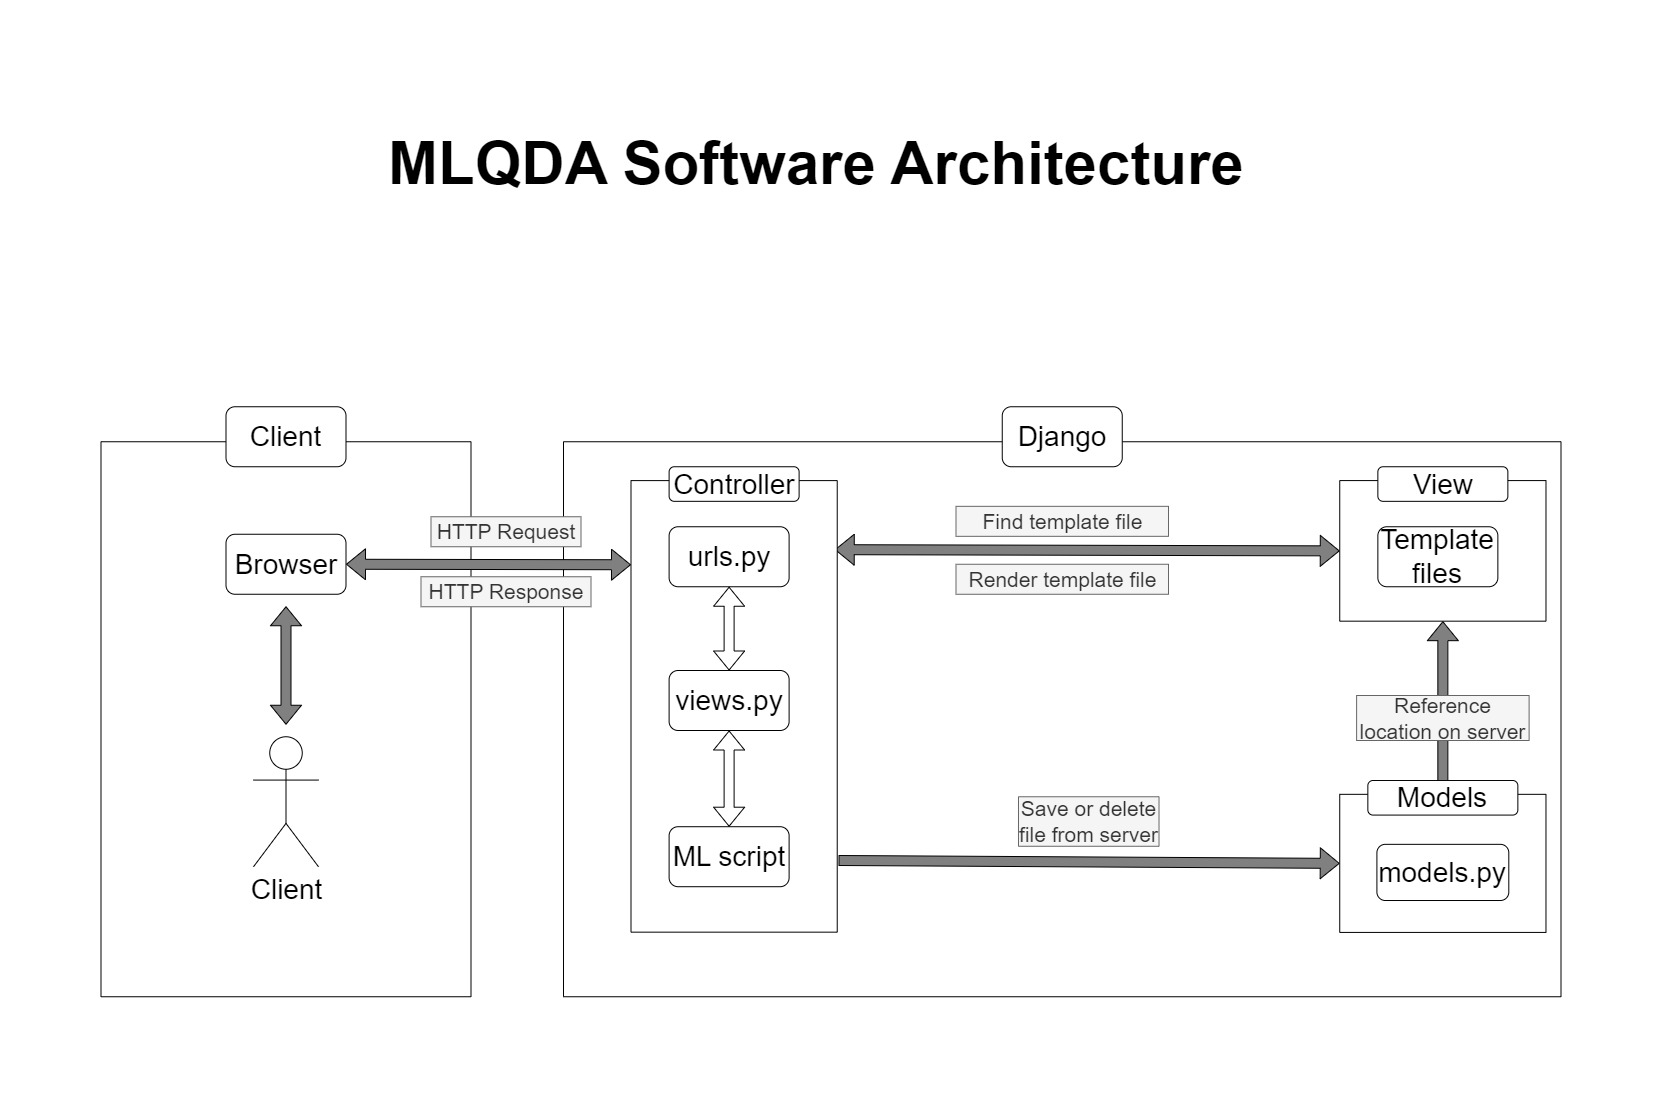
\includegraphics[width=1\linewidth]{images/mlqda_software_architecture_updated.jpg}    
    \caption{System Architecture diagram for the MLQDA project to represent the underlying logic of the final product.}
    \label{fig:mlqda-SA-diagram} 
\end{figure}

Users are represented in the \textit{Client} branch. A user interacts with the rendered interface of the system through a browser. The browser collects the user input and communicates them to the Controller section of the system. Data from the user is forwarded via HTTP Requests. On the other hand, the displayed information is presented to the user via HTTP Responses.

The \textit{Model} branch is focused on the data of the system. Its primary responsibilities include the storage, manipulation and retrieval of the data \citep{fowler2012patterns}. Within this system, these tasks are taken care of by the models.py file. They allow for the representation of the database system and all its features required by the site. Furthermore, this file directly links to the existing database management system. 

The \textit{View} section is responsible for the interface presented to the Client. This section queries the Model and compiles the results in a way that is presentable and understandable by the user \citep{fowler2012patterns}. The main sources for this are the HTML templates, which provide a user-friendly interface. However, some tasks concerning the interaction with the Model are delegated to the view.py file, as the HTML templates alone cannot interact with it.

The \textit{Controller} represents the underlying logic behind the system. Apart from handling communication with the Client, the Controller also acts as a channel between the View and the Model. Based on the user input, the Controller can modify the Model and update the View \citep{fowler2012patterns}. Within the Django Framework, the urls.py and the views.py files are responsible for providing this underlying logic for the system. They are in charge of the flow of the site and the handling of the user input. 

In addition to this architectural pattern, there is another extra layer within the Controller section. As part of the Controller branch, the \textit{ML Scripts} send and receive data from the views. In this regard, the views collect the data required for the \textit{ML Scripts} and invoke them. After the \textit{ML Scripts} perform their job, they return the results to the views to be displayed to the user. The \textit{ML Scripts} also access and delete file instances from the Model branch. 

\section{User Activity}
This section aims to explain a user session. This process showcases how a potential user might use the system. It also gives a more tangible situation where most features are used. While an activity diagram can be seen in Appendix \ref{appendix:b}, the rest of this section introduces the proposed workflow for new users.

\begin{itemize}
    \item New users access the home page
    \item The user reads the About and/or FAQ pages to get insight into how the system works
    \item The user navigates to the Analyser start page
    \item The user uploads the correctly formatted text files to the upload field
    \item After continuing, the user is presented with their results
    \item The user saves their results and leaves the page
    \item Upon leaving the page, all data connected to their session is deleted
    \item The user has trouble understanding the output, so they check the About and/or FAQ page again.
\end{itemize}

\section{Wireframing and Prototyping}

% Wireframes are the first step towards a tangible user-focused interface design. Their simplistic design allows developers to brainstorm and change elements without great effort. Most importantly, they present the system's layout and flow while giving a shared understanding and idea of it. Taking wireframes a step further, prototypes are more advanced wireframes that enable the integration of some of the logic of the system. While they take more effort than wireframes, they better highlight the possible interactions between the product and the user \citep{arnowitz2010effective}.
During this project's design phase, \textbf{Figma} was utilised to provide realistic wireframes that can be turned into interactive prototypes. By the end of the design process, a prototype was developed to represent the main features of the final product. This prototype ensured better communication with the customer and further settled the vision for the project's end goal. The prototype included a total of six wireframes covering all the must-have and should-have features. This section discusses two wireframes in depth. While the entire set of wireframes can be found in Appendix \ref{appendix:wireframes}, the interactive prototype is available on \href{https://www.figma.com/proto/XElvUvEeXKuAAlMz7AxEIu/ML_QUAL_ANALYSER?node-id=1-2&scaling=scale-down&page-id=0%3A1&starting-point-node-id=1%3A2}{figma.com} link.

The top of both Figure \ref{fig:mlqda-analyser-start-diagram} and Figure \ref{fig:mlqda-analyser-results-diagram} shows the navigation bar that outlines the main parts of the web app container. The central part of Figure \ref{fig:mlqda-analyser-start-diagram} focuses on the file upload feature of the product. As per the requirements, this page explains the expected formatting of the files and allows file upload. It also shows that results can be accessed with just one click after hitting \textit{Analyse}. 

Figure \ref{fig:mlqda-analyser-results-diagram} shows the result page, where users can find their corresponding results from their latest analysis on the site. The most important results are displayed on this page. Furthermore, this page allows users to download their results and an annotated version of their original files.  

\begin{figure}[H]
\centering
\begin{subfigure}{.5\textwidth}
    \centering
    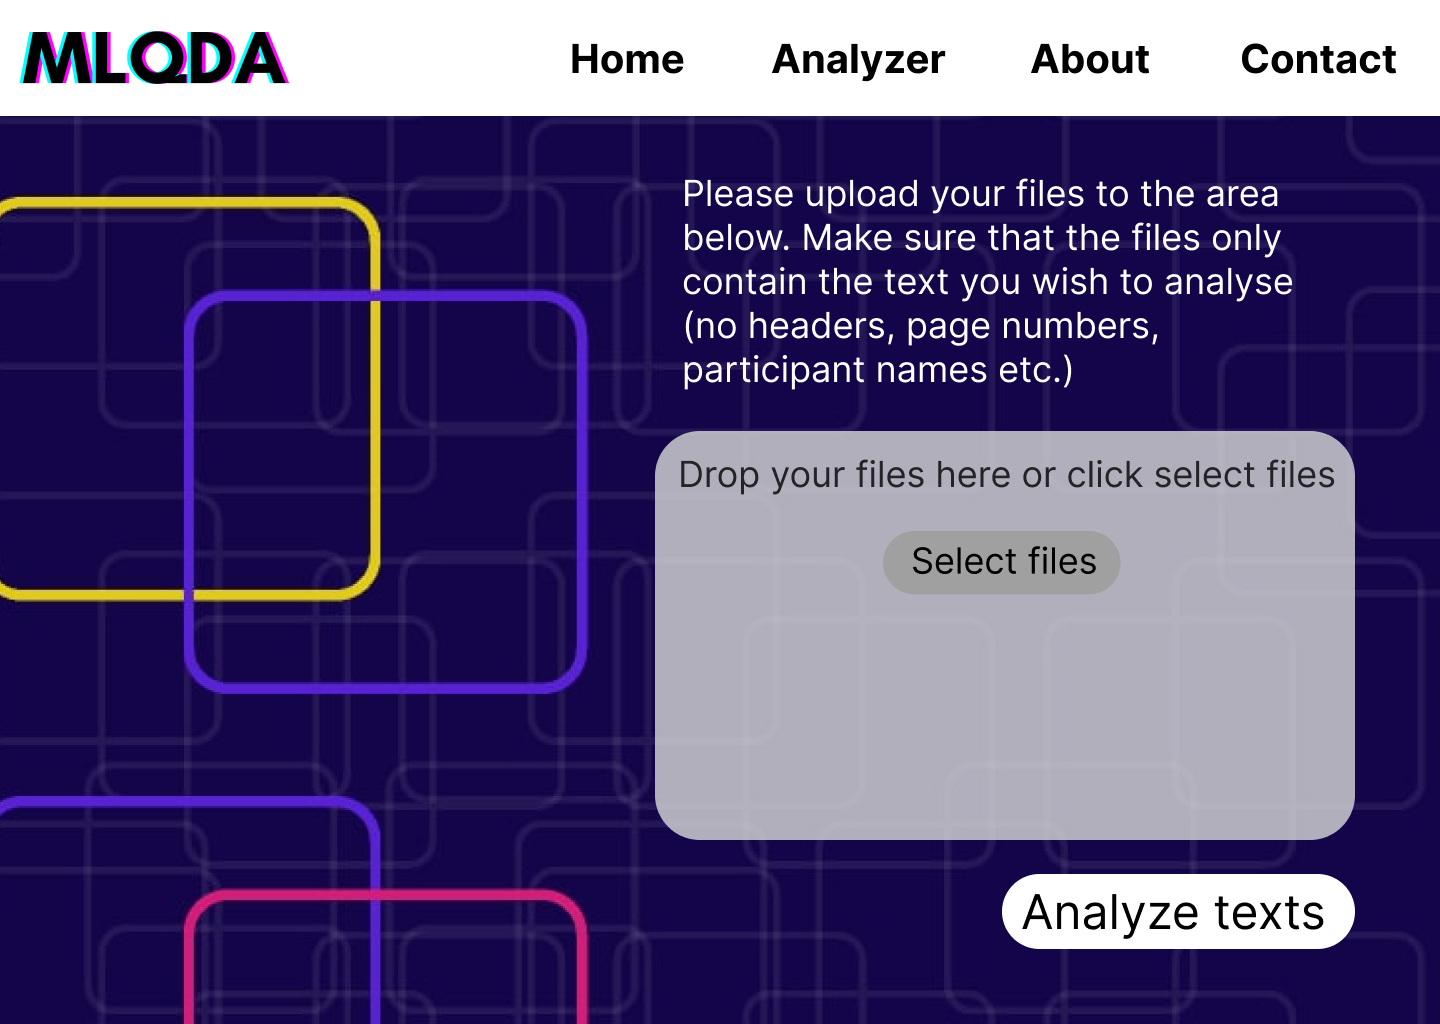
\includegraphics[width=0.95\linewidth]{images/Analyzer (start).png}
    \caption{Analyser starter page}
    \label{fig:mlqda-analyser-start-diagram} 
\end{subfigure}%
\begin{subfigure}{.5\textwidth}
    \centering
    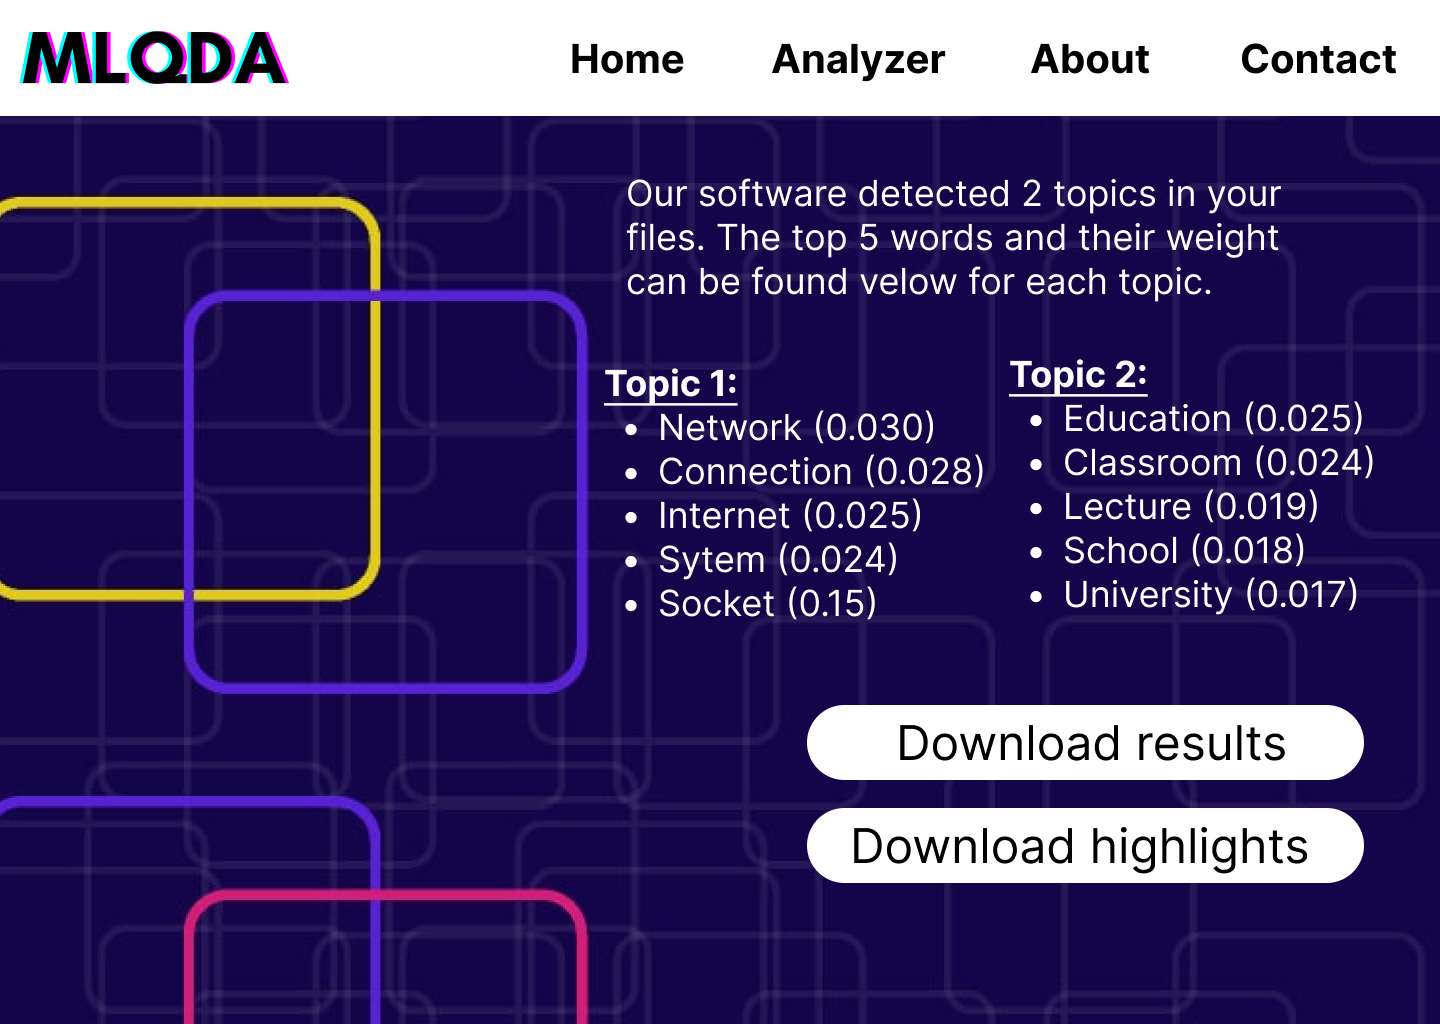
\includegraphics[width=0.95\linewidth]{images/Analyzer (results).png}
    \caption{Analyser starter page}
    \label{fig:mlqda-analyser-results-diagram} 
\end{subfigure}
\caption{Sample wireframes}
\label{fig:wireframes}
\end{figure}

\section{Database design}
The main section of the Model branch within the MVC architectural pattern deals with the representation of the data. One of the primary considerations for the system was processing and storing the data safely without any potential data breach. As the uploaded data can contain sensitive information, the product tries to keep files in the database for as little time as possible. Data keeps getting deleted after each analysis, so the system does not save the results. Adhering to this requirement resulted in a relatively simple database design, as seen in Figure \ref{fig:mlqda-ER-diagram}.

Under the current design, there are two entities, FileContainers and FileCollectors. The primary purpose of a FileContainer is to record a file's location. Apart from this, it also records a unique ID, a file name and a reference to a FileCollector. A FileCollector instance has a name and an ID. It is designed to record an analyser session and all related files.

Upon file upload, all files are saved as a FileContainer connected to the same collector. Throughout the analysis, more files could be created from these files, such as result files or highlights. These new files are also saved as their own separate FileContainer but still connected to the same FileCollector. 

\begin{figure}[H]
    \centering
    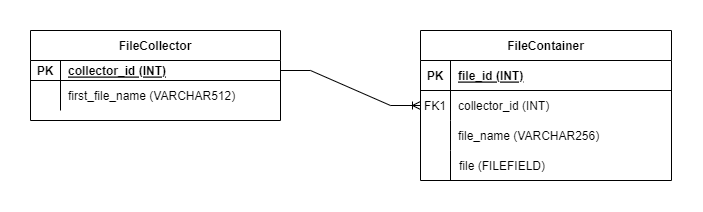
\includegraphics[width=1\linewidth]{images/mlqda_db.drawio.png}    
    \caption{ER diagram representing the structure of the underlying database structure}
    \label{fig:mlqda-ER-diagram} 
\end{figure}



\section{Choice of technologies}
% The previous sections of this chapter and the Requirements chapter outlined the technical requirements for this product. This next section introduces the chosen technologies to match these requirements and desires.

From the start of the project, the desired outcome was a lightweight web application. A web app allows wide accessibility while leaving space for security requirements. \textbf{Python 3} was identified as the primary programming language of the project stemming from the usage of machine learning techniques. Python has extensive libraries dealing with data science, natural language processing and machine learning. All of which are connected to the main requirements outlined before. To help with the processing of raw data input, \textbf{nltk}, \textbf{gensim} and \textbf{spacy} libraries were utilised. These libraries provided a cornerstone for the expected text analysis. The \textbf{Django Framework for Python} offered a flexible way to create lightweight web apps using the already established Python 3 language. Apart from its well-documented online presence, Django also provides all required user interactions already built in.

For the back-end database system, two things were considered. Besides being fast and responsive, the database needed to be well integrated with the previously chosen technologies, namely Django. As derived from the ER diagram on \ref{fig:mlqda-ER-diagram}, the database was not expected to handle complex tables. Furthermore, as the data is expected to be deleted, the database system was only expected to store data for a short time. An \textbf{SQLite} database was identified as a suitable technology for the above reasons.

Finally, different deployment options were also considered. Two potential choices were identified: PythonAnywhere and Railway. Both of these options offered an excellent level of compatibility with Django projects. Even though Railway offers integration with GitHub, in the end, \textbf{PythonAnywhere} was selected because of the better customisation opportunities and the familiarity with the product.

\section{Chapter Summary}
This chapter focused on the design process of the product before development started. It introduced the underlying System Architecture and showcased an intended session as an Activity Diagram. Furthermore, it also gave a walkthrough of the wireframes and the database design. Finally, the chapter covered the technologies used to develop the product.

The next chapter centres around the implementation of the product.
%==================================================================================================================================

\chapter{Implementation}
This chapter introduces the software engineering practices utilised during development, specifically focusing on the development method and the chosen version control system. Furthermore, this chapter covers the implementation of the system's key features and showcases the finished system.

\section{Software Engineering Practices}
\subsection{Development Method}
% For this project, several software development methodologies were considered. Both Agile and Scrum require a development team. However, the Waterfall methodology offers a framework for individual developers. Moreover, a comprehensive list of requirements was collected from an early stage in the project lifecycle, which is a prerequisite for the Waterfall methodology. As a result, Waterfall was the selected development method.

% Unfortunately, Waterfall is not without drawbacks as it assumes sequentially and linearity from the project, making it less flexible than most of its contenders. Some aspects of Agile were applied to make the development more flexible to overcome this issue.

% As per the waterfall methodology, the development started with the compilation of an extensive set of requirements that was followed by the design phase. Contrary to the waterfall methodology, the implementation, testing and deployment phases did not follow each other in sequential order. At this point, a more Agile-focused workflow was utilised to allow for creating smaller tasks and continuous testing and deployment.

%The collected list of requirements was considered as the order backlog for the project's lifecycle, so the overall progress was still essentially linear. Tasks were extracted from this list on a weekly basis. If these tasks included new features, unit testing was developed for them concurrently. Continuous testing allowed the development of a comprehensive testing suite at every point in the project.

%Once the project reached the stage of Minimum Viable Project and implemented all the must-have requirements, the product was deployed. From then on, the project was redeployed and updated when a sufficient amount of changes had occurred, usually monthly. Frequent deployment ensured that the product was viable outside the development environment and often highlighted server-side issues that were not present there. 

% Finally, the pilot evaluation began after reaching the desired outcome described by the requirements. From this moment onward, the project entered the maintenance phase as outlined by the Waterfall methodology. Updates and changes were made based on the input received from evaluators.

% To summarise, the software development structure followed the Waterfall method but utilised Agile techniques to allow smaller incremental changes and continuous testing and deployment. 

For this project, several software development methodologies were considered. Both \textbf{Agile} and \textbf{Scrum} require a development team, but the \textbf{Waterfall} methodology offers a framework for individual developers. Moreover, a comprehensive list of requirements was collected early in the project lifecycle, a prerequisite for the Waterfall methodology. As a result, \textbf{Waterfall} was the selected development method. Unfortunately, Waterfall is not without drawbacks as it assumes sequentially and linearity from the project, making it less flexible than most of its contenders. Some aspects of Agile were applied to make the development more flexible to overcome this issue.

As per the waterfall methodology, the development started with compiling an extensive set of requirements, followed by the design phase. Contrary to the waterfall methodology, the implementation, testing and deployment phases did not follow each other sequentially. At this point, a more \textbf{Agile}-focused workflow was utilised to allow for creating smaller tasks and continuous testing and deployment. Tasks were extracted from the list of requirements, and the corresponding tests were implemented simultaneously. After completing the must-have requirements, the project was deployed and frequently re-deployed to ensure viability outside the development environment. According to the Waterfall guidelines, the project entered the maintenance phase after the pilot evaluation.

To summarise, the software development structure followed the Waterfall method but utilised Agile techniques, which allowed smaller incremental changes and continuous testing and deployment.

\subsection{Version Control and Continuous Integration}
% Over the development process, Git was used as a version control system, while GitHub hosted a remote backup repository of the entire project. Git and GitHub were chosen due to familiarity and experience with these technologies. Furthermore, Git was easily integrated into Visual Studio Code, the primary development environment. This integration allowed for a more graphical representation of recent changes and a graphical way of calling commands related to Git.

% GitHub offers features to manage multiple branches within the same repository. Furthermore, it provides easy merging techniques in the form of Pull Requests. A version of Trunk Based development style was adopted to utilise these functionalities fully. This style involved the creation of three primary branches "main", "dev", and "deployment". The main branch contained the most recent fully functional version of the project. Running parallel to this was the Dev branch containing the latest development updates. Finally, the Deployment branch tracked the main branch as well. However, it included some specific settings to allow faster redeployment whenever required. Temporary branches were created based on the development branch and merged back via Pull Requests. Once enough changes were made to the development branch, a separate pull request was issued to the main and deployment branches, respectively.

% GitHub also allows Continuous Integration pipelines in the form of GitHub Actions. For this project, the pipeline included two main things: testing and linting. Every pipeline run started with building and testing the code base using unit testing. The results and coverage of these tests were presented on the console. The other focus was on linting using the flake package. This ensured that the quality of the code was sufficient. The pipeline was configured to run automatically whenever updates were pushed to the development and the main branches.

% The final feature offered by GitHub is issue tracking. As explained in the previous section, issues were created from the list of requirements on a weekly basis. These issues were sorted into larger, overarching Milestones for better organisation. New branches were usually created for these milestones, and they were merged upon completing all the issues in the corresponding milestone.

Over the development process, \textbf{Git} was used as a version control system, while \textbf{GitHub} hosted a remote backup repository of the entire project. \textbf{Git} and \textbf{GitHub} were chosen due to familiarity and experience with these technologies. Furthermore, Git was integrated into Visual Studio Code, the primary development environment. This integration allowed for a more graphical representation of recent changes and a graphical way of calling commands related to Git. A version of Trunk Based development style was adopted over the entire course of development. Furthermore, Continuous Integration and Issue Tracking were also part of the development process.

\section{Key Features}
%So far, this chapter has outlined the techniques utilised during implementation. Moving forward, t
This section will focus developed features of the system. Even though most of the container app consists of static pages to help and guide the user, there are a significant number of features throughout the dynamic section of the app. Considering the length constraints, three main features were chosen to showcase the code base at the end of development.

\subsection{File handling}
First and foremost, the site was required to handle the upload of various files. During the requirements gathering process, the most popular file extensions were identified to ensure that the site could be available for the largest audience. Users can upload their files on the starting pages for Topic Modelling or Sentiment Analysis, which display instructions and the most important information to guide the user. Furthermore, the expected file types are limited, so by default, the user cannot select files the system cannot handle. As machine learning scripts tend to be time-consuming, the user is provided with a JavaScript reminder not to leave or reload the site. 

After completing the upload, a series of utility functions read their content and convert them into the appropriate format. Considering PDF, DOCX and TXT file extensions, each file is assumed to be one separate document. On the other hand, the system assumes that each row is a separate document for CSV and XLSX files. Listing \ref{lst:read_docx} and \ref{lst:read_csv} showcases how individual DOCX and CSV files are handled, while Listing \ref{lst:read_all} presents the logic behind reading all the files and converting them into a list of documents, where all documents are strings.

The \textit{read\_docx} function reads in a file with .docx extension using the \textbf{docx} python library. The function iterates through the paragraphs of the document and collects them in a list. This list is then joined together and returned as a string. On the other hand, the \textit{read\_csv} function uses a slightly different logic to access the content of a file with a .csv extension. The entire file is read in as a \textbf{pandas} data frame. The content of the resulting data frame is then joined together by a unique string of characters to indicate the spacing between entries. Before returning the joined string, a helper function filters out all the characters that are not \textbf{latex} friendly. This is required because some result files are compiled using \textbf{latex}, so input characters must be cleaned.

The \textit{get\_datafiles} presented in Listing \ref{lst:read_all} deals with the internal logic of reading all the files. The function takes a list of paths as a parameter. While iterating through them, the corresponding reading function is called based on the file extension. For example, if a file has a .docx extension, the \textit{read\_docx} function is called. The obtained content of each file is appended to a list. Finally, the function returns this list where every element is the full content of a file.  

\begin{lstlisting}[language=python,
caption={Function to read in a single DOCX file.},
label=lst:read_docx]
def read_docx(file_path):
    document = docx.Document(file_path)
    document_text = []

    for paragraph in document.paragraphs:
        document_text.append(paragraph.text)

    text = ' '.join(document_text)
    return text
\end{lstlisting}
\newpage
\begin{lstlisting}[language=python,
caption={Function to read in a single CSV file.},
label=lst:read_csv]
def read_csv(file_path):
    my_csv = pd.read_csv(file_path, header=None)
    document_text = ' MLQDAdataBreak '.join(my_csv.iloc[:, 0])
    text = remove_nonlatex_chars(document_text)
    return text
\end{lstlisting}

\begin{lstlisting}[language=python,
caption={Function to read in all the files.},
label=lst:read_all]
def get_datafiles(path_list):
    full_text = []
    for file_path in path_list:
        if file_path.endswith(".txt"):
            text = read_txt(file_path)
        elif file_path.endswith(".pdf"):
            text = read_pdf(file_path)
        elif file_path.endswith(".docx"):
            text = read_docx(file_path)
        elif file_path.endswith(".csv"):
            text = read_csv(file_path)
        elif file_path.endswith(".xlsx"):
            text = read_xlsx(file_path)

        full_text.append(text)

    return full_text
\end{lstlisting}

\subsection{Topic Modelling process}

The first machine-learning script that MLQDA offers is Topic Modelling. This technique was identified as the higher-priority technique when gathering the requirements. There is considerable overlap and parallel between the theory and execution of Topic Modelling and Thematic Analysis. The code focusing on Topic Modelling was developed in an Object-Oriented style to provide a better and easier organisation of files and results. Based on a list of paths, the constructor for a topic modelling instance utilises the functions discussed in the previous section to access their content. The list of all the text is called a corpus. The first set of steps revolves around Natural Language Processing and deals with data cleaning. After the data is cleaned and transformed into an appropriate structure, the system concurrently runs multiple models and identifies the best of them. A more in-depth description of the workflow used in this class can be found in Appendix \ref{appendix:tm_workflow}.

Listing \ref{lst:mlqda_single_lda} highlights the \textit{run\_lda} function taking one parameter specifying the number of topics the model should look for. This is a container function within the \textbf{TopicModelling} class to utilise a \textbf{gensim} \textbf{LdaModel}. The required input \textbf{courpus} and \textbf{id2words} are already present within the instance. All hyper-parameters required for the \textbf{LdaModel} are arbitrarily set except for the number of topics, which is set based on the container function parameter. After the model has finished, the function appends it to a list collecting all the models for this instance. Finally, the individual model instance is returned to allow individual evaluation if necessary.

Listing \ref{lst:mlqda_dynamic_lda} shows the \textit{dynamic\_lda} function, which handles the concurrent aspect of the analysis. LDA requires looking for at least two topics, but there is no upper limit on the number of topics. However, to avoid overwhelming the system, the \textit{calculate\_topic\_threshold} function calculates the limit of maximum topics the system should look for. This is partially based on the number of input documents, but there is an upper limit of twelve to keep the system relatively fast. After calculating the maximum number of topics the system should look for, threads are created for each possible model. For example, if the maximum number of topics is five, the function creates four threads with models looking for two, three, four and five topics. Threads are created using the \textbf{threading} library, utilising the previously explained \textit{run\_lda} function. All the models are stored within the instance after starting and joining the threads. To identify the best version, a \textbf{gensim} \textbf{CoherenceModel} is constructed for each model. Based on the extracted coherence score, the highest-scoring model is retained in a separate field of the instance.

\begin{lstlisting}[language=python,
caption={Function to run a single LDA Topic Model},
label=lst:mlqda_single_lda]
    def run_lda(self, num):
        lda_model = gensim.models.ldamodel.LdaModel(corpus=self.structures['corpus'],
                                                    id2word=self.structures['id2word'],
                                                    num_topics=num,
                                                    random_state=100,
                                                    update_every=1,
                                                    chunksize=100,
                                                    passes=10,
                                                    alpha="auto")
        self.models.append(lda_model)
        return lda_model
\end{lstlisting}


\begin{lstlisting}[language=python,
caption={Function to concurrently run multiple LDA Topic Modelling.},
label=lst:mlqda_dynamic_lda]
    def dynamic_lda(self):
        topic_number = calculate_topic_number(len(self.datafiles))
        coherence_scores = []
        threads = []

        for i in range(2, topic_number):
            current_thread = threading.Thread(target=self.run_lda, args=(i, ))
            threads.append(current_thread)

        for t in threads:
            t.start()
        for t in threads:
            t.join()

        for current_model in self.models:
            current_coherence = CoherenceModel(model=current_model,
                                               texts=self.structures['trigram_texts'],
                                               coherence='u_mass')
            coherence_scores.append(current_coherence.get_coherence())

        max_coherence = max(coherence_scores)
        max_index = coherence_scores.index(max_coherence)
        max_model = self.models[max_index]

        self.lda_model = max_model
\end{lstlisting}



%===============================================================



\subsection{Sentiment Analysis process}
The second machine learning technique that the MLQDA site offers is Sentiment Analysis. Similarly to Topic Modelling, an Object-Oriented approach was taken to keep data organised, and an instance can be initiated primarily from the path to the files. Sentiment Analysis largely depends on its training set. The system uses the built-in VADER sentiment analyser from the \textbf{NLTK} python library. This implementation was trained on Twitter posts, so it gives the best results on similar types of data. However, breaking the document down into sentences brings it closer to those texts.

After using the utility functions previously introduced, the corpus is split into smaller parts. The content is divided into sentences for TXT, PDF, and DOCX files, while for CSV and XLSX files, each cell represents a unit. The reason for requiring smaller units of text originates from the training data set for the analyser. The analyser calculates a score for each of the entries. These are compound sentiment scores calculated from positive, negative and neutral sentiment scores. The scores range from -1 to +1, providing a two-way 100\% scale. The entry-based scores are also aggregated over every document and the overall corpus.

Listing \ref{lst:sa_csv_results} displays the \textit{create\_csv\_results} function, which is responsible for how a corpus is broken up, analysed individually then compiled into a CSV file. First,  the function iterates through the file contents connected to the current instance of \textbf{SentimentAnalyser} and splits the data based on the file extension. For each one of these split entries, a compound sentiment score is calculated using the \textbf{SentimentIntensityAnalyzer} from the \textbf{NLTK} library. Following this, a single line is compiled as a dictionary containing the file name, the whole entry and the corresponding sentiment score. When all the entries in all the files have been analysed, the function evokes the \textit{write\_csv\_file} helper function to write the results into a CSV file. Before returning the path to the result file, the function also creates a model to keep track of the file in the database.



\begin{lstlisting}[language=python,
caption={Function to compile results into a CSV file.},
label=lst:sa_csv_results]
    def create_csv_results(self):
        rows = []
        for file in self.datafiles:
            file_path = self.datafile_paths[self.datafiles.index(file)]
            file_name = os.path.basename(file_path)

            if file_name.endswith((".xlsx", '.csv')):
                sentences = file.split('MLQDAdataBreak')
            else:
                sentences = file.split(". ")

            for sentence in sentences:
                tag_removed_text = re.sub(r'@\w+', '', sentence)
                sentiment_analyser = SentimentIntensityAnalyzer()
                sentiment_scores = sentiment_analyser.polarity_scores(str(tag_removed_text))
                compound_score = sentiment_scores['compound']
                row = {"File Name": file_name,
                       "Entry": unidecode.unidecode(str(sentence)),
                       "Sentiment Score": compound_score}
                rows.append(row)

        path = write_csv_file(self.collector_id, rows)
        self.create_model(path)
        self.csv_result = path
        
\end{lstlisting}

\subsection{Compilation and storage of results}

After all the steps of Topic Modelling or Sentiment Analysis have been completed, the user is presented with the Results page as shown in Figures \ref{fig:tm_results_1}, \ref{fig:tm_results_2} and \ref{fig:sa_results}, respectively. An example for each type of analysis results can be found in the \textit{example\_results} folder within the compressed folder. At this point, the system deleted every reference to all the files and their contents to ensure security. The only related file is a zip file containing a variety of results. Users can access this by clicking download. Furthermore, they also have the option to delete this file from the server. Otherwise, the result file will stay on the server for up to an hour, and it will be deleted automatically afterwards.

Depending on the type of analysis, the system compiles a different set of results. These compilation functions are also part of the classes connected to the two types of analysers. The results for Sentiment Analysis consist of two files. First, a static PDF document containing an annotated version of the original input and guides on how to interpret them. The results are presented in a table, where one column lists all the entries while the other displays the corresponding sentiment score. The second file contains the same table but in a CSV format to allow more flexibility for the users to make manual changes.

On the other hand, Topic Modelling results include a few more files. Similarly to the Sentiment Analyser, the main results are presented in PDF files. Apart from including interpretation guides, this file also displays tables of an annotated and highlighted version of the original input. A new PDF file is created for every topic, and every document is presented in a separate table. The original input is broken down into smaller chunks. These chunks are highlighted if any of the high-importance topic terms are present in them. Furthermore, if a term is present, it is displayed next to the corresponding chunk. The same data is presented in a CSV file to allow greater flexibility and post hoc manipulation of the results. In addition, the top terms and their contribution is plotted and saved as a PNG file. This visualisation indicates the importance of each top term. Finally, two helper structures - id2word and corpus - are saved as a simple TXT file if the user wishes to analyse their cleaned data. 

Listing \ref{lst:mlqda_sa_result_compilation} demonstrates the \textit{compile\_results} function developed as part of the \textbf{SentimentAnalyser} class. First, the function creates a unique path based on the ID of the file collector model instance. All files connected to this \textbf{SentimentAnalyser} instance reference this ID number. A zip file is created with the \textbf{zipfile} package, and both result files are written to it. Then these files are manually removed from the server. Next, the function deletes the input files and removes all references to every file related to the analysis from the models and database. Finally, the function returns the path to the zip file.

\begin{lstlisting}[language=python,
caption={Function to compile results for Sentiment Analysis.},
label=lst:mlqda_sa_result_compilation]
    def compile_results(self):
        self.zip_name = str(str(self.collector_id)+str('_results.zip'))
        zip_path = os.path.join(settings.MEDIA_DIR, self.zip_name)
        with ZipFile(zip_path, 'w') as zip_results:
            zip_results.write(self.pdf_result, str(os.path.basename(str(self.pdf_result))))
            zip_results.write(self.csv_result, str(os.path.basename(str(self.csv_result))))
            os.remove(self.pdf_result)
            os.remove(self.csv_result)

        self.remove_input_files()
        self.create_model(zip_path)
        return self.zip_name
\end{lstlisting}

Listing \ref{lst:mlqda_delete_files} displays the \textit{delete\_all\_uploaded\_files} function responsible for deleting all unnecessary files from the server. There are two ways a file could stay on the server. Firstly, if there is an issue during analysis like faulty formatting or the user closes the page. Secondly, if the user fails to delete their results from the server manually. To ensure confidentiality with the users and overcome these potential issues, every file is deleted after an hour. This function is designed to detect and remove older files from the server.

The \textit{delete\_all\_uploaded\_files} function achieves that by gathering all the files in the database using Django's built-in model handlers. Then the function checks if the file was uploaded more than ten minutes ago or not. If it is an older file, both the file and the model are deleted from the system. Furthermore, this function also finds all the files in the upload destination directory and deletes all the files uploaded more than 10 minutes ago. These two loops cover all possibilities of how a file can stay on the server accidentally.

\textbf{PythonAnywhere} offers to run background commands recurringly. This feature was utilised to run the \textit{delete\_all\_uploaded\_files} function every hour. Listing \ref{lst:mlqda_automated_deletion} shows the shell commands to find and run the correct script. The first step is to enter the project's virtual environment, and then the command navigates to the required directory. Next, the Django shell environment is entered, from which the correct file is evoked. The commands result in running the function from Listing \ref{lst:mlqda_delete_files} and deleting all unrequired files.

\begin{lstlisting}[language=python,
caption={Function to find and delete all files from analysis.},
label=lst:mlqda_delete_files]
def delete_all_uploaded_files():
    collectors = FileCollector.objects.all()
    print("deleted files:")

    for collector in collectors:
        files = FileContainer.objects.filter(first_name=collector)

        for file in files:
            if os.path.exists(str(file.file)):
                creation = os.path.getmtime(str(file.file))
                current = time.time()
                age = (current - creation)/60
                if age > 10:
                    print(str(file.file))
                    os.remove(str(file.file))
                    file.delete()
                    collector.delete()

    filepath = os.path.relpath(settings.MEDIA_DIR, start=os.curdir)
    for file in sorted(os.listdir(filepath)):
        file_path = os.path.join(filepath, file)
        creation = os.path.getmtime(file_path)
        current = time.time()
        age = (current - creation)/60
        if age > 20 and os.path.exists(file_path):
            print(str(file_path))
            os.remove(file_path)
\end{lstlisting}
\newpage
\begin{lstlisting}[language=bash,
caption={Shell script to execute file deletion.},
label=lst:mlqda_automated_deletion]
workon mlqdaenv && cd ~/mlqda/src/mlqda_project && python manage.py shell < "mlqda/file_cleanup.py"	

\end{lstlisting}

\section{Finished System}
Figure \ref{fig:mlqda_tm_start_example} shows the interface of the system during Topic Modelling. A comprehensive representation of the user interface can be found in \ref{appendix:gui}.

\begin{figure}[H]
\centering
    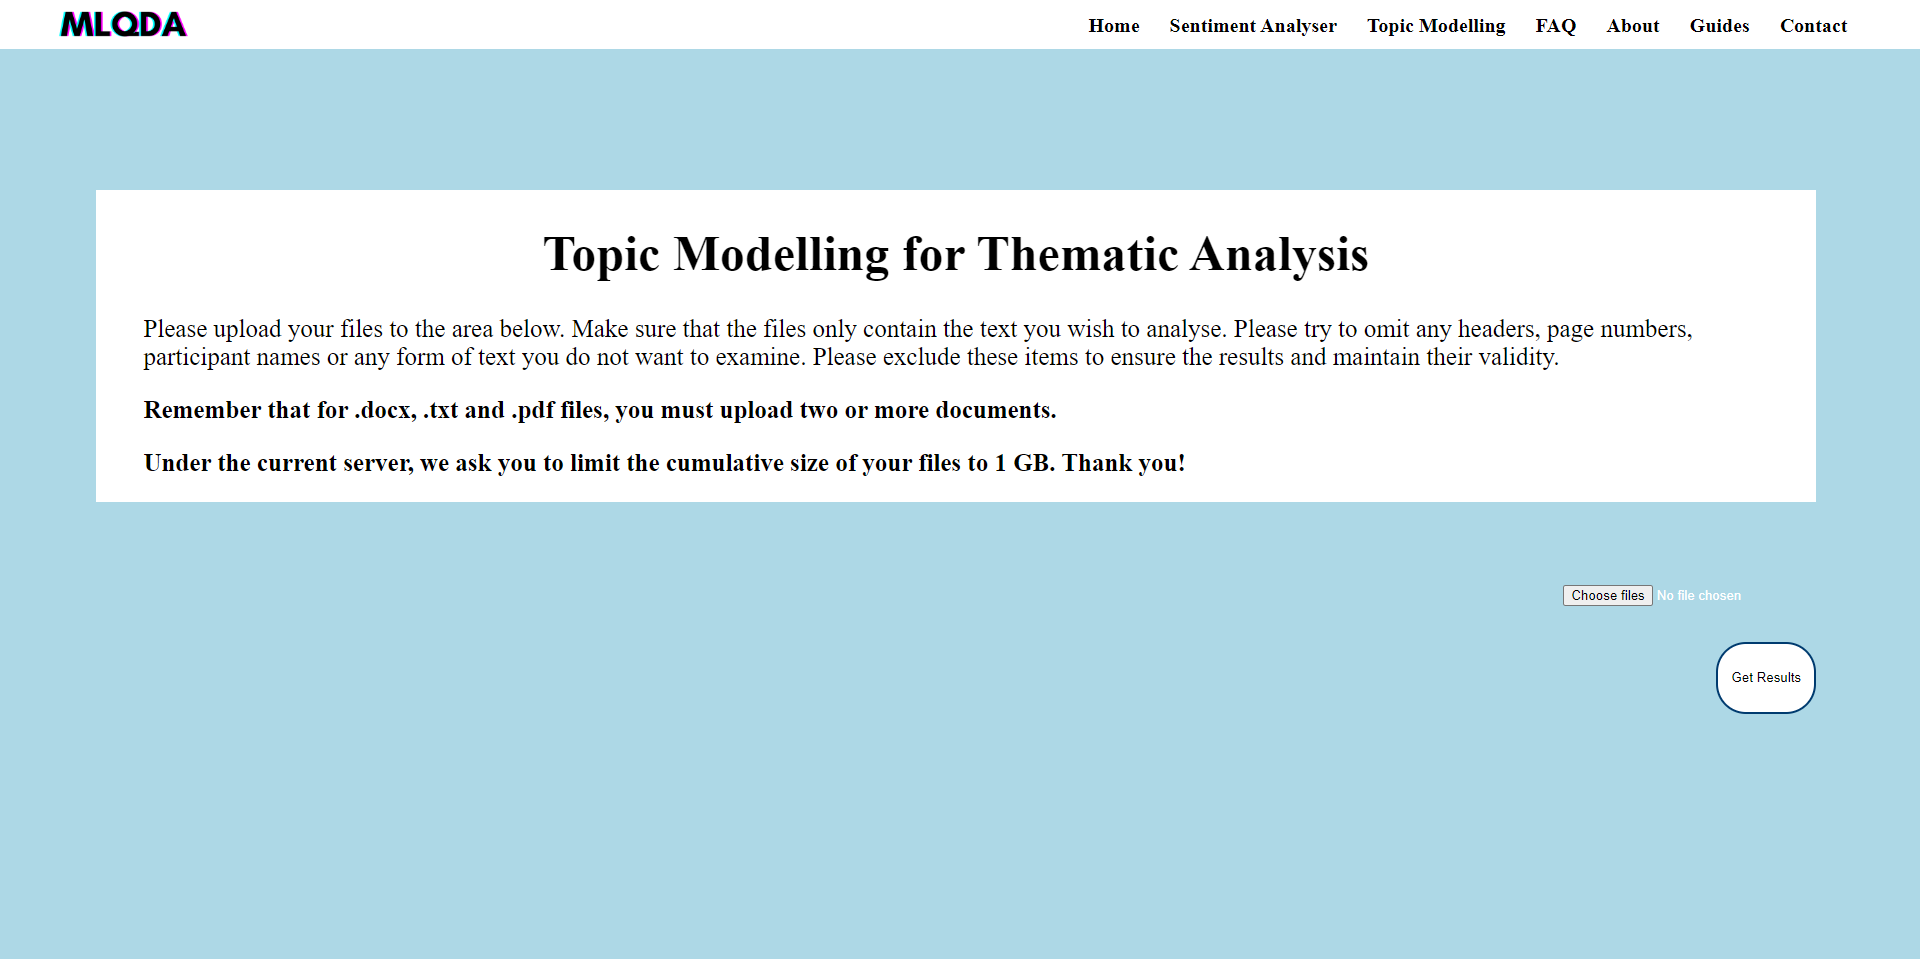
\includegraphics[width=0.95\linewidth]{images/tm_start.png}
    \caption{Start page for Topic Modelling}
    \label{fig:mlqda_tm_start_example} 
\end{figure}

Within the compressed folder for this project, there is a \textit{presentation/UserGuide.pdf} that provides a step-by-step guide to using the system and accessing the results. Furthermore, example results based on the test data are available in the same folder. Moreover, a presentation video called \textit{presentation/2472886t.mp4} includes a walk-through of the final version of the system, which is also available online \href{https://gla-my.sharepoint.com/:v:/g/personal/2472886t_student_gla_ac_uk/ERPu8Y0Ln7pMtQkLxoOH7mQBA9LOqRGrGdXHpU5_Cwm9ng?e=fjSEA3}{by clicking here}. Finally, a series of \textit{ReadMe.md} files describe the contents of the compressed folder.

The version achieved at the project's end is deployed, and it can be accessed through the following link: \href{https://zsolttakacs2000.pythonanywhere.com/mlqda/}{https://zsolttakacs2000.pythonanywhere.com/mlqda/}. Alternatively, the same version can be locally launched using the guidance from \textit{src/readme.md} from the compressed folder or from the following repository: \href{https://github.com/zsolttakacs2000/mlqda/tree/main}{https://github.com/zsolttakacs2000/mlqda/tree/main}.

\section{Chapter Summary}
This chapter focused on the details of implementing the MLQDA system. First, the chapter outlined the development method, a mixture of Waterfall and Agile methodologies. Then the chapter described the Version Control System and its usage. Secondly, the chapter also focused on the implemented key features like file handling, topic modelling, sentiment analysis and result compilation. Finally, the chapter introduced a series of references and guides for the finished system.

The next chapter revolves around two main aspects: Testing and Evaluation.

%==================================================================================================================================

\chapter{Testing and Evaluation}
This chapter details how the MLQDA system was tested and evaluated. First, the unit test suite is introduced, followed by the description of manual testing. Secondly, the user evaluation is explained, focusing on both the pilot and the final user evaluation. 

\section{Testing}
Testing is an integral part of software development. There are several types of testing techniques depending on the project. Over the development of the MLQDA site, the two main categories of testing utilised were unit testing and manual testing. The main goal of developing a testing suite was to confirm the development and logic behind all features derived from the requirements.

\subsection{Test Data}
The contents of a series of BBC articles were extracted for both manual and unit testing. The full texts are available in the compressed folder under the \textit{testing\_files} folder. Using these texts not only allowed to test features but ensured consistency and accuracy across trials
\subsection{Unit Testing}
Unit testing allowed the in-depth inspection of smaller pieces of the software. The built-in testing library was utilised from Django to develop the unit tests. Apart from being well-documented, this library also allowed the easy testing of Django-specific features.

The testing suite was continuously updated throughout the project to accommodate the newest features. By the end of development, a total of 34 unit test cases were created. These were categorised into four smaller subleases representing different aspects of the system. \textit{ViewTests} focused on the logic of the web app container and the Django implementation. \textit{TopicModellingTests} and \textit{SentimentAnalysisTests} were focused on the two machine-learning script and their results. They used preexisting test files to confirm that obtained results were as expected. Finally, \textit{UtilsTests} included test cases about utility and helper functions. These functions revolved around handling files, like reading and compilation.

As testing was part of the Continuous Integration pipeline, versions that did not pass all the tests were rejected from merging back to the development branch. As seen in \ref{fig:mlqda-coverage}, by the end of the development, the unit tests covered 1059 statements out of 1100, resulting in a 96\% coverage within the code base. Many of the missing statements originate from the utility function responsible for deleting old files. This feature could not be tested without pausing the testing suite for ten minutes.

\begin{figure} [H]
    \centering
    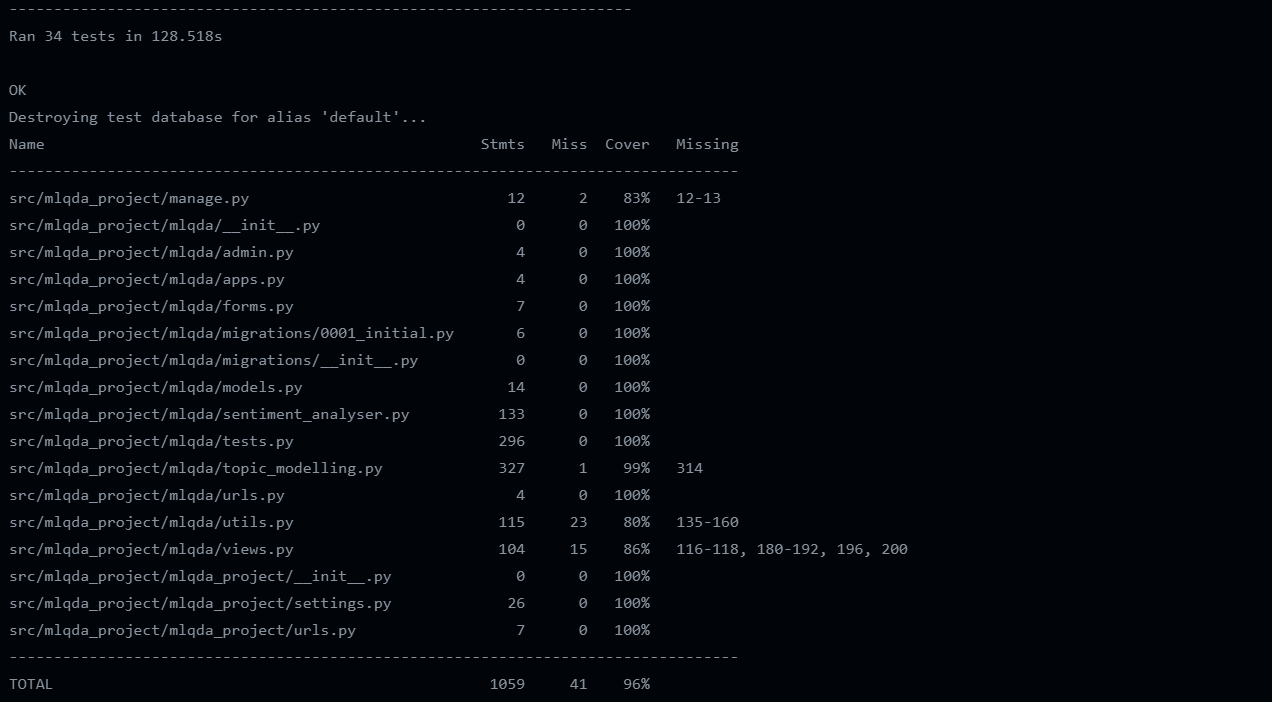
\includegraphics[width=1\linewidth]{images/mlqda_coverage.png}
    \caption{Unit test coverage of the MLQDA system}
    \label{fig:mlqda-coverage} 
\end{figure}


\subsection{Manual Testing}
While unit testing is perfect for checking the underlying logic, there are some aspects it cannot cover. These untested characteristics of the system were mainly related to the front-end design and the non-functional requirements. During manual testing, the deployed version of the system was thoroughly checked on two different machines. The main focus lay on the system's availability, performance and usability. Availability was tested by checking the design on multiple screen sizes and different machines. Performance and usability were tested by manually performing tasks on the existing test files. This testing procedure allowed the confirmation of the responsiveness and intuitive user experience.

A table was created based on the requirements lists to ensure consistency and rigour for manual testing. Figure \ref{fig:manual_testing} displays the manual testing table at the final testing. This table allowed tracking all aspects of the system that was tested regularly. This manual testing procedure has occurred at least after every redeployment, but most often, it was executed after every commit. Five of the eight manual user test scenarios focused on functional requirements, while three covered non-functional ones. 
\begin{figure}
    \centering
    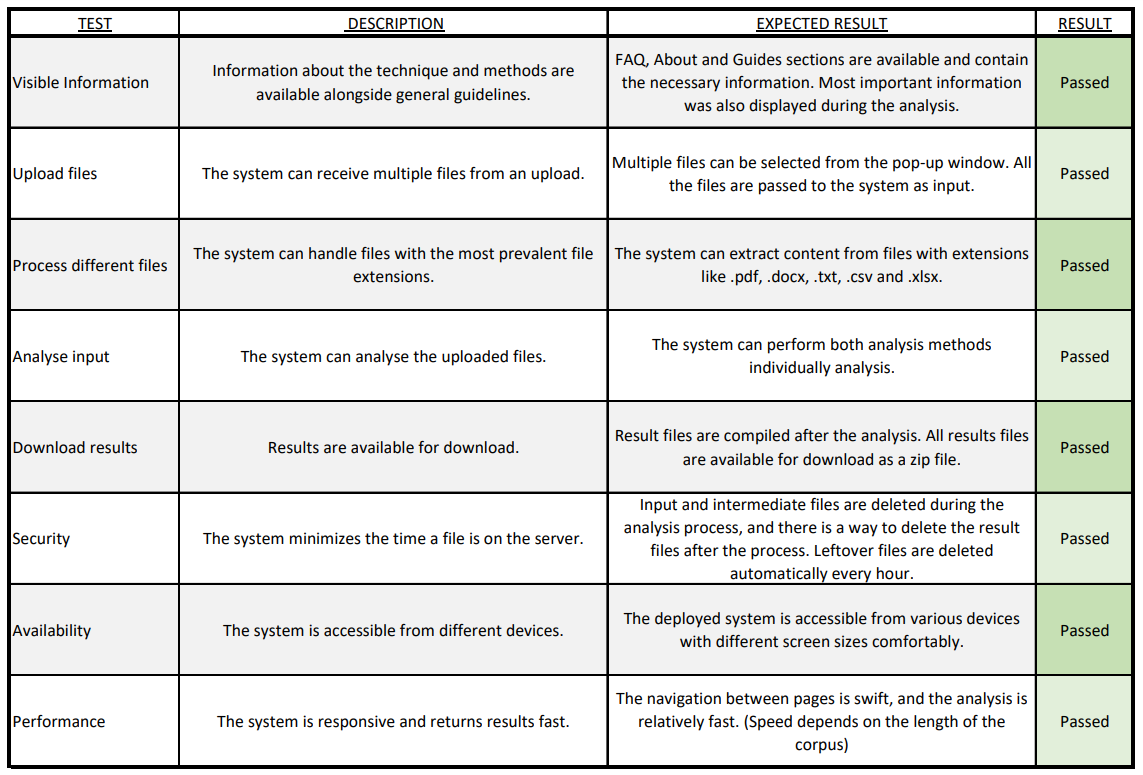
\includegraphics[width=1\linewidth]{images/manual_testing_table.png}
    \caption{Manual testing table at the end of development}
    \label{fig:manual_testing} 
\end{figure}


\section{Pilot User Evaluations}
Thus far, this chapter has focused on testing the finished system. However, a user's perspective is vital to record to evaluate a system entirely. For this reason, two types of user evaluations were conducted for this project. The first was an unstructured pilot evaluation to get general feedback about the system, followed by a more structured final user evaluation. 

The first type of evaluation of the product involved an unstructured review of the system. A lecturer with many years of qualitative data analysis experience was recruited through the project supervisor's help to try out the application and provide general feedback. Asking an expert to use the software in a real-life scenario gave insight into the possible missing features and whether the application can perform as expected.

After the first round of piloting, it was clear that while the idea was welcomed, the execution could have been better at the time. It was evident that the types of acceptable files needed to be extended. Previously only .pdf, .docx and .txt files were excepted. However, this evaluation resulted in the additional implementation of functionalities allowing users to work with .csv and .xlsx files. They also noted the need for a guide that provides a more user-focused walkthrough of the application rather than explaining the technical details. After fixing these shortcomings, the same evaluator was asked to provide more feedback considering that the system could work with more file extensions.

The second iteration of the pilot evaluation gathered more thorough feedback. Most importantly, the feedback praised the simplicity and easy usage of the application compared to NVivo. However, a few more suggestions were made on how to improve the application. Firstly, more organisational tips were shared regarding the provided help on the system. More importantly, the static nature of the results was identified as a possible negative aspect. Until that point, the main result document was a PDF file containing a table and description of the results. However, it was highlighted that better ways of presenting the results might exist. Their suggestion indicated the wish for the results to come in an editable .csv format to refine the obtained results manually. After this suggestion, functionalities were developed to return an additional .csv formatted result file for topic modelling and sentiment analysis.

\section{Final User Evaluation}
Implementing the issues identified in the pilot user evaluations ensured the system was ready for large-scale evaluation. The final user evaluation aims to measure the usability of the system as a whole from various perspectives.

\subsection{Methodology}
Implementing the issues identified in the pilot user evaluations ensured the system was ready for large-scale evaluation. The final user evaluation aims to measure the usability of the system as a whole from various perspectives.

\subsubsection{User Tasks: } Four user tasks were created to cover the most important functionalities of the system. The first two asked participants to navigate to certain parts of the web app to learn more about the underlying processes and requirements. The second two tasks asked them to perform two analyses, sentiment analysis and topic modelling. Example files from the testing data provided a common starting point. Participants had to indicate whether they completed each one of the tasks.

\subsubsection{System Specific Questions: } This section of the questionnaire was followed by eight system-specific questions where participants indicated how much they agreed with the statements on a five-point Likert scale. The first four focused on whether people found the provided guides helpful. Questions five to seven focused on the understandability of results. The final question revolved around a proposed feature, which was mentioned in the pilot evaluations regarding the manual modification of results. The system-specific questions were as follows:
\begin{enumerate}
    \item While completing the tasks, I referred to the FAQ, Guide and/or About sections.
    \item While completing the tasks, I found the information on the FAQ page useful.
    \item While completing the tasks, I found the information on the About page useful.
    \item While completing the tasks, I found the information on the Guide page useful.
    \item I found the Sentiment Analysis results clear and useful.
    \item I found the Thematic Analysis results based on Topic Modelling clear and useful.
    \item I found that the site offers an adequate amount of information for users about the applied machine-learning techniques.
    \item I would find updating the results manually an excellent addition to the system.
\end{enumerate}

\subsubsection{System Usability Scale: } The fourth part of the survey uses the System Usability Scale (SUS) by \cite{brooke1996sus}. It is a standard and well-used scale in the industry to measure the usability of a system that has continuously had good levels of reliability and validity \citep{lewis2018system}. It consists of ten statements, which the participants have to rate on a Likert scale of one to five. Appendix \ref{appendix:user_eval} contains a comprehensive list of all the SUS questions.

\subsubsection{Comments and Suggestions: } The final section allowed participants to leave comments and suggestions regarding the entire system. These questions were utilised to capture any issues or suggestions the previously described ones failed to cover.

\subsection{Results}
Throughout the evaluation period, thirteen participants filled out the online survey. The script used to analyse the collected data can be found in the \textit{data} folder within the compressed folder, alongside the original data set. Furthermore, several visualisations can be found in Appendix \ref{appendix:eval_results}. Table \ref{table:mlqda_demographic_table} presents the responses to the demographic questions. This suggests a wide range of expertise in the utilised techniques among the participants. As Figure \ref{fig:system_specific_visuals} shows, most evaluators found the provided guides useful. Furthermore, most of them also found the different types of results clear and useful. Many of them also supported the addition of manual result alteration as outlined in the pilot user evaluation.

Table \ref{table:mlqda_sus_table} displays the obtained SUS scores for each evaluator. This score is calculated through a series of steps, including getting the value for each response, summing all the values and multiplying that by 2.5. Using this process outlined by \cite{brooke1996sus}, the average SUS score was \textit{82.31}. Figure \ref{fig:sus_visualisation} displays the spread of final scores amongst the evaluators.

\begin{table}[H]
    \centering
    \begin{tabular}{|l|>{\centering}m{0.12\textwidth}|c|c|c|>{\centering\arraybackslash}m{0.1\textwidth}|}
    \hline
        \textbf{I am familiar with...} & \textbf{Strongly Disagree} & \textbf{Disagree} & \textbf{Neutral} & \textbf{Agree} & \textbf{Strongly Agree} \\ \hline \hline
        \textbf{Qualitative Data Analysis} & 1 & 2 & 3 & 6 & 1 \\ \hline
        \textbf{Sentiment Analysis} & 3 & 6 & 2 & 2 & 0 \\ \hline
        \textbf{Thematic Analysis} & 2 & 4 & 3 & 2 & 2 \\ \hline
        \textbf{Topic Modelling} & 2 & 4 & 4 & 3 & 0 \\ \hline
    \end{tabular}
    \caption{Counts for each demographic question}
    \label{table:mlqda_demographic_table}
\end{table}


\begin{table}[H]
    \centering
    \begin{tabular}{|>{\centering}m{0.12\textwidth}|c|c|c|c|c|c|c|c|c|c|>{\centering}m{0.06\textwidth}|>{\centering\arraybackslash}m{0.06\textwidth}|}
    \hline
        \textbf{Participant} & \textbf{Q1} & \textbf{Q2} & \textbf{Q3} & \textbf{Q4} & \textbf{Q5} & \textbf{Q6} & \textbf{Q7} & \textbf{Q8} & \textbf{Q9} & \textbf{Q10} & \textbf{Total} & \textbf{SUS score} \\ \hline\hline
        \textbf{1} & 3 & 4 & 4 & 4 & 3 & 4 & 4 & 4 & 4 & 3 & 37 & 92.5  \\ \hline
        \textbf{2} & 3 & 4 & 4 & 4 & 2 & 3 & 4 & 4 & 3 & 4 & 36 & 90  \\ \hline
        \textbf{3} & 1 & 1 & 1 & 3 & 2 & 2 & 1 & 2 & 2 & 3 & 18 & 45  \\ \hline
        \textbf{4} & 4 & 3 & 4 & 4 & 3 & 4 & 3 & 4 & 3 & 3 & 36 & 90  \\ \hline
        \textbf{5} & 4 & 2 & 2 & 3 & 3 & 3 & 1 & 3 & 2 & 4 & 28 & 70  \\ \hline
        \textbf{6} & 3 & 3 & 4 & 4 & 3 & 4 & 4 & 3 & 2 & 4 & 35 & 87.5  \\ \hline
        \textbf{7} & 3 & 3 & 4 & 2 & 4 & 4 & 4 & 4 & 3 & 3 & 35 & 87.5  \\ \hline
        \textbf{8} & 3 & 3 & 3 & 4 & 2 & 2 & 4 & 1 & 3 & 3 & 26 & 65  \\ \hline
        \textbf{9} & 4 & 4 & 4 & 4 & 4 & 4 & 0 & 4 & 4 & 4 & 36 & 90  \\ \hline
        \textbf{10} & 2 & 4 & 4 & 4 & 4 & 0 & 4 & 4 & 4 & 2 & 32 & 80  \\ \hline
        \textbf{11} & 4 & 4 & 4 & 4 & 4 & 4 & 4 & 4 & 4 & 1 & 37 & 92.5  \\ \hline
        \textbf{12} & 4 & 4 & 4 & 3 & 4 & 4 & 4 & 4 & 4 & 4 & 39 & 97.5  \\ \hline
        \textbf{13} & 2 & 4 & 3 & 3 & 4 & 4 & 3 & 4 & 3 & 2 & 33 & 82.5  \\ \hline
    \end{tabular}
    \caption{SUS scores from all evaluators}
    \label{table:mlqda_sus_table}
\end{table}

\begin{figure}[H]
    \centering
    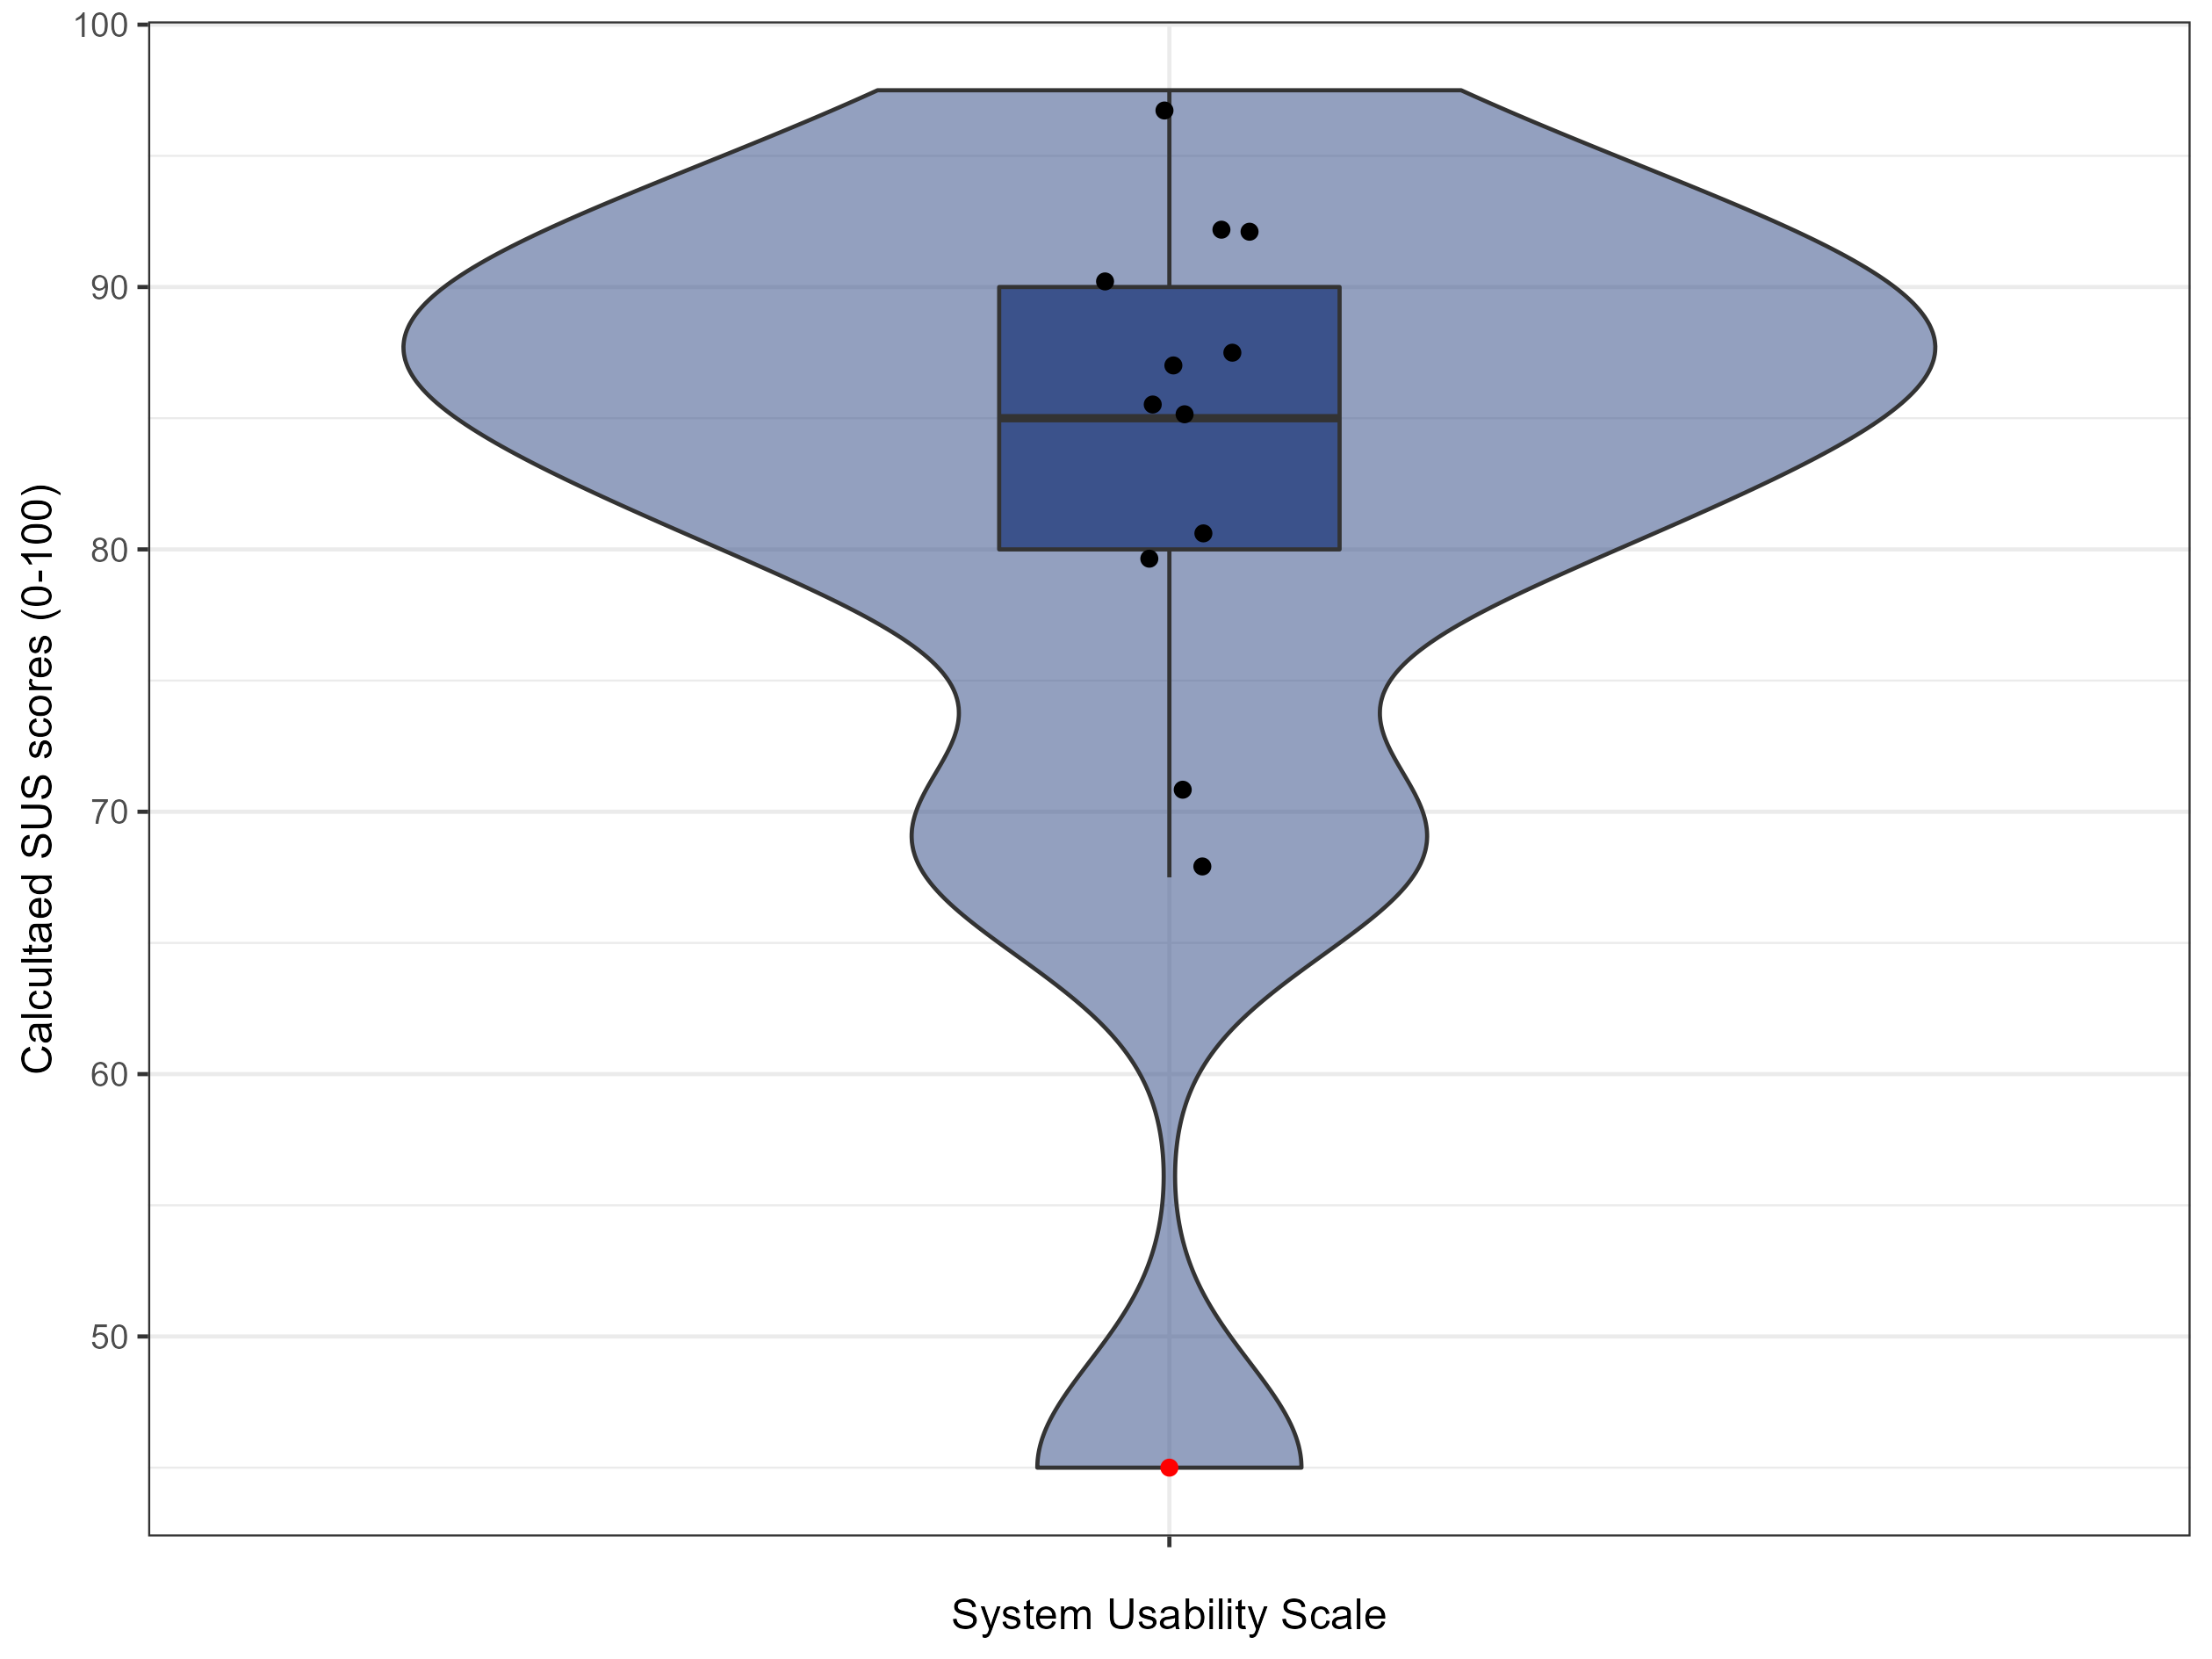
\includegraphics[width=0.65\linewidth]{images/sus_violin.png}
    \caption{Visualisation of SUS scores}
    \label{fig:sus_visualisation} 
\end{figure}


\subsection{Discussion of Results}
\cite{bangor2008empirical} stated that a SUS score of 70 has been used as a \textit{"rule of thumb"} to identify usable systems. According to this convention, the mean SUS score for the MLQDA system (\textit{M=82.31}) indicates a very usable product. However, it is important to note that two of the individual scores were under this threshold. Nonetheless, the general consensus among the evaluators favoured the system. 

Apart from quantitative data, the questionnaire also collected more qualitative responses via open-ended questions. Appendix \ref{appendix:user_eval_qual} presents the full list of answers. Regarding the general feedback about the entire system, many evaluators highlighted the user-friendly nature of the site labelling it \textit{"Very approachable and easy to use."}. On the other hand, multiple participants had issues with the presented information about how the system works. In these cases, the users lacked targeted instructions on how to use the system or interpret the results. While these instructions exist on the site, one for the evaluators called for the reorganisation of these to avoid \textit{"having to go the FAQ [page]"}. 

These comments were further iterated when asked about potential additions to the system. Most of these responses suggested a more comprehensive integration of guides within the system's main parts to provide a better workflow for first-time users. Apart from a slight design suggestion, one of the respondents suggested the option to download the result files individually instead of a compressed folder containing all the different files.

\subsection{Limitations}
One of the biggest limitations of this evaluation was the objectively small sample size. While almost all responses suggested that the evaluators were happy with the tested product, the small sample size prevented the conclusion of generalised ideas. The evaluation process would benefit from a larger cohort of evaluators to obtain a clearer picture of a future system's usability.

The existing solutions were a big part of the requirement-gathering process. So the evaluation would have also benefited from comparing this system to some of the existing applications. However, this would significantly increase the required resources for evaluation, so this might be more appropriate closer to the final stage.  

While there were a few identified limitations, the general consensus drawn from them is that system is pleasant to use. These results suggest the product's viability at this point in development and in this scope. Furthermore, they support the initiative to continue developing it.

\section{Chapter Summary}
This chapter focused on how the MLQDA system was tested and evaluated. Unit testing and manual testing covered any logical issues regarding the application, while user evaluation indicated the system's usability from a user perspective. The next chapter will summarise the entire work while offering insight into possible future work and reflection on the project.


%==================================================================================================================================

\chapter{Conclusion}

This chapter aims to summarise the dissertation and give an overall view of how the MLQDA system was developed and evaluated. Furthermore, this chapter will introduce ideas for future work and briefly reflect on the entire body of work.

\section{Summary of work}
As suggested by various academic sources, integrating machine learning techniques into qualitative data analysis methods could improve generalisability, validity and reproducibility. While some of the existing software supporting qualitative researchers move more and more towards these solutions, they all offer a highly complex environment for an expensive license. The MLQDA system was designed and developed to cover all these issues. The final software presents a free system that allows the easy analysis of textual qualitative data.

Requirements were gathered based on evaluating existing applications and intensive research into the theoretical background. These requirements were then prioritised with the \textit{MoSCow} technique. A \textbf{python}-based \textbf{Django} web application was designed and then developed based on these requirements. Throughout the development life cycle, all identified requirements have been implemented. 

The evaluation of the system was achieved in two aspects: testing and user evaluation. A comprehensive unit test suite was developed alongside the implementation of the product, which covered a significant portion of the code base. Furthermore, user evaluation took place in multiple steps. A third-party expert conducted two rounds of pilot evaluation, which helped identify some shortcomings of the first version of the system. After integrating their feedback, a more extensive system evaluation took place. Both its quantitative and qualitative sections revealed that the evaluators enjoyed using the system. However, they also suggested the better utilisation of guidance during the workflow to help first-time users.

\section{Future work}
While most requirements were developed, some features detailed on the \textit{Would be nice to have} remain unimplemented. Most notably, this includes an executable desktop version of the system. A version like this would allow more security for the users as the files would strictly stay on the user's machine rather than uploading to an external server. While this project's scope required one type of machine learning and another was categorised as low priority, the product might benefit from additional machine learning techniques. For example, with a sufficient training set from the user, the product could automate data labelling and coding using text classification methods. Furthermore, scaling up the processing power behind the system could allow more dynamic Topic Models. Currently, only the number of topics is not pre-set but chosen based on the best result, but the rest of them are left on base settings. However, with more resources, other parameters could be refined and investigated for better results.

During development, the \textbf{pyLDAvis} library was used to create more precise and interactive visualisations of the LDA Topic Modelling output. However, as the library was dependent on libraries with close deprecation warnings, it was taken out of the finished system. Because these visualisations are extremely extensive, it would be worth looking into manually developing the library so that it would not depend on deprecated libraries anymore.

As the responses from the pilot user evaluation suggested, there is a need for a feature that allows the manual altering of the results. While the main suggestions were implemented by providing a CSV version of the result table, this could be further developed. For example, allowing users to manually refine the identified topic words could be supported by the highlighting feature to represent the results confirmed by the user. This could be achieved by an additional step or by creating a more dynamic document format.

Even though intensive care was put in to support researchers unfamiliar with machine learning techniques, some feedback indicated the need for more thorough help during the automated analysis and how to interpret the results. Moreover, the evaluation responses suggested a whole new feature of individual file download. This feature would allow users to select which files containing the results they are interested in and download them individually rather than as part of a compressed folder. 

\section{Reflection}
The most frequent issues throughout the project arose from time management. Finding an appropriate balance between depth and effort for this individual project for joint honours was often an issue. However, the time management skills learnt previously from the course and the supervisor's feedback helped keep the project on track. Even though most of the technologies were familiar, the project still required a focused and in-depth knowledge of each. As individual work was frequently promoted throughout the course, getting more expertise with these technologies was quickly overcome. Finally, the final user evaluation would have benefited from a slightly larger sample, so in future work, there has to be a more efficient way to collect responses. Ultimately, the developed system achieved what it set out to achieve. Hopefully, in the future, it can be further developed and improved into a more well-rounded application. 
%==================================================================================================================================
%  APPENDICES  

\begin{appendices}
\chapter{Ethics Checklist}
\label{appendix:ethics}

\begin{figure}[H]
\centering
    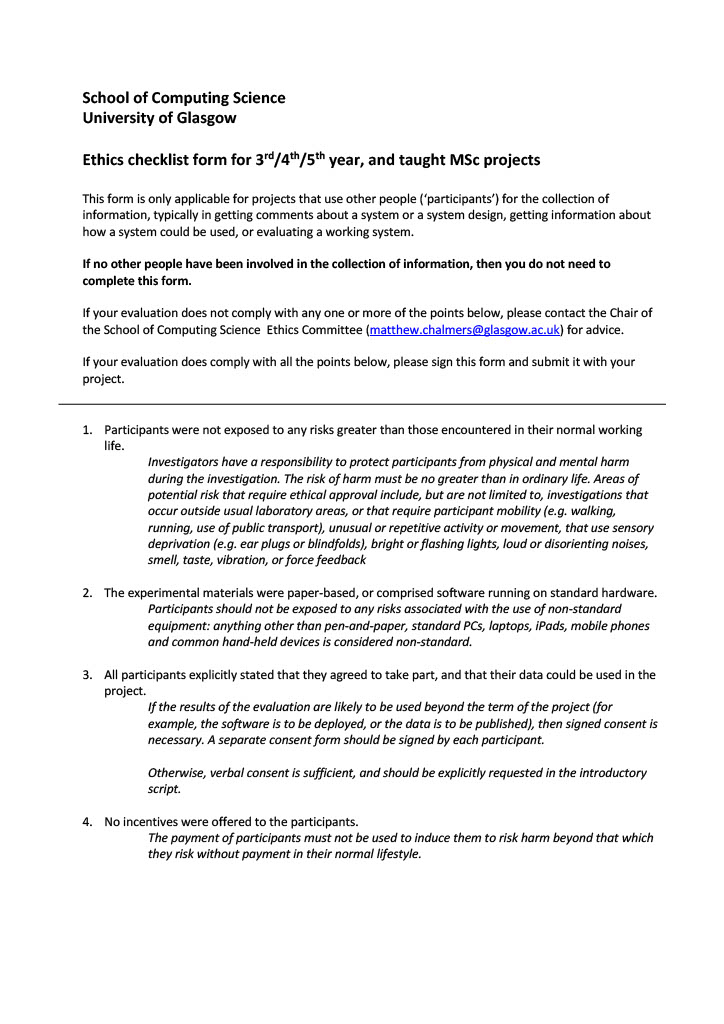
\includegraphics[width=0.95\linewidth]{images/Zsolt Takacs 2472886T Ethics Checklist1024_1.jpg}
    \caption{Page one of the approved ethics checklist}
    \label{fig:ethics_1} 
\end{figure}

\begin{figure}[H]
\centering
    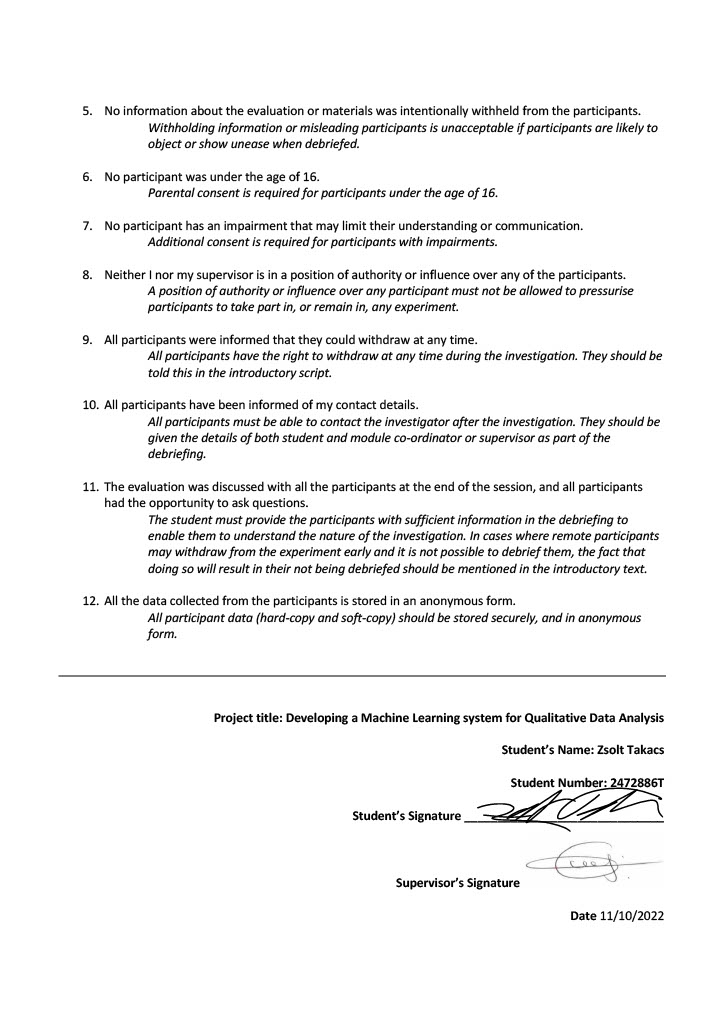
\includegraphics[width=0.95\linewidth]{images/Zsolt Takacs 2472886T Ethics Checklist1024_2.jpg}
    \caption{Page two of the approved ethics checklist}
    \label{fig:ethics_2} 
\end{figure}

\chapter{Activity Diagram}
\label{appendix:b}

\begin{figure}[H]
\centering
    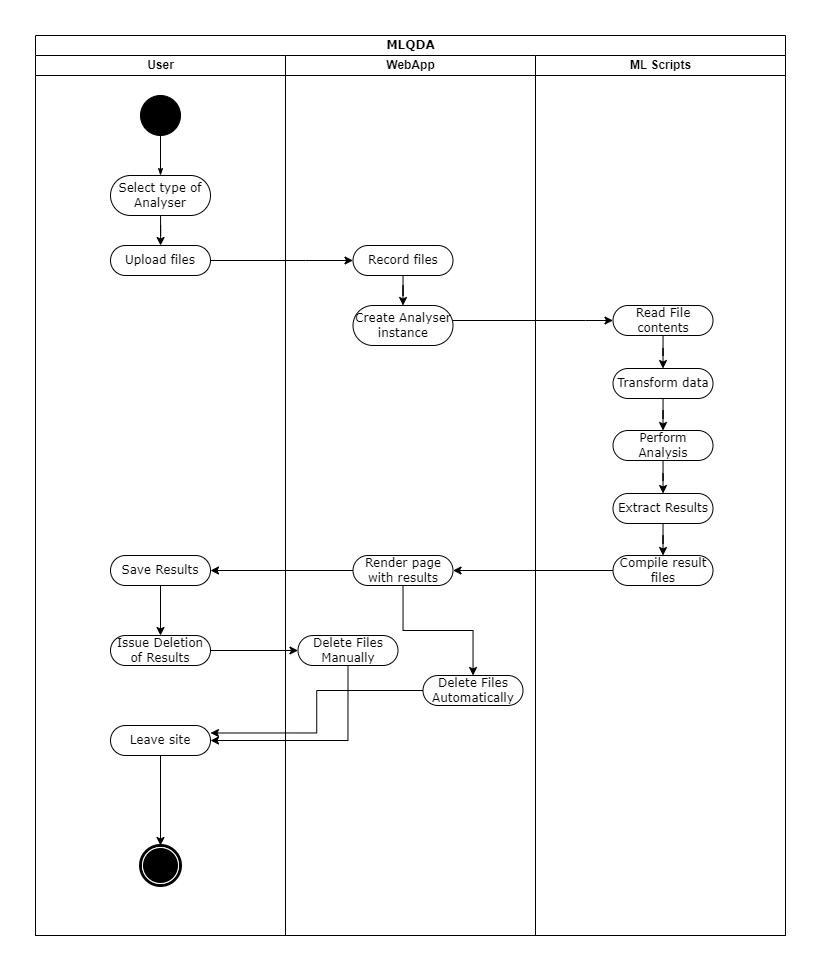
\includegraphics[width=0.95\linewidth]{images/mlqda_activity.drawio.png}
    \caption{Activity Diagram showing how a user would use the system to analyse their data. The diagram does not distinguish between different types of machine learning scripts. The exact steps involving the preparation and analysis of data might differ but should always end by producing a compiled set of results.}
    \label{fig:mlqda_activity} 
\end{figure}


\chapter{Wireframes}
\label{appendix:wireframes}
\begin{figure}[H]
\centering
    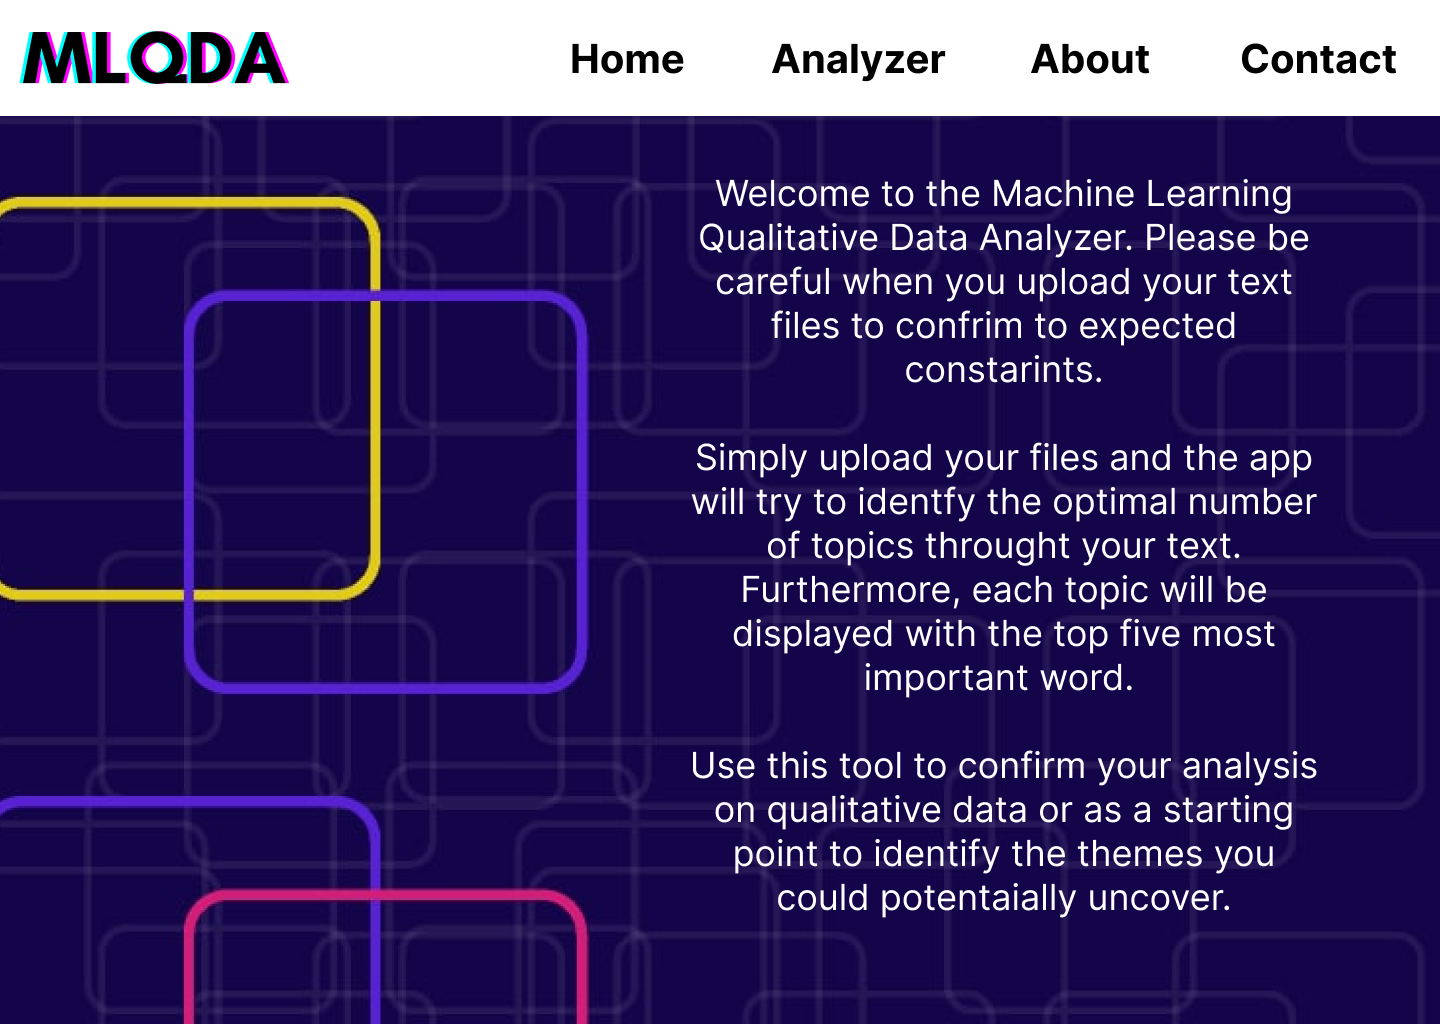
\includegraphics[width=0.95\linewidth]{images/Home.png}
    \caption{Wireframe displaying the home page.}
    \label{fig:wireframes_home} 
\end{figure}

\begin{figure}[H]
\centering
    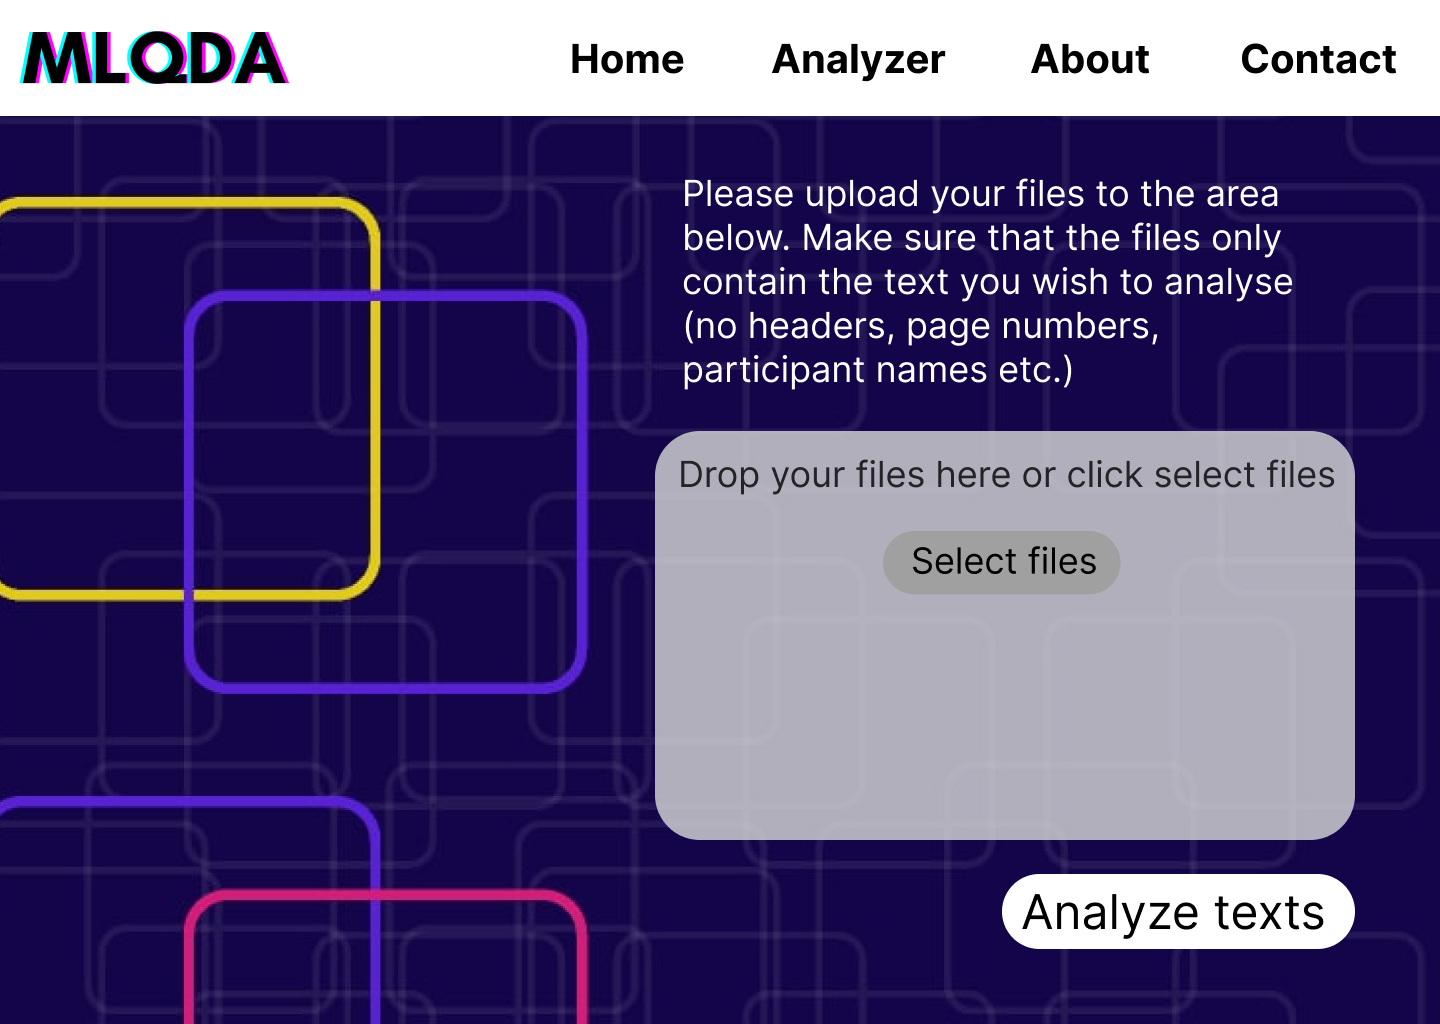
\includegraphics[width=0.95\linewidth]{images/Analyzer (start).png}
    \caption{Wireframe displaying the start page for an Analyser.}
    \label{fig:wireframes_analyser_start} 
\end{figure}

\begin{figure}[H]
\centering
    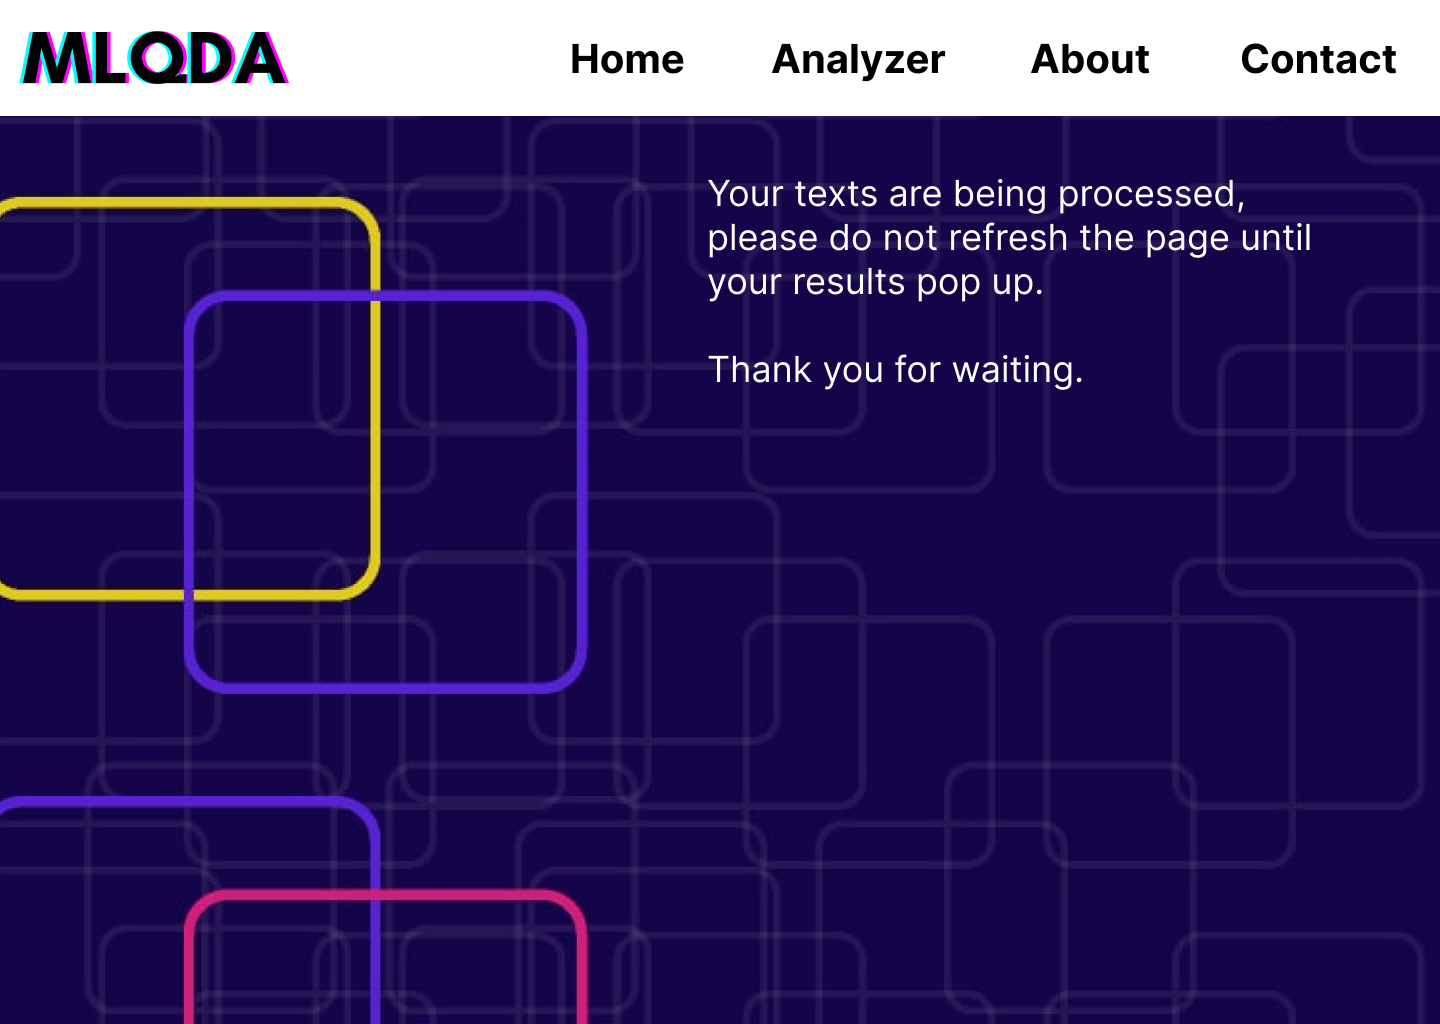
\includegraphics[width=0.95\linewidth]{images/Analyzer (process).png}
    \caption{Wireframe displaying placeholder while the analyser runs.}
    \label{fig:wireframes_placeholder} 
\end{figure}

\begin{figure}[H]
\centering
    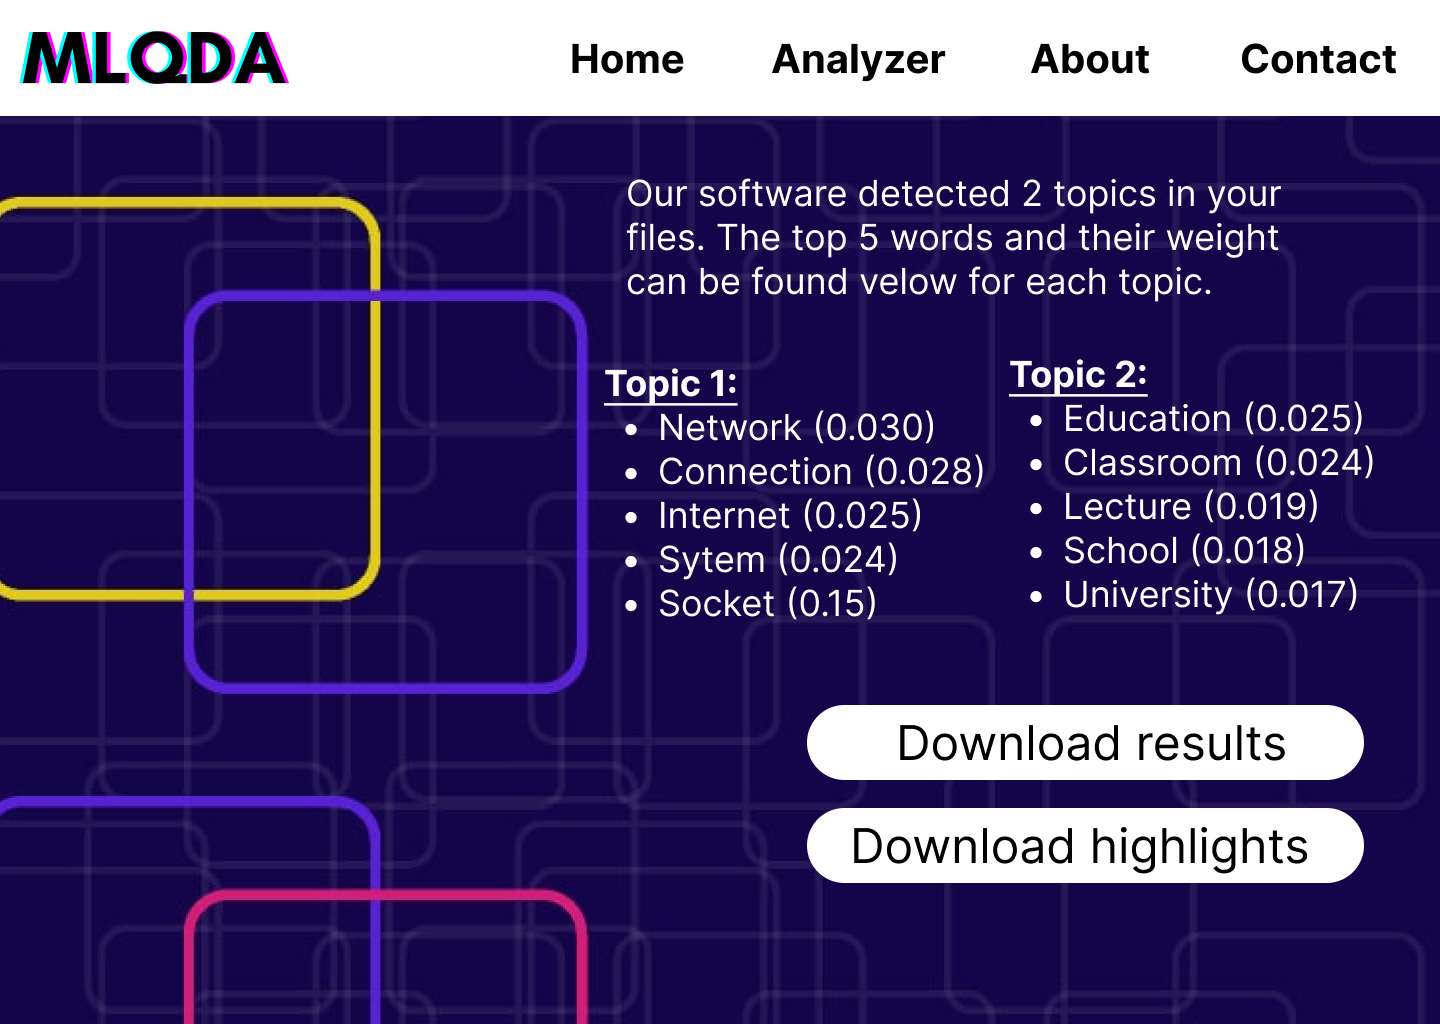
\includegraphics[width=0.95\linewidth]{images/Analyzer (results).png}
    \caption{Wireframe displaying the results page.}
    \label{fig:wireframes_results} 
\end{figure}

\begin{figure}[H]
\centering
    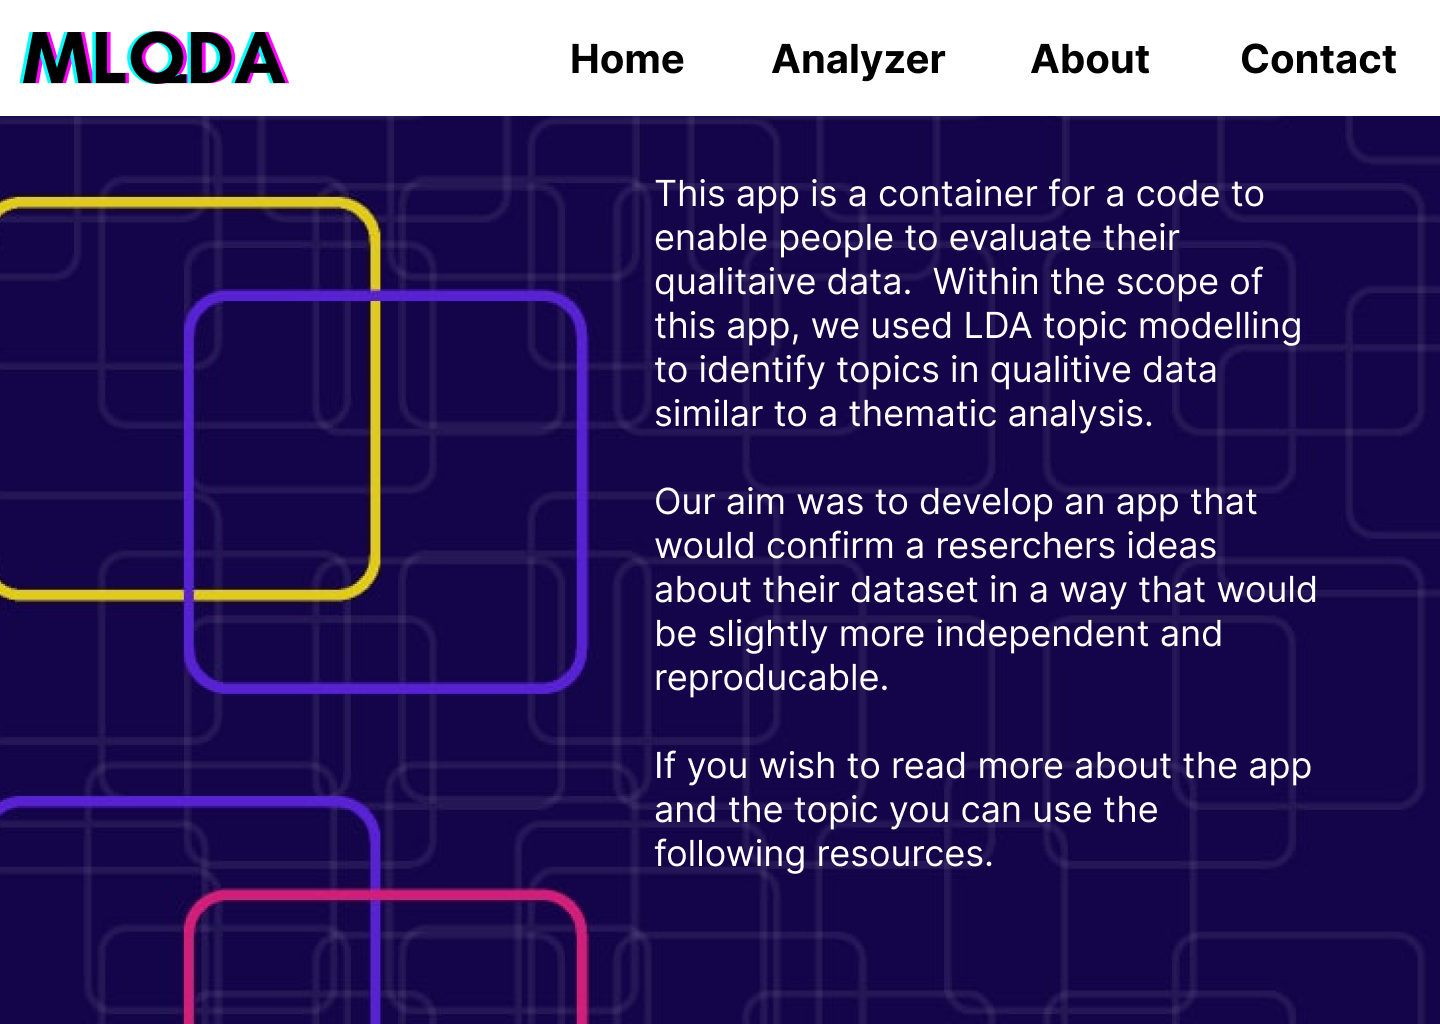
\includegraphics[width=0.95\linewidth]{images/About.png}
    \caption{Wireframe displaying the about page.}
    \label{fig:wireframes_about} 
\end{figure}

\begin{figure}[H]
\centering
    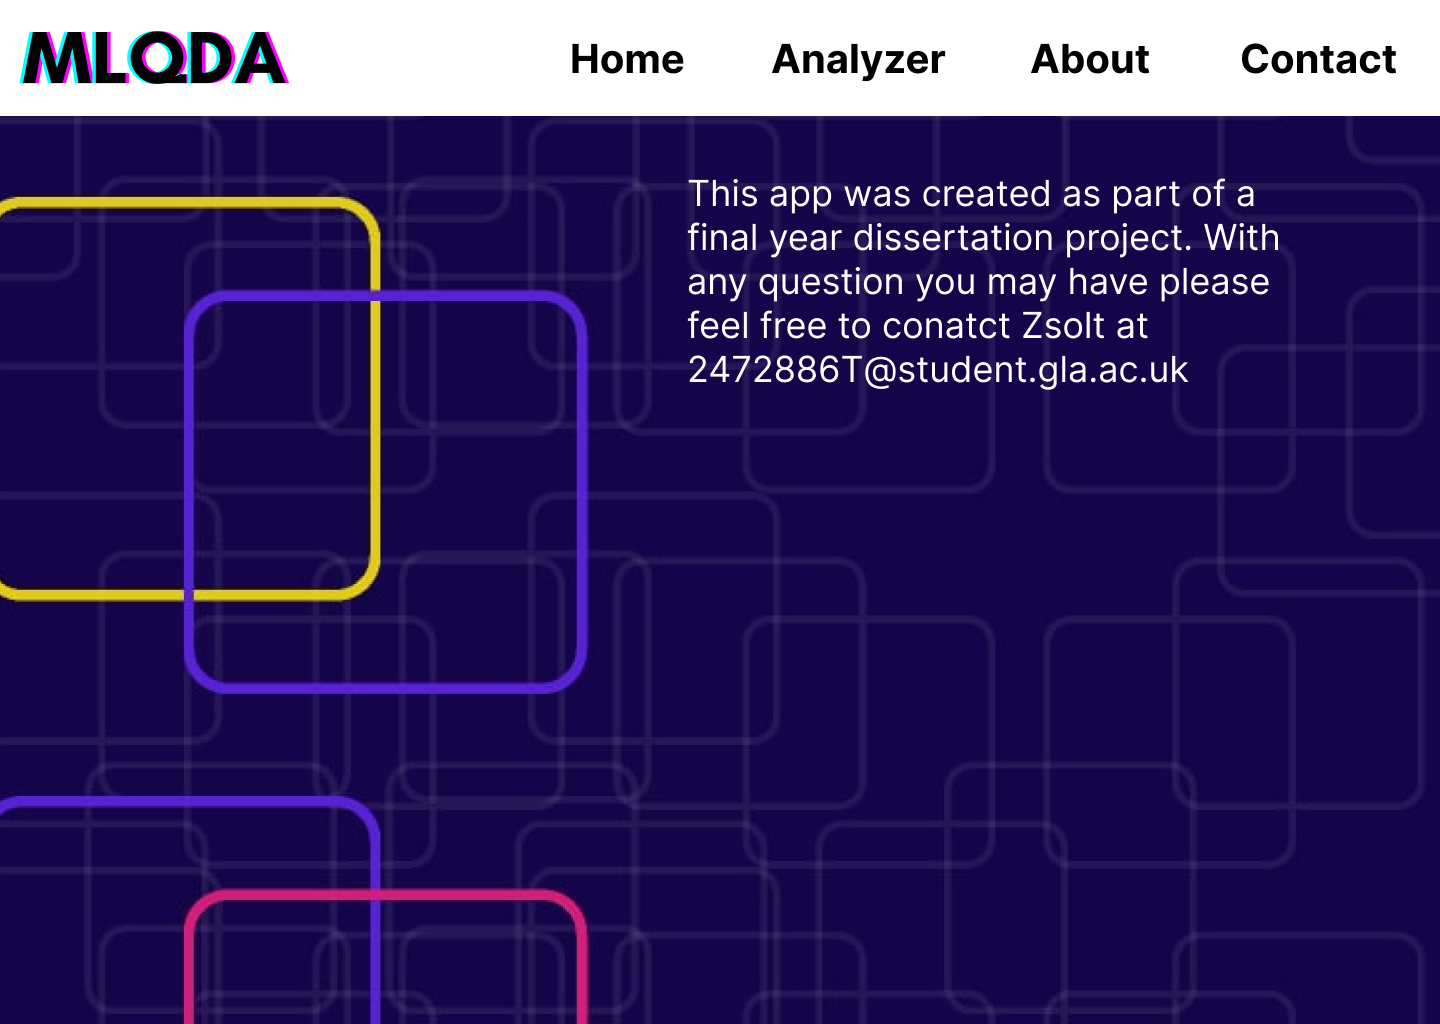
\includegraphics[width=0.95\linewidth]{images/Contact.png}
    \caption{Wireframe displaying the contact page.}
    \label{fig:wireframes_contact} 
\end{figure}

\chapter{Topic Modelling Workflow}
\label{appendix:tm_workflow}
To begin with, the system processes and transforms the original input texts into a format used in the topic modelling algorithm. First, the corpus is divided into single words to allow the system to clean it during the next step. The first cleaning step involves lemmatising the words and reducing them to their smallest grammatical form. This ensures that words with the same root will be identified as the same, no matter their grammatical form. The second step of cleaning the data filters out all stopwords from the corpus. Stopwords are part of a language that do not carry any meaning of content. Their primary function is to make sentences grammatically correct. As our model focuses on content, we can safely remove these words.

From the cleaned corpus, the system creates helper data structures. The first type of data structure is an N-gram, which represents word combinations to the degree of N. The current implementation supports bi-grams and tri-grams, meaning that two and three words following each other frequently will be identified as one term rather than three separate ones. When all bi-grams and tri-grams have been identified, the system converts the corpus represented as a list of words into a dictionary-like id2word object. Id2word objects are in essential dictionaries to map a unique id to a word. Finally, the id2word objects are converted into a BoW (Bag-of-Words) object, a grouped and summed version of the previous structure based on the original document and the count for each unique term. By this point, the data is completely illegible to the human eye. However, it is perfectly formatted to run an LDA Topic Modelling script.

From the original corpus and the id2word structure, a TfidfModel is created. TF-IDF scores measure the importance of a term within the corpus. For the script to detect more distinct topics, all terms with a lower TF-IDF score than the median are removed. Using the filtered id2words and the BoW structures, the LDA model randomly allocates terms to a pre-set number of topics throughout a pre-set number of iterations. Each model with a different number of topics is run parallel to speed up the process. The best model is selected based on the highest Coherence score, which measures the internal validity of the model. The best model returns the top 10 words connected to the proposed underlying themes. The themes are unnamed; hence they need human deduction to infer a name for the theme. The script saves these results as a dictionary to allow later compilation of all result files.

\chapter{Graphical User Interface - GUI}
\label{appendix:gui}

\begin{figure}[H]
\centering
    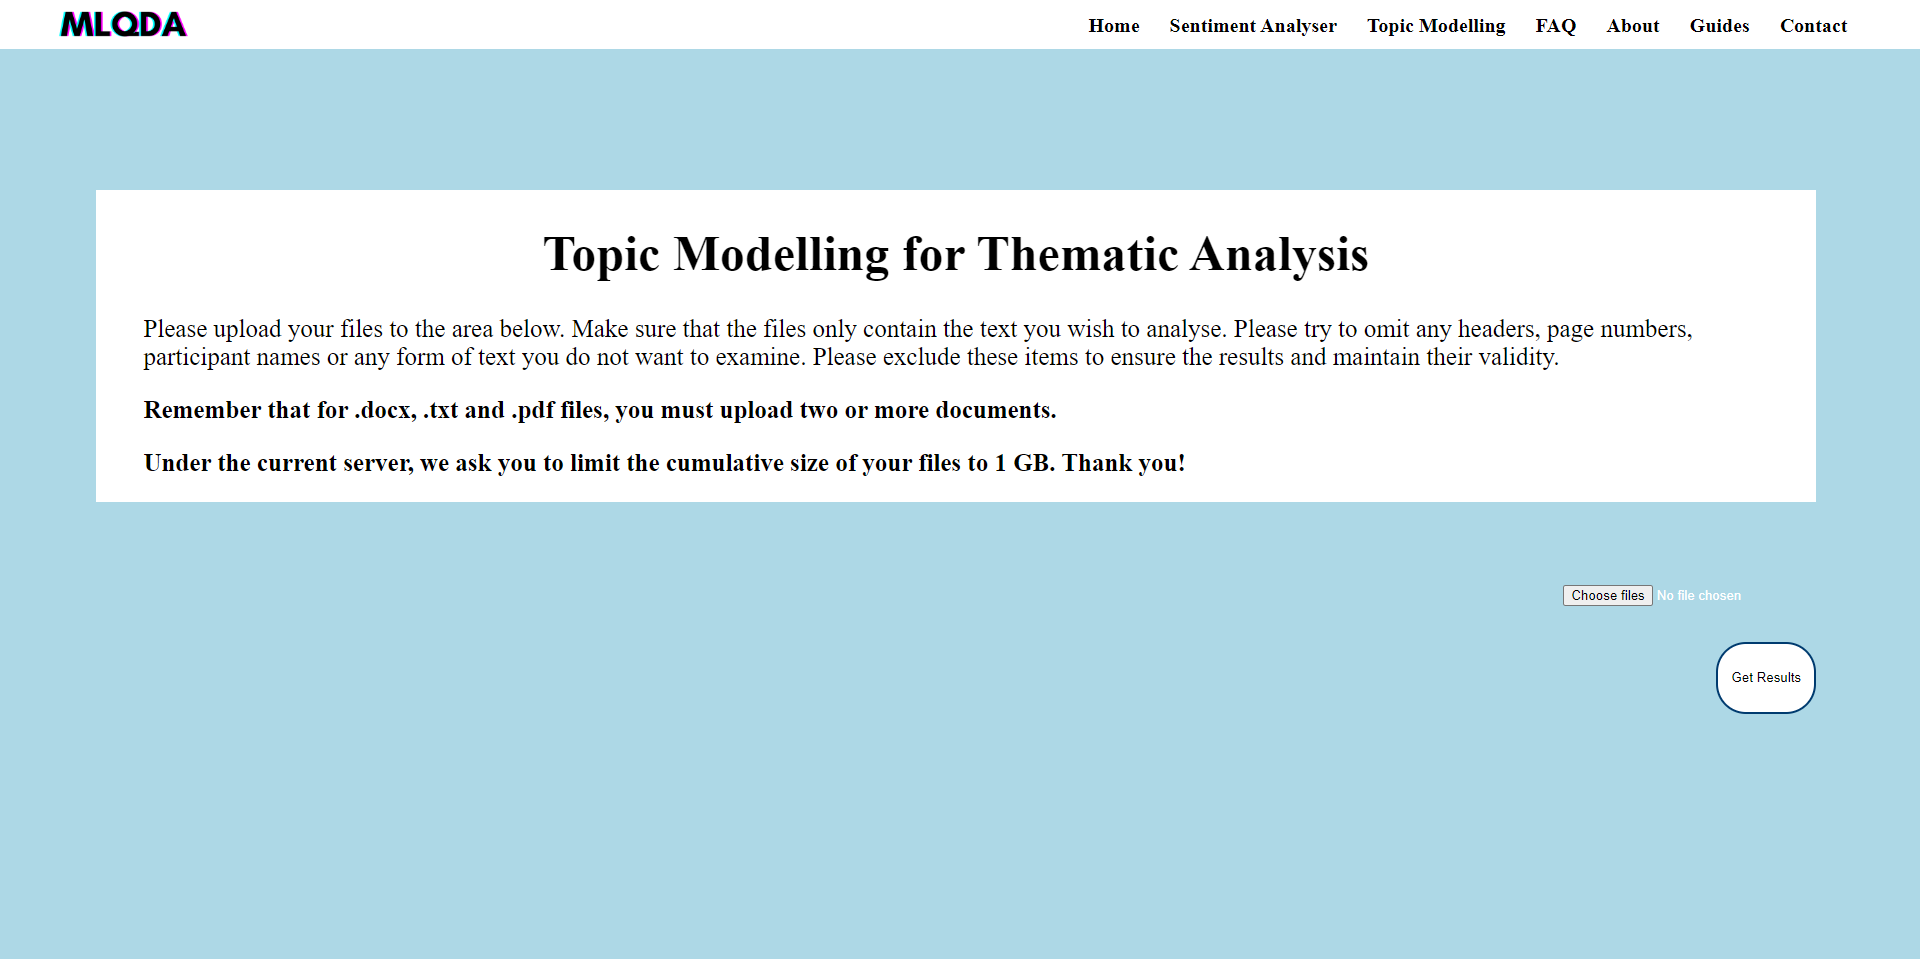
\includegraphics[width=0.95\linewidth]{images/tm_start.png}
    \caption{Start page for Topic Modelling}
    \label{fig:mlqda_tm_start} 
\end{figure}

\begin{figure}[H]
\centering
    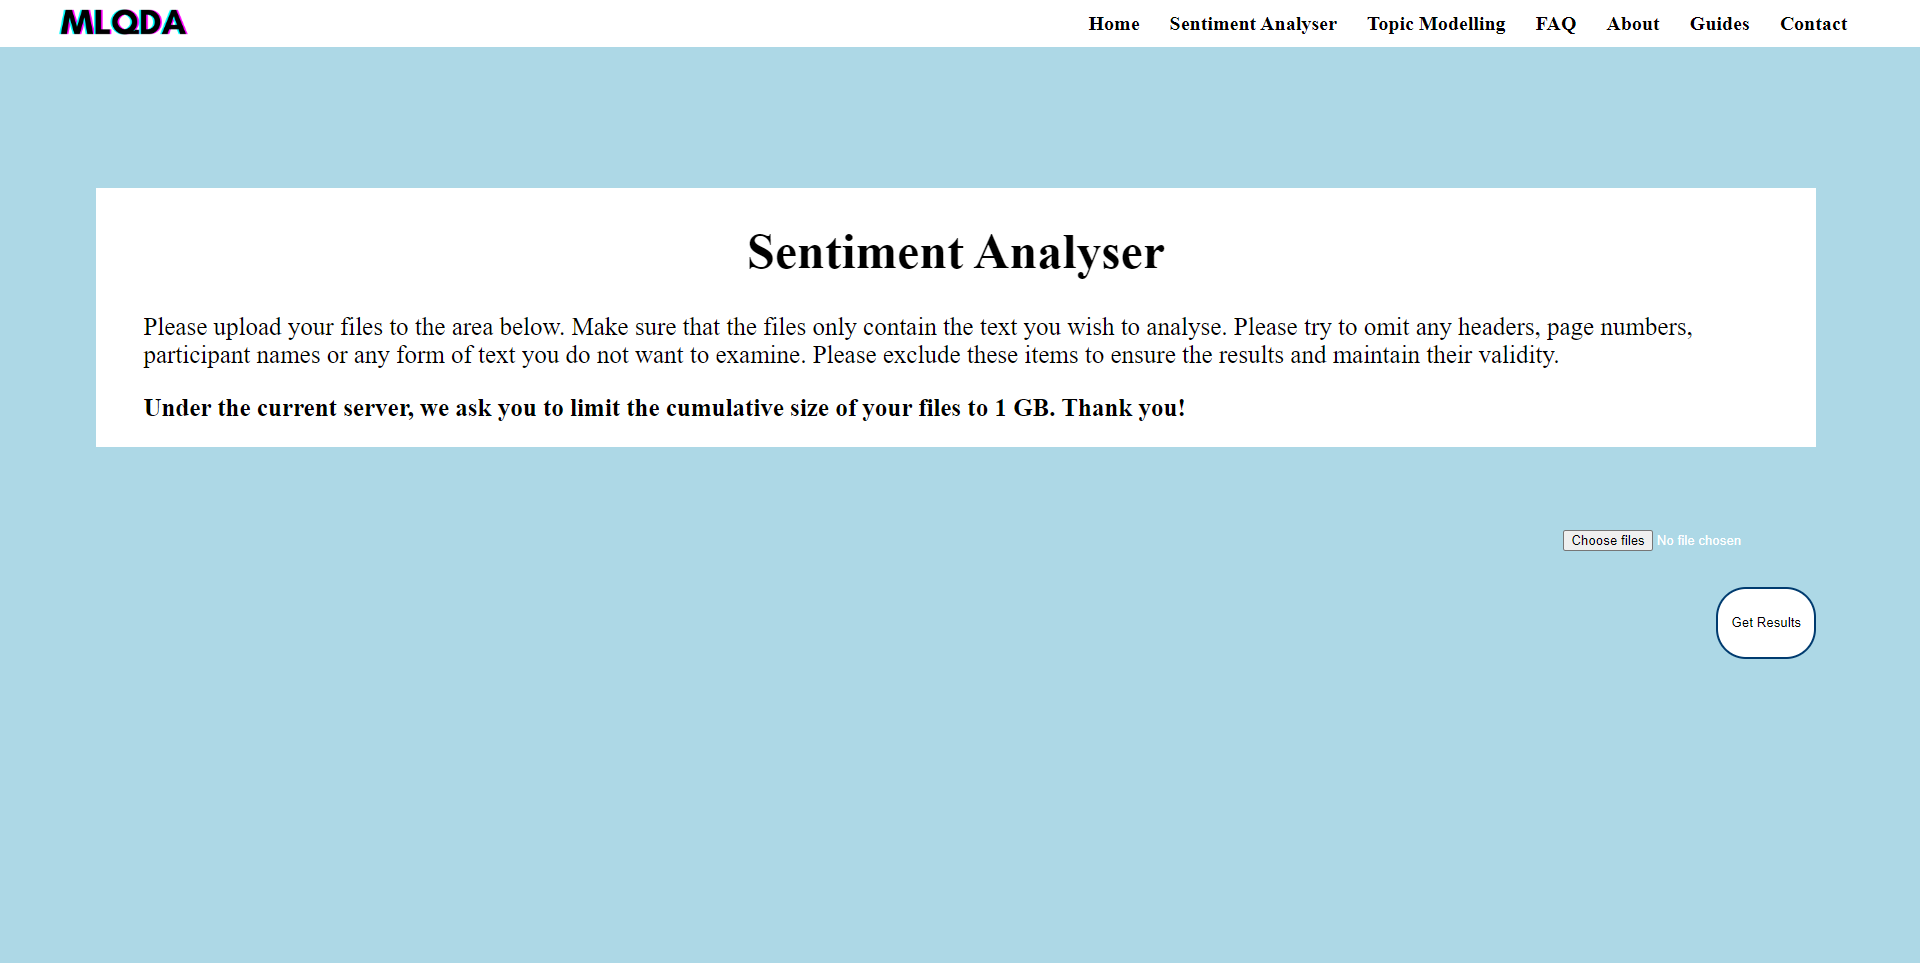
\includegraphics[width=0.95\linewidth]{images/sa_start.png}
    \caption{Start page for Sentiment Analysis}
    \label{fig:mlqda_sa_start} 
\end{figure}

\begin{figure}[H]
    \centering
    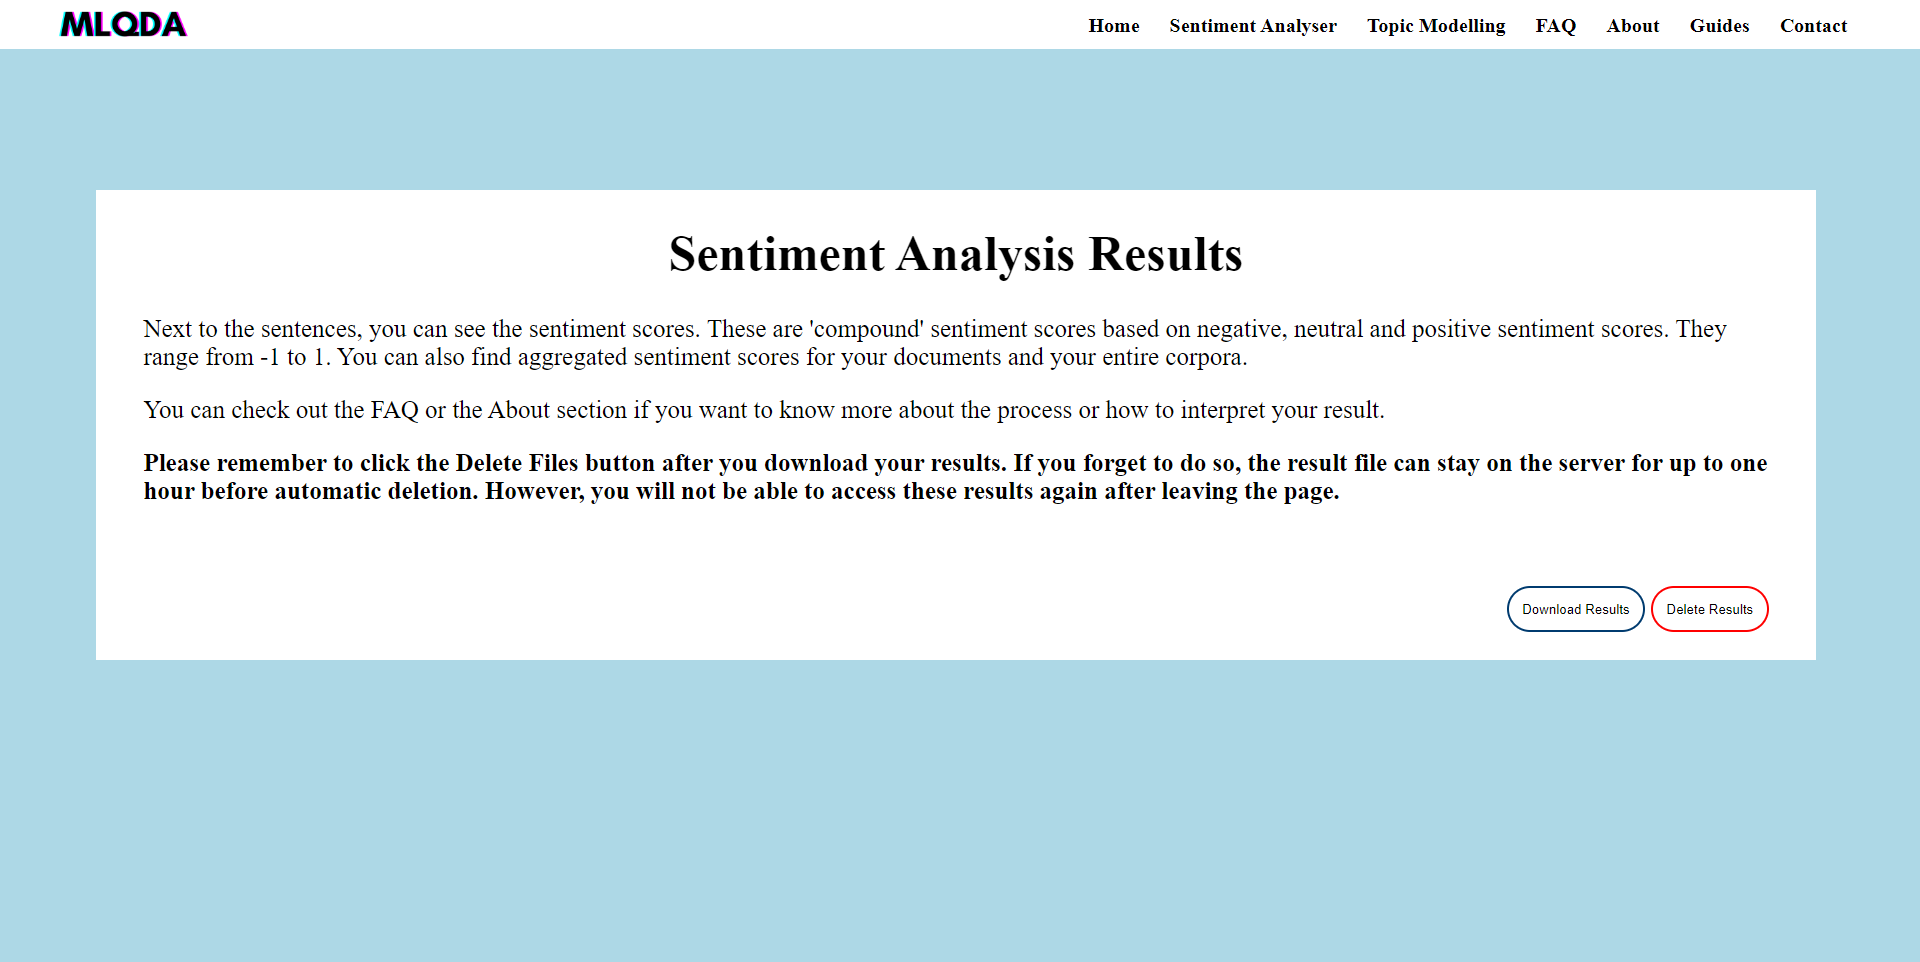
\includegraphics[width=0.95\linewidth]{images/sa_results.png}
    \caption{Results page for Sentiment Analysis}
    \label{fig:sa_results} 
\end{figure}

\begin{figure}[H]
    \centering
    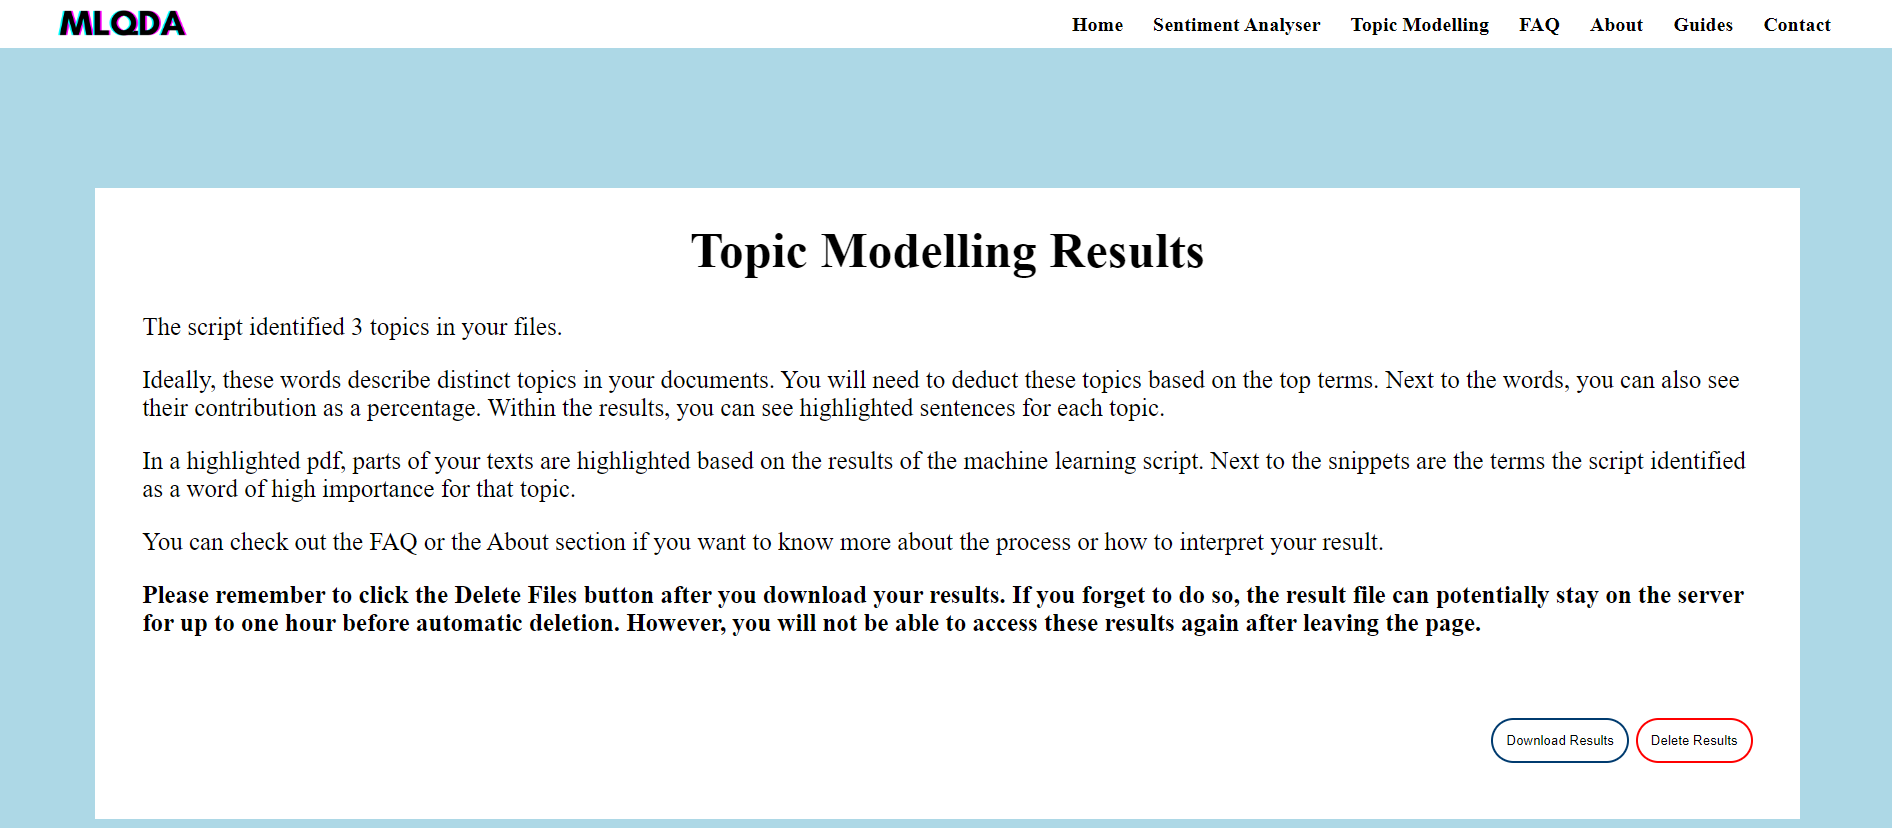
\includegraphics[width=0.95\linewidth]{images/tm_results_1.png}
    \caption{Results page for Topic Modelling}
    \label{fig:tm_results_1} 
\end{figure}

\begin{figure}[H]
    \centering
    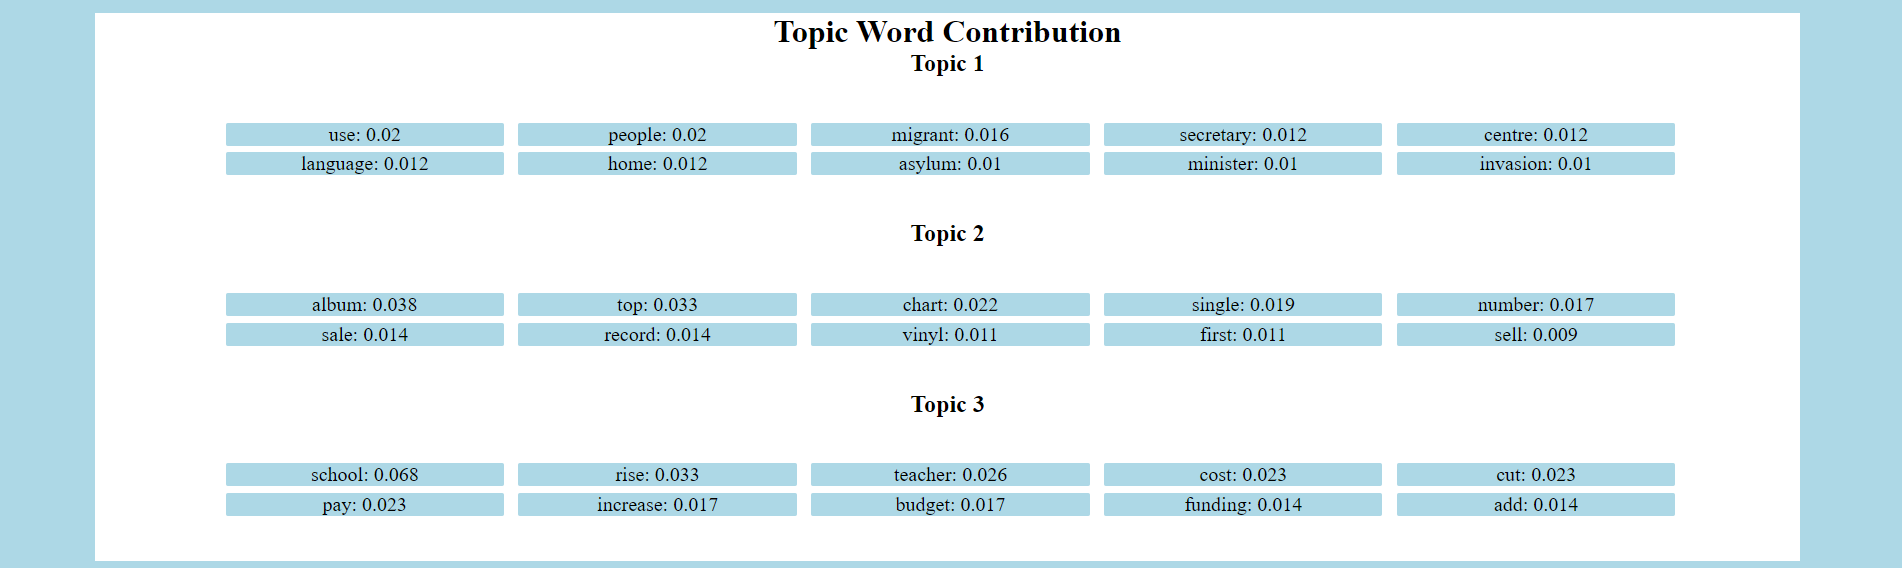
\includegraphics[width=0.95\linewidth]{images/tm_results_2.png}
    \caption{Results page for Topic Modelling}
    \label{fig:tm_results_2} 
\end{figure}


 \chapter{Final User Evaluation Questionnaire Example}
 \label{appendix:user_eval}
 \section{Demographic background}
 The following demographic questions were included to measure familiarity with the used technologies:
 \begin{enumerate}
     \item I am familiar with different qualitative data analysis methods.
     \item I am familiar with Sentiment Analysis.
     \item I am familiar with Thematic Analysis.
     \item I am familiar with Topic Modelling.
 \end{enumerate}

 \section{User Tasks}
 The follwoing four user tasks were asked to be performed by the users:
 \begin{enumerate}
     \item Please try to find information on how to prepare your files before uploading them to the system.
     \item Please try to find information on how the Topic Modelling script processes your files.
     \item Please perform a Sentiment Analysis on the provided files using the site.
     \item Please perform a Thematic Analysis on the provided files using the site.
 \end{enumerate}

 \section{System specific questions}
 The following questions were asked to measure the usability of this specific system:

Please indicate on the following scale how much you agree with the
following statements (1-5):
\begin{enumerate}
    \item While completing the tasks, I referred to the FAQ, Guide and/or About sections
    \item While completing the tasks, I found the information on the FAQ page useful.
    \item While completing the tasks, I found the information on the About page useful.
    \item While completing the tasks, I found the information on the Guide page useful.
    \item I found the Sentiment Analysis results clear and useful.
    \item I found the Thematic Analysis results based on Topic Modelling clear and useful
    \item I found that the site offers an adequate amount of information for users about the applied machinelearning techniques.
    \item I would find updating the results manually an excellent addition to the system.
\end{enumerate}
 
\section{System Usability Scale}
The System Usability Scale was developed by \cite{brooke1996sus} and it measures agreement on a Likert scale of five on these ten statements:

On a scale of 1-5, how much do you agree with the following
statements? (1 - Strongly Disagree; 5 - Strongly Agree)
\begin{enumerate}
    \item I think that I would like to use this system frequently.
    \item I found the system unnecessarily complex.
    \item I thought the system was easy to use.
    \item I think that I would need the support of a technical person to be able to use this system.
    \item I found the various functions in this system were well integrated.
    \item I thought there was too much inconsistency in this system.
    \item I would imagine that most people would learn to use this system very quickly.
    \item I found the system very cumbersome to use.
    \item I felt very confident using the system.
    \item I needed to learn a lot of things before I could get going with this system.
\end{enumerate}

\section{Comments and suggestions}

\begin{enumerate}
    \item Do you have any comments about the system after using it?
    \item Do you have any suggestions on how to improve the system?
\end{enumerate}


 \chapter{Final User Evaluation Results}
 \label{appendix:eval_results}

 \section{Visualisation of Demographic Data}

 \begin{figure}[H]
    \centering
    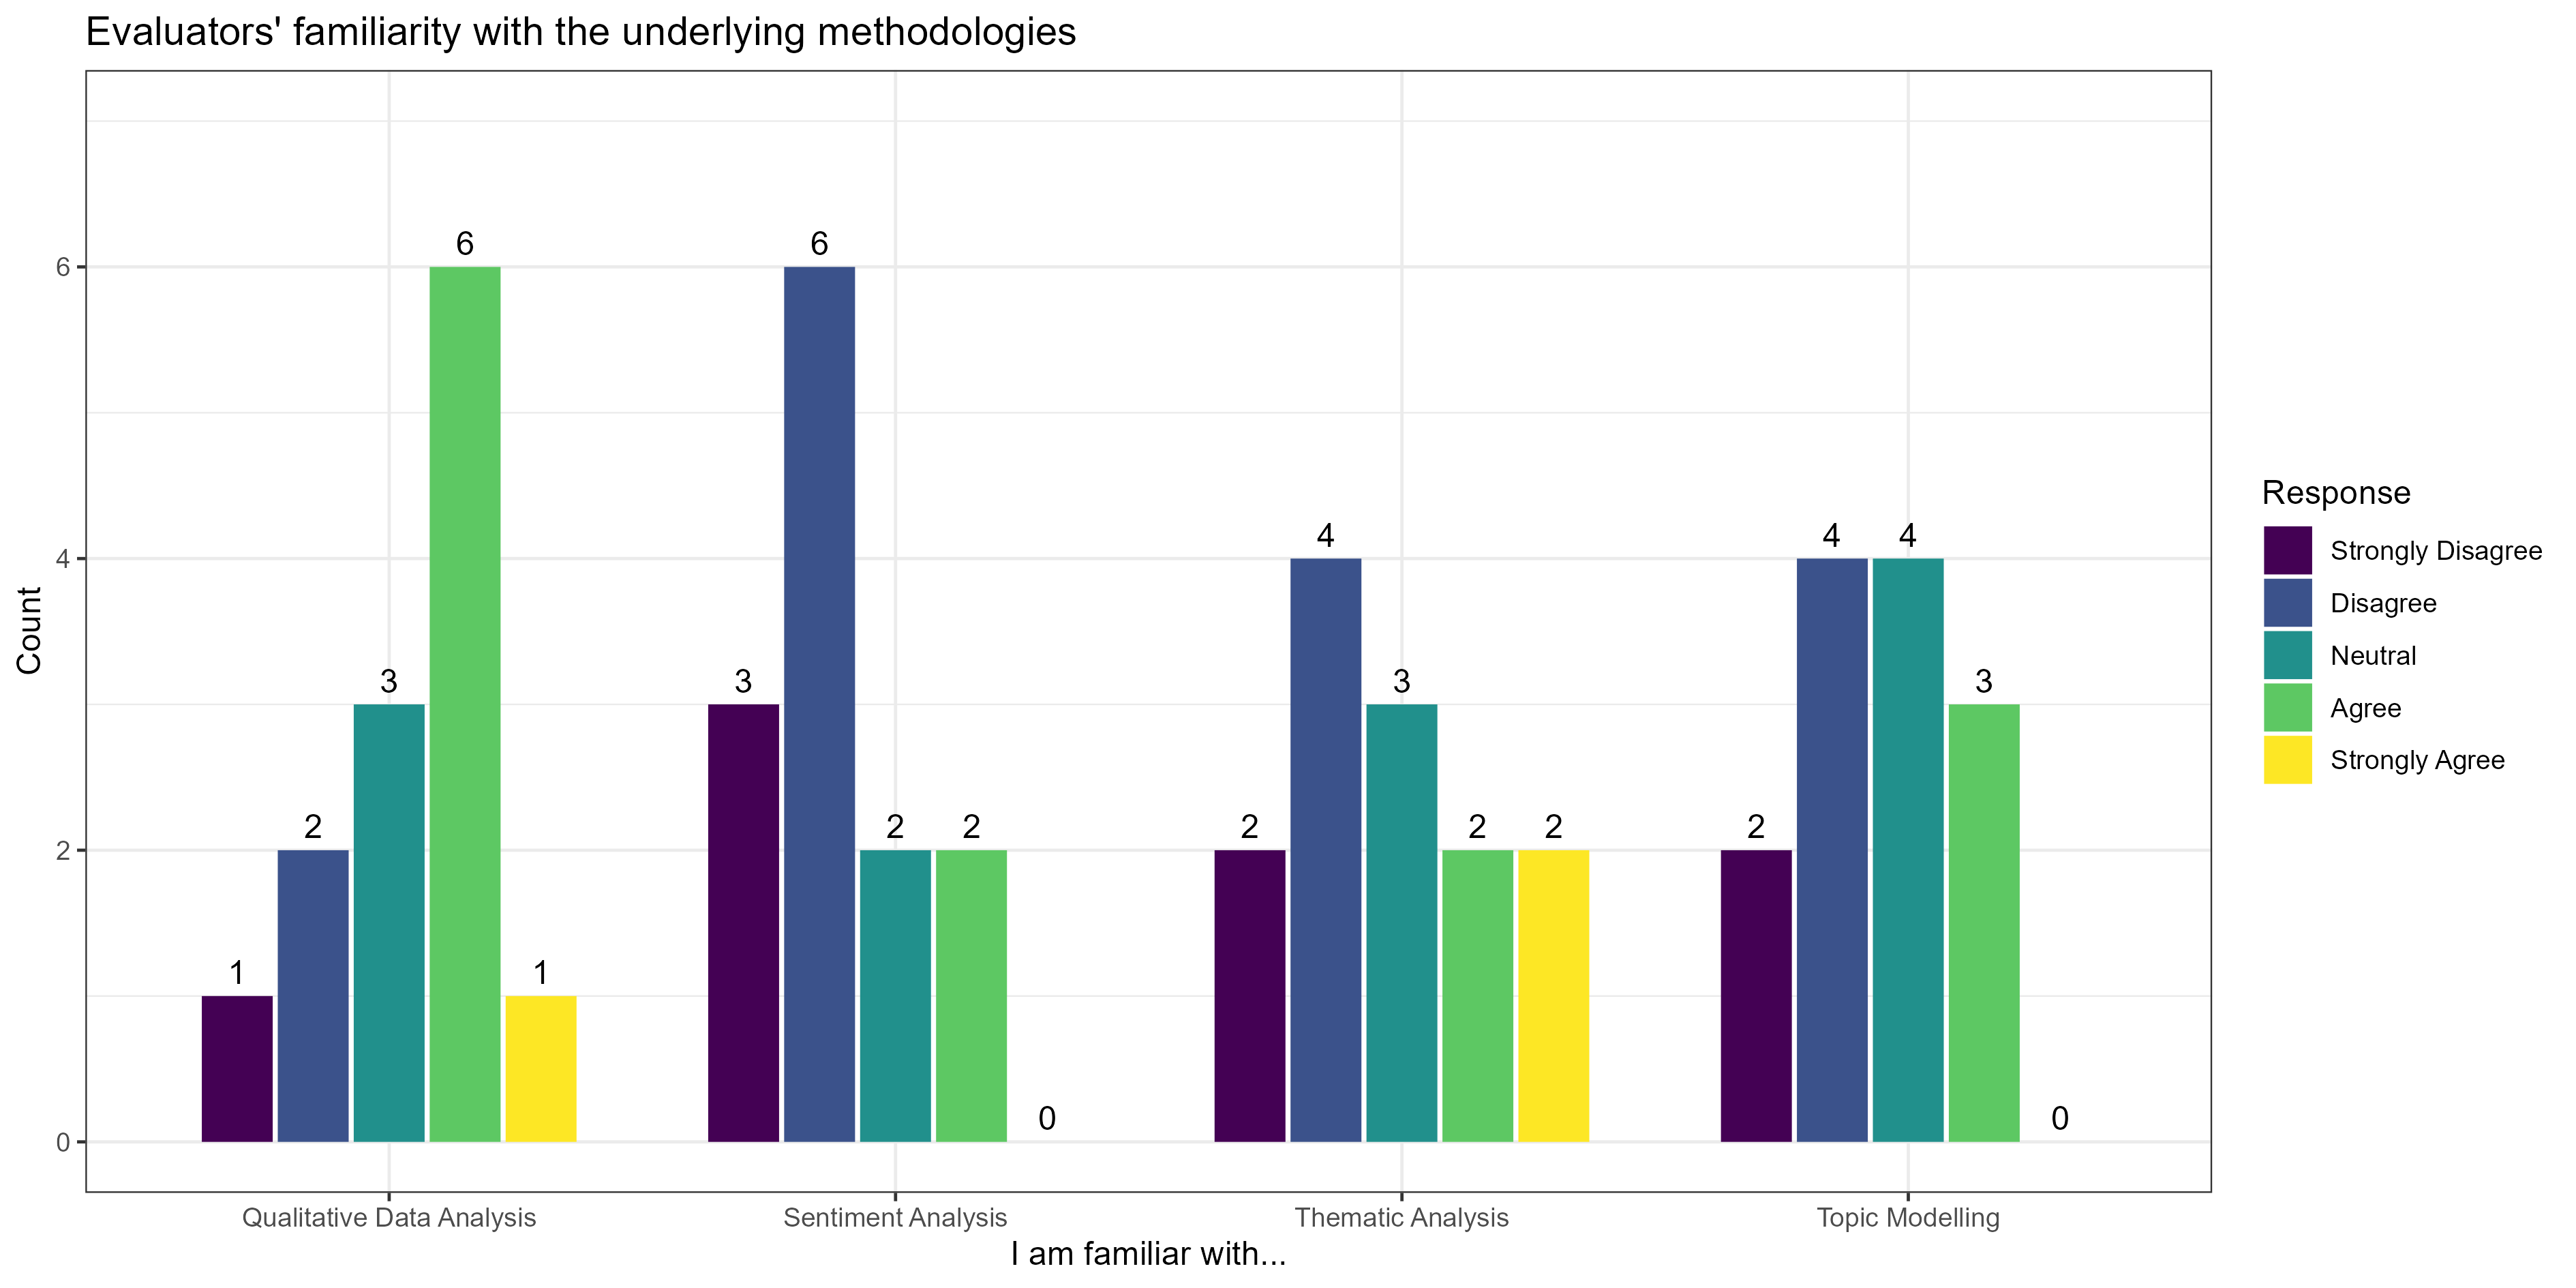
\includegraphics[width=1\linewidth]{images/demographics.png}
    \caption{Visualisation of Demographic Data}
    \label{fig:demographics_visual} 
\end{figure}

 \section{Visualisation of System Specific Questions}
  \begin{figure}[H]
    \centering
    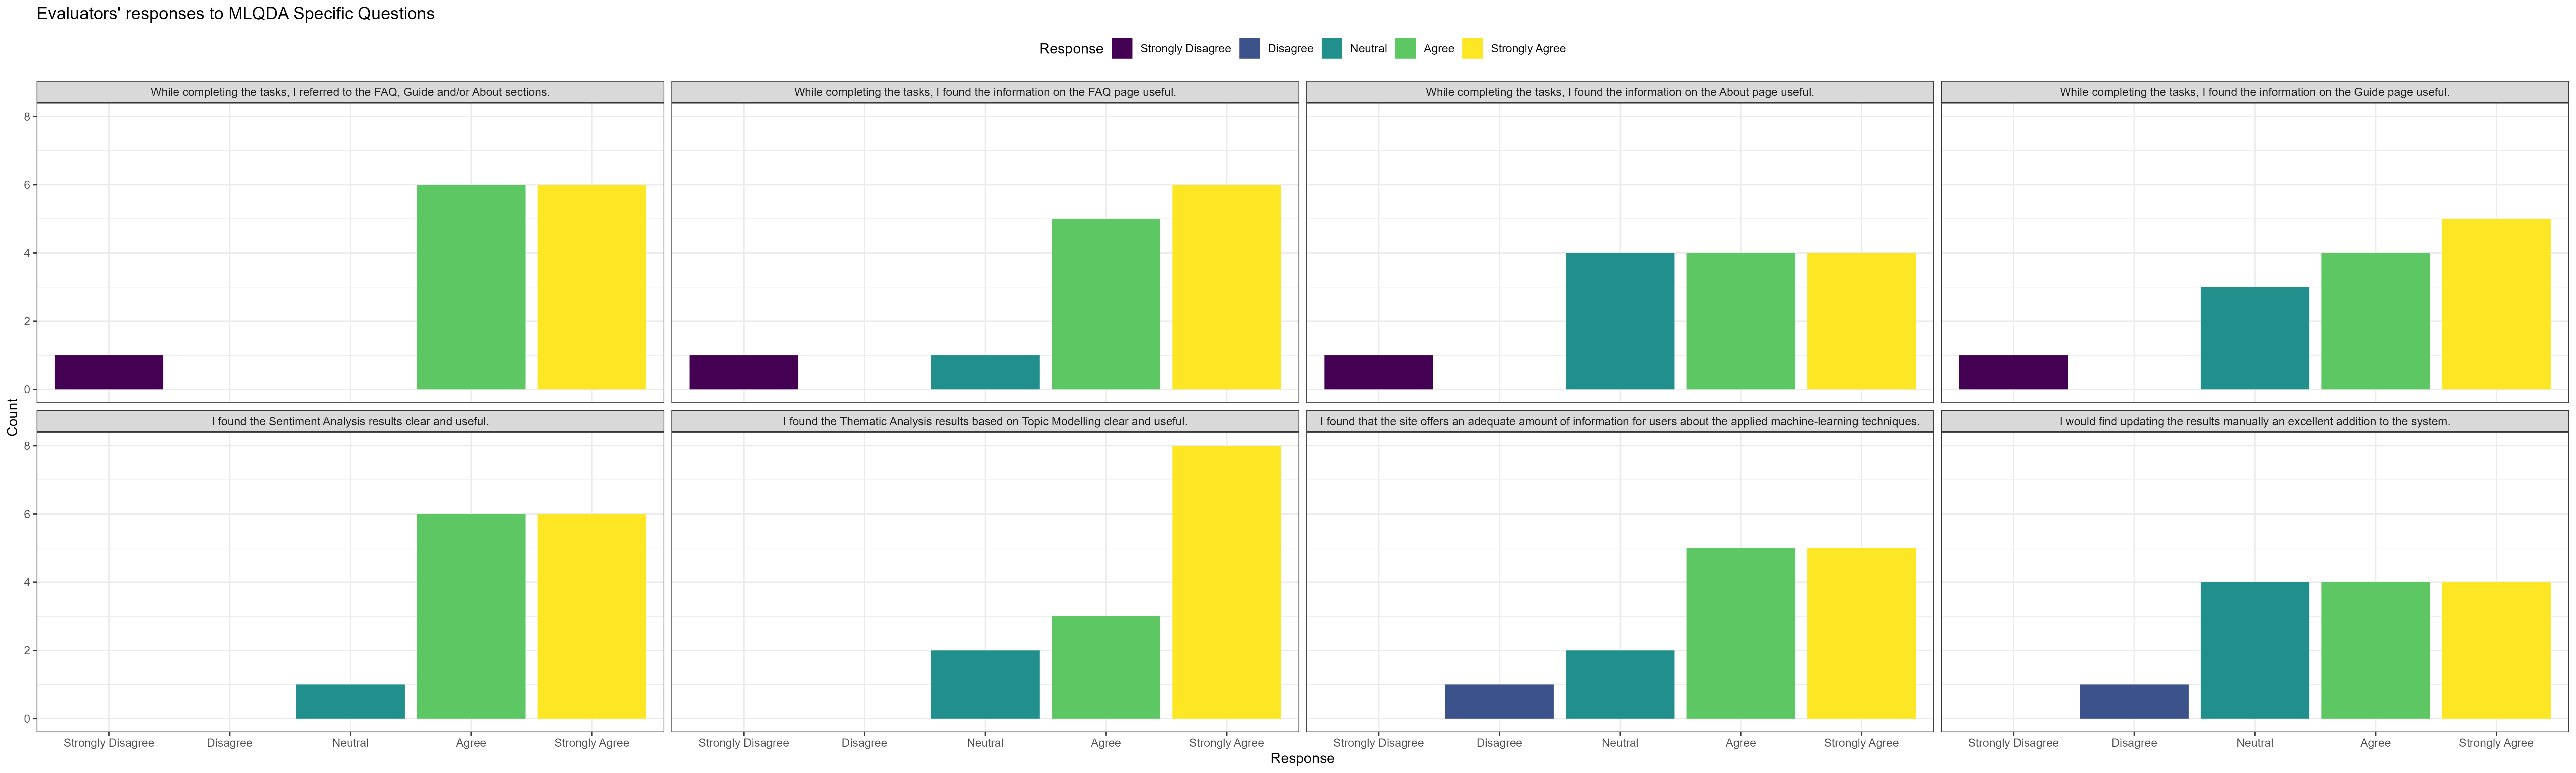
\includegraphics[width=550pt, angle=90]{images/system_specific_res.png}
    \caption{Visualisation of System Specific Questions}
    \label{fig:system_specific_visuals} 
\end{figure}

 \section{Visualisation for SUS scores}

 \begin{figure}[H]
    \centering
    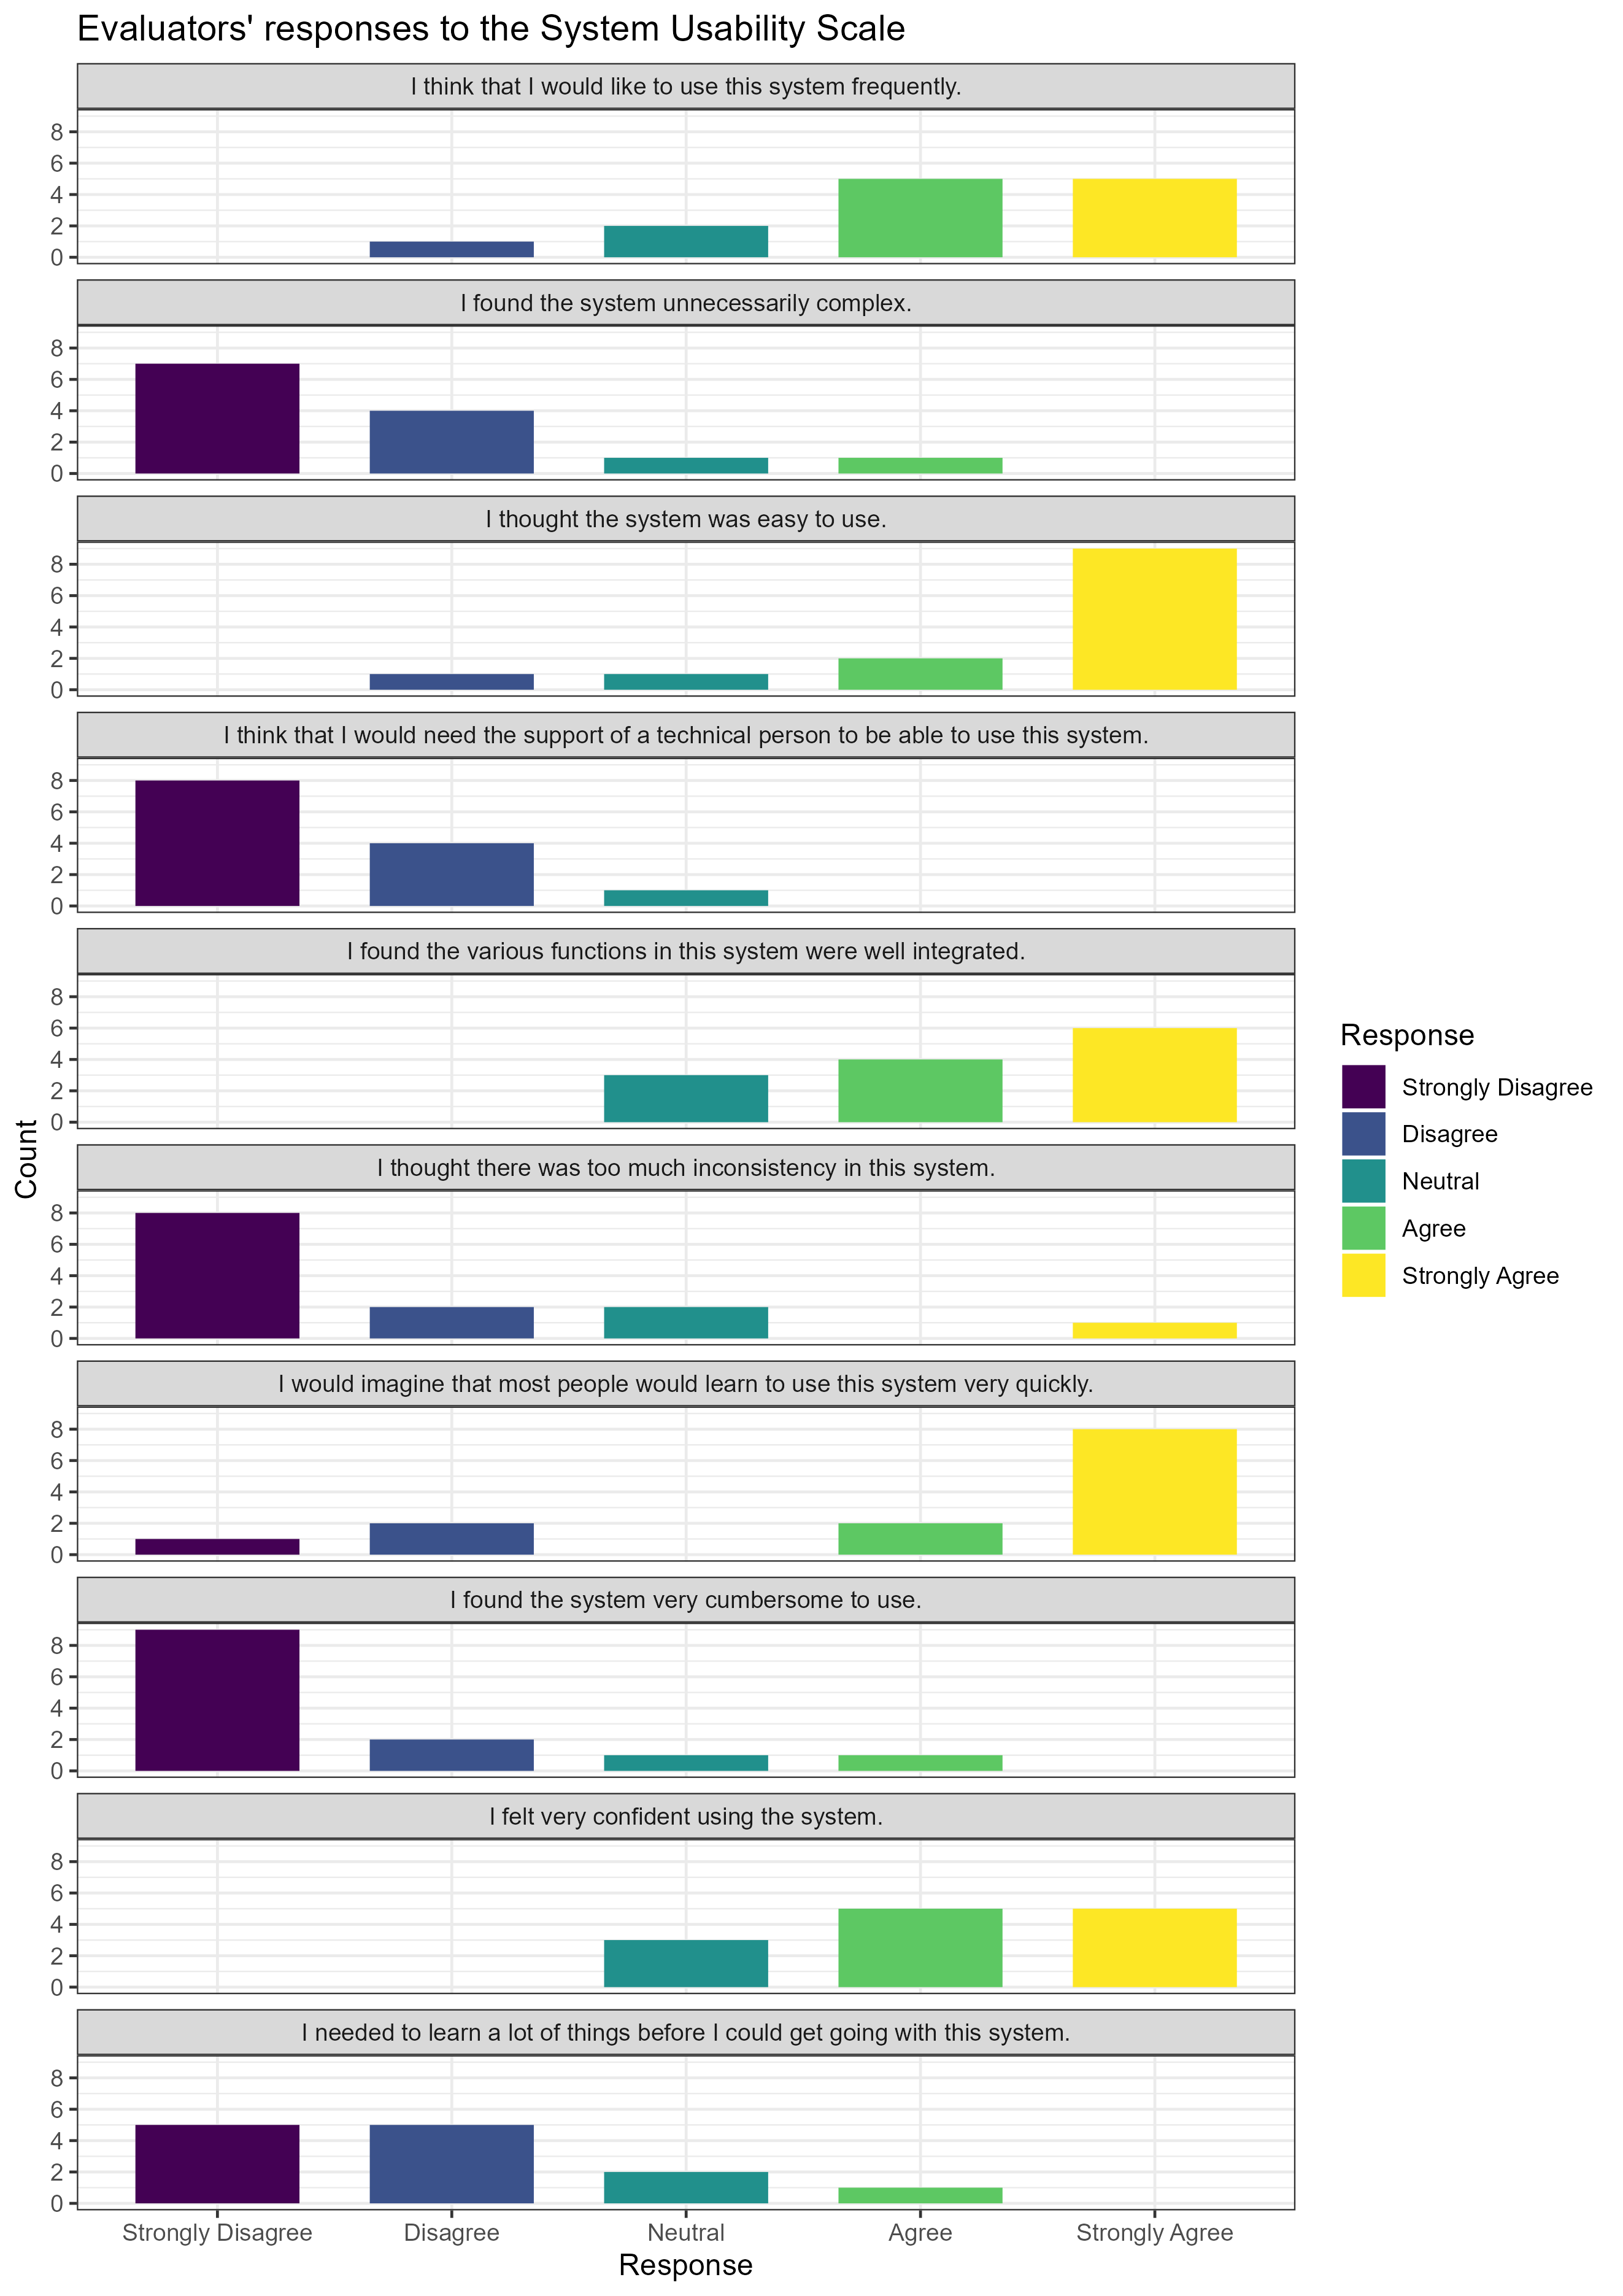
\includegraphics[width=1\linewidth]{images/sus_count_res.png}
    \caption{Visualisation of responses to individual SUS items}
    \label{fig:sus_items_visual} 
\end{figure}

 \begin{figure}[H]
    \centering
    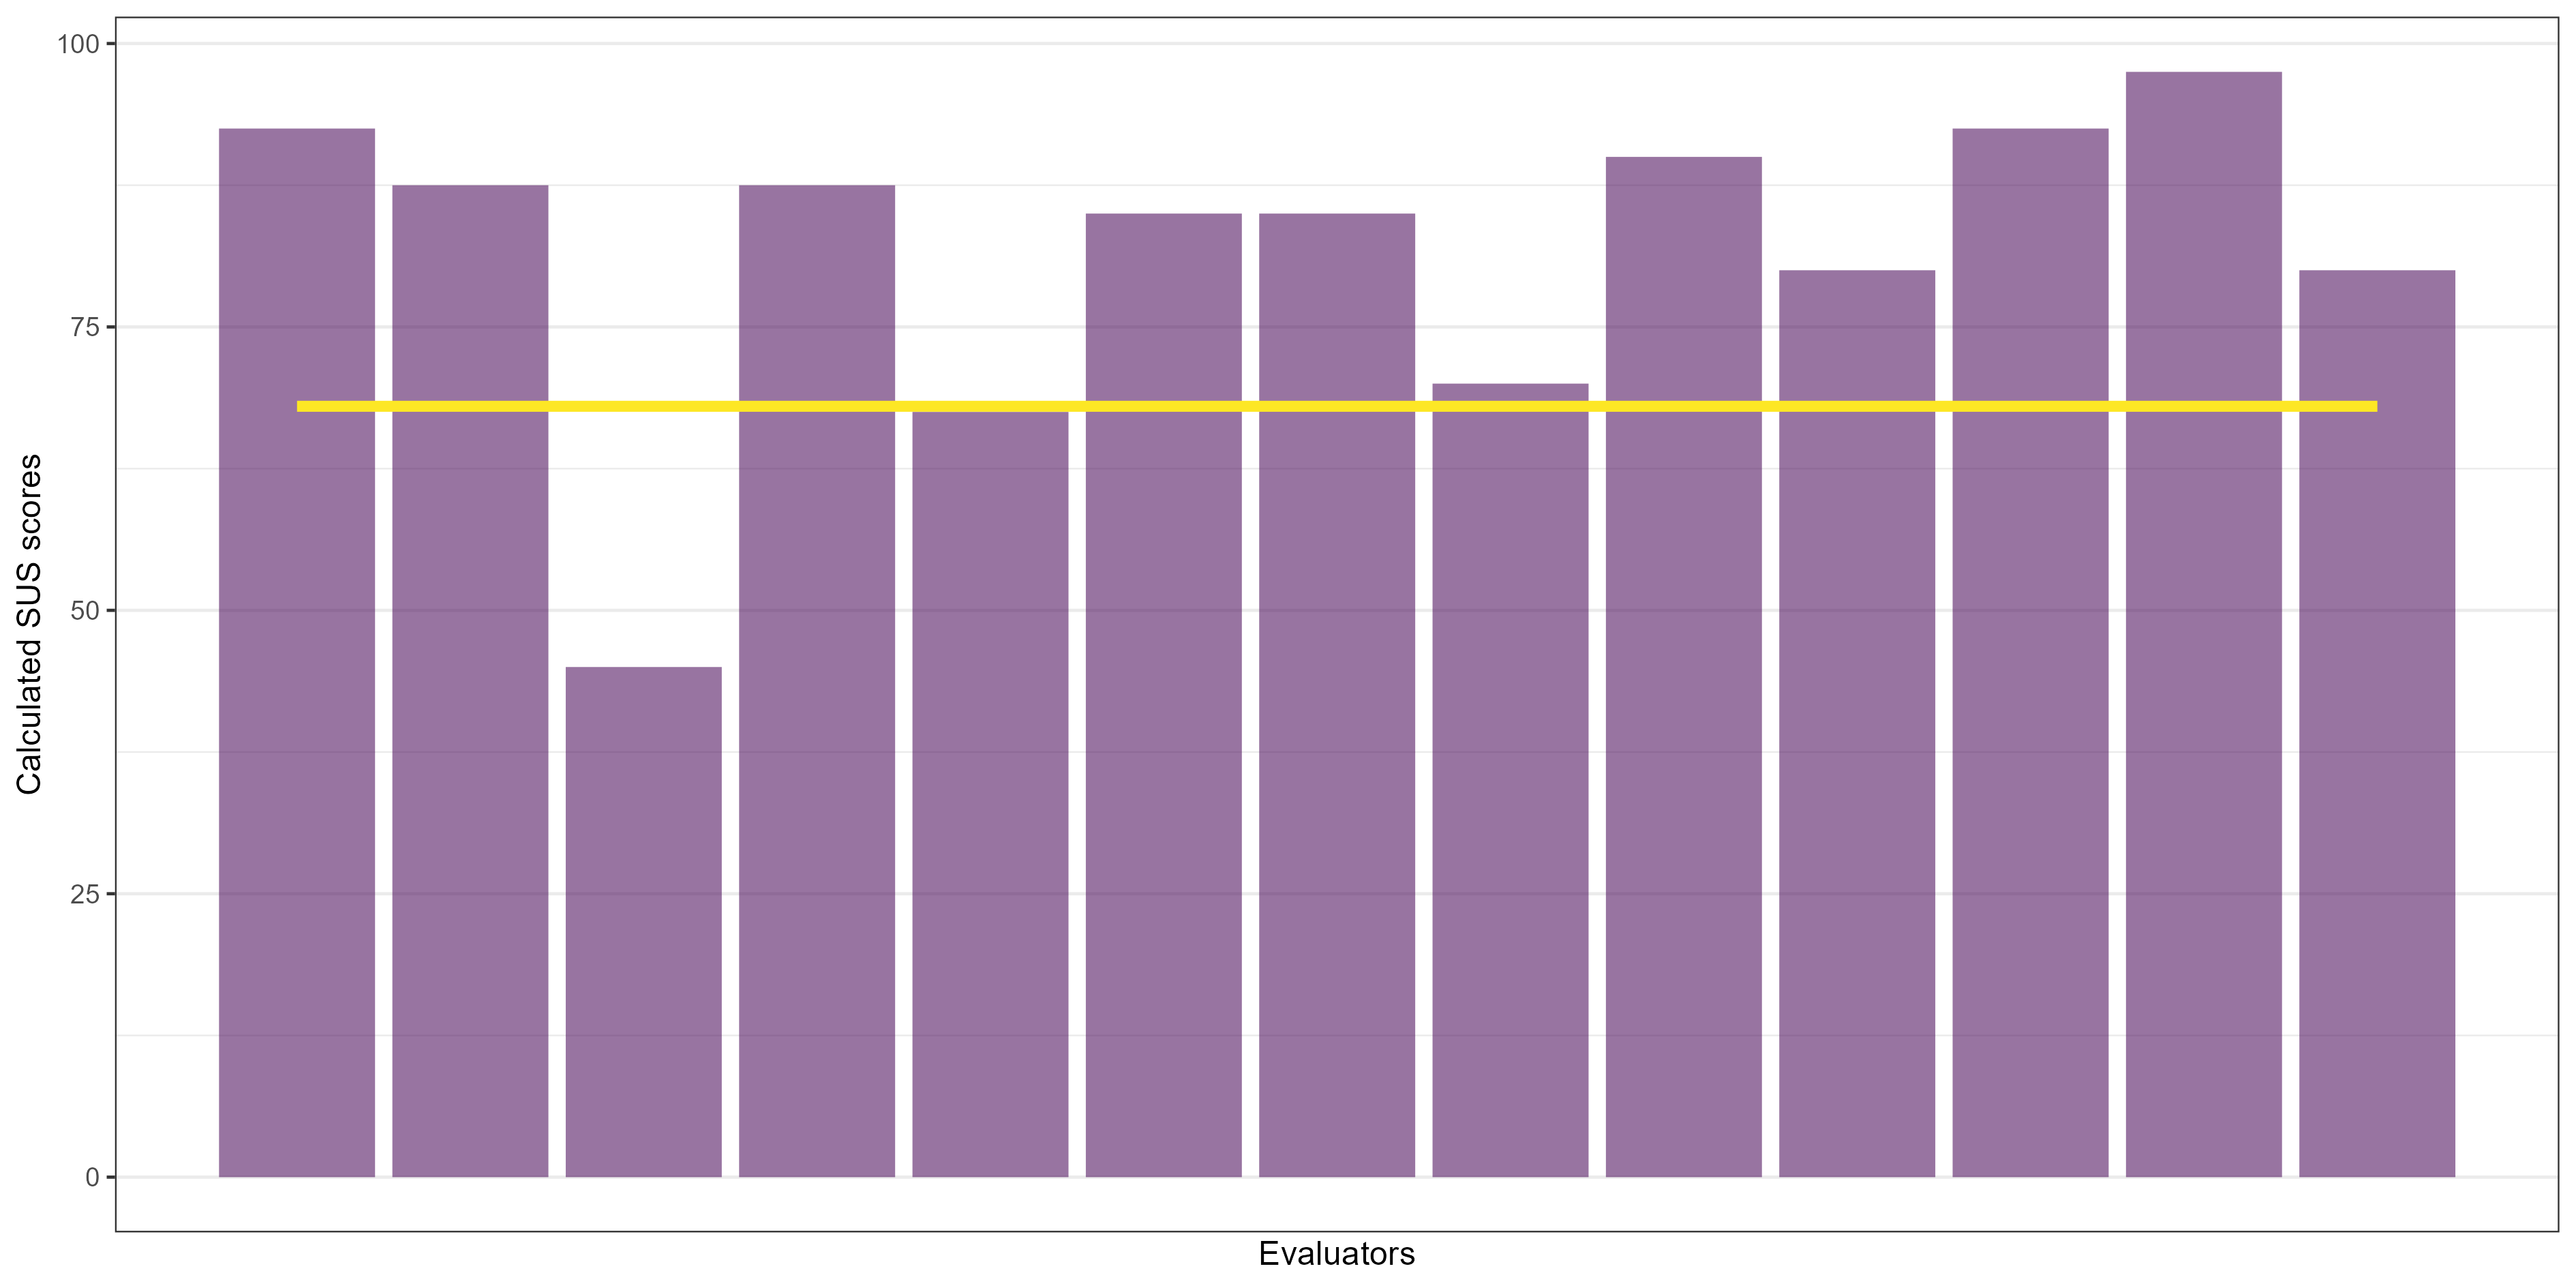
\includegraphics[width=1\linewidth]{images/sus_barchart.png}
    \caption{Bar chart of calculated SUS scores}
    \label{fig:sus_bar_visual} 
\end{figure}

\section{Responses to open-ended quetsions}
\label{appendix:user_eval_qual}

\subsection{Do you have any comments about the system after using it?}
\begin{itemize}
    \item Very easy use and a helpful first step towards a thematic analysis
    \item I think this is a really interesting project, and the quality of presentation of results is quite good. The one feedback I would give here is that when I tried to use the system before starting the questionnaire (the instructions on the landing page of the questionnaire linked to the system, so I just went there and tried to start using it), it was a bit difficult. I uploaded a large text file (oliver twist) and the system became unresponsive. Another smaller file became stuck too, maybe due to special characters. The FAQ addresses this, but I think the key instructions should be more prominent without having to go the FAQ. When I used it the way you are asked to in the questionnaire, it was a lot easier.
    \item I like it, sentiment analysis was very good and saves time, thematic analysis missed some things I noticed, but also caught some things I didn't on first reads - so could help stop researcher bias particularly in single researcher studies. Overall I would find it useful as a first stage of analysis to be expanded on and can see it saving me time.
    \item I think that the website could maybe have less pages but the system was really easy to use, maybe not that much interpret the results
    \item Very approachable and easy to use. Getting the results compiled in a PDF is a really great feature that I have not seen in any similar system previously.
    \item no
    \item The 90\_results folder I downloaded contained a pdf file that has a distorted table for the 3rd text (with a column width only a bit more than 4 cms)
    \item It was very user-friendly 
    \item Very professional
    
\end{itemize}

\newpage
\subsection{Do you have any suggestions on how to improve the system?}

\begin{itemize}
    \item No but enjoyed the opportunity to try it. Thanks
    \item This is pretty cool work as it is, maybe could be better from a general usability point of view (that is, imagine a person just coming to your home page without the instructions in the questionnaire, or the three files you share there). When the files are being processed, might be good to see some indication of this, and to see an error message if you load something that is not going to work. I enjoyed using this, thanks!
    \item As well as the existing help pages, integrating most of the help into the actual analysis process could be useful. For instance as part of a step by step form it instructs you how to prepare your documents, then upload them, etc. This might make it more useful for non technical / first time users - I spent some time switching between pages.
    \item Could be useful to integrate the About page and the Guides in the Home.
    \item It would be nice to be able to select which files to download instead of downloading a zip of all results.
    \item it's perfect as it is
    \item Nothing to improve
    \item Different website font

\end{itemize}







\end{appendices}

%==================================================================================================================================
%   BIBLIOGRAPHY   

% The bibliography style is abbrvnat
% The bibliography always appears last, after the appendices.

\bibliographystyle{abbrvnat}

\bibliography{l4proj}

\end{document}
